0%%%%%%%%%%%%%%%%%%%%%%%%%%%%%%%%%%%%%%%%%
% Masters/Doctoral Thesis 
% LaTeX Template
% Version 2.3 (25/3/16)
%
% This template has been downloaded from:
% http://www.LaTeXTemplates.com
%
% Version 2.x major modifications by:
% Vel (vel@latextemplates.com)
%
% This template is based on a template by:
% Steve Gunn (http://users.ecs.soton.ac.uk/srg/softwaretools/document/templates/)
% Sunil Patel (http://www.sunilpatel.co.uk/thesis-template/)
%
% Template license:
% CC BY-NC-SA 3.0 (http://creativecommons.org/licenses/by-nc-sa/3.0/)
%
%%%%%%%%%%%%%%%%%%%%%%%%%%%%%%%%%%%%%%%%%

%----------------------------------------------------------------------------------------
%	PACKAGES AND OTHER DOCUMENT CONFIGURATIONS
%----------------------------------------------------------------------------------------

\documentclass[
12pt, % The default document font size, options: 10pt, 11pt, 12pt
%oneside, % Two side (alternating margins) for binding by default, uncomment to switch to one side
%chapterinoneline,% Have the chapter title next to the number in one single line
english, % ngerman for German
onehalfspacing, % Single line spacing, alternatives: onehalfspacing or doublespacing
%draft, % Uncomment to enable draft mode (no pictures, no links, overfull hboxes indicated)
%nolistspacing, % If the document is onehalfspacing or doublespacing, uncomment this to set spacing in lists to single
%liststotoc, % Uncomment to add the list of figures/tables/etc to the table of contents
%toctotoc, % Uncomment to add the main table of contents to the table of contents
%parskip, % Uncomment to add space between paragraphs
%nohyperref, % Uncomment to not load the hyperref package
headsepline, % Uncomment to get a line under the header
]{MastersDoctoralThesis} % The class file specifying the document structure
\usepackage{amsmath, amsthm, verbatim,amssymb,graphicx, tikz, mathrsfs}%added by Yan Ju
\usepackage{bbm}%zheyang
\usepackage[utf8]{inputenc} % Required for inputting international characters
\usepackage[T1]{fontenc} % Output font encoding for international characters

\usepackage{palatino} % Use the Palatino font by default

\usepackage[backend=bibtex,style=authoryear,natbib=true]{biblatex} % Use the bibtex backend with the authoryear citation style (which resembles APA)

\addbibresource{ju.bib} % The filename of the bibliography

\usepackage[autostyle=true]{csquotes} % Required to generate language-dependent quotes in the bibliography

%----------------------------------------------------------------------------------------
%	MARGIN SETTINGS
%----------------------------------------------------------------------------------------

\geometry{
	paper=a4paper, % Change to letterpaper for US letter
	inner=2.5cm, % Inner margin
	outer=3.8cm, % Outer margin
	bindingoffset=2cm, % Binding offset
	top=1.5cm, % Top margin
	bottom=1.5cm, % Bottom margin
	%showframe,% show how the type block is set on the page
}

%----------------------------------------------------------------------------------------
%	THESIS INFORMATION
%----------------------------------------------------------------------------------------

\thesistitle{Essays on some mechanisms in the fields of auction, matching and mental competition} % Your thesis title, this is used in the title and abstract, print it elsewhere with \ttitle
\supervisor{Professor Guoqiang \textsc{Tian},   Zhe \textsc{Yang}} % Your supervisor's name, this is used in the title page, print it elsewhere with \supname
\examiner{} % Your examiner's name, this is not currently used anywhere in the template, print it elsewhere with \examname
\degree{PhD of Economics} % Your degree name, this is used in the title page and abstract, print it elsewhere with \degreename
\author{Yan \textsc{Ju}} % Your name, this is used in the title page and abstract, print it elsewhere with \authorname
\addresses{} % Your address, this is not currently used anywhere in the template, print it elsewhere with \addressname

\subject{Theoretical Economics} % Your subject area, this is not currently used anywhere in the template, print it elsewhere with \subjectname
\keywords{mechanism design, auction, matching, game theory} % Keywords for your thesis, this is not currently used anywhere in the template, print it elsewhere with \keywordnames
\university{\href{http://www.shufe.edu.cn}{Shanghai University of Finance and Economics}} % Your university's name and URL, this is used in the title page and abstract, print it elsewhere with \univname
\department{\href{http://econ.shufe.edu.cn}{School Of Economics}} % Your department's name and URL, this is used in the title page and abstract, print it elsewhere with \deptname
%\group{\href{http://researchgroup.university.com}{Research Group Name}} % Your research group's name and URL, this is used in the title page, print it elsewhere with \groupname
\faculty{\href{http://faculty.university.com}{Yan Ju}} % Your faculty's name and URL, this is used in the title page and abstract, print it elsewhere with \facname

\hypersetup{pdftitle=\ttitle} % Set the PDF's title to your title
\hypersetup{pdfauthor=\authorname} % Set the PDF's author to your name
\hypersetup{pdfkeywords=\keywordnames} % Set the PDF's keywords to your keywords

\begin{document}

\frontmatter % Use roman page numbering style (i, ii, iii, iv...) for the pre-content pages

\pagestyle{plain} % Default to the plain heading style until the thesis style is called for the body content

%----------------------------------------------------------------------------------------
%	TITLE PAGE
%----------------------------------------------------------------------------------------

\begin{titlepage}
\begin{center}

{\scshape\LARGE \univname\par}\vspace{1.5cm} % University name
\textsc{\Large Doctoral Thesis}\\[0.5cm] % Thesis type

\HRule \\[0.4cm] % Horizontal line
{\huge \bfseries \ttitle\par}\vspace{0.4cm} % Thesis title
\HRule \\[1.5cm] % Horizontal line
 
\begin{minipage}[t]{0.4\textwidth}
\begin{flushleft} \large
\emph{Author:}\\
%\href{http://www.johnsmith.com}
{\authorname} % Author name - remove the \href bracket to remove the link
\end{flushleft}
\end{minipage}
\begin{minipage}[t]{0.4\textwidth}
\begin{flushright} \large
\emph{Supervisor:} \\
%\href{http://www.jamessmith.com}
{\supname} % Supervisor name - remove the \href bracket to remove the link  
\end{flushright}
\end{minipage}\\[3cm]
 
\large \textit{A thesis submitted in fulfillment of the requirements\\ for the degree of \degreename}\\[0.3cm] % University requirement text
\textit{in the}\\[0.4cm]
\deptname\\[2cm] % Research group name and department name
 
{\large \today}\\[4cm] % Date
%\includegraphics{Logo} % University/department logo - uncomment to place it
 
\vfill
\end{center}
\end{titlepage}

%----------------------------------------------------------------------------------------
%	DECLARATION PAGE
%----------------------------------------------------------------------------------------

\begin{declaration}
\addchaptertocentry{\authorshipname}

\noindent I, \authorname, declare that this thesis titled, \enquote{\ttitle} and the work presented in it are my own. I confirm that:

\begin{itemize} 
\item This work was done wholly or mainly while in candidature for a research degree at this University.
\item Where any part of this thesis has previously been submitted for a degree or any other qualification at this University or any other institution, this has been clearly stated.
\item Where I have consulted the published work of others, this is always clearly attributed.
\item Where I have quoted from the work of others, the source is always given. With the exception of such quotations, this thesis is entirely my own work.
\item I have acknowledged all main sources of help.
\item Where the thesis is based on work done by myself jointly with others, I have made clear exactly what was done by others and what I have contributed myself.\\
\end{itemize}
 
\noindent Signed:\\
\rule[0.5em]{25em}{0.5pt} % This prints a line for the signature
 
\noindent Date:\\
\rule[0.5em]{25em}{0.5pt} % This prints a line to write the date
\end{declaration}

\cleardoublepage

%----------------------------------------------------------------------------------------
%	QUOTATION PAGE
%----------------------------------------------------------------------------------------

\vspace*{0.2\textheight}

\noindent\enquote{\itshape Thanks to my solid academic training, today I can write a whole doctoral thesis paper!}\bigbreak

\hfill Yan Ju

%----------------------------------------------------------------------------------------
%	ABSTRACT PAGE
%----------------------------------------------------------------------------------------

\begin{abstract}
\addchaptertocentry{\abstractname} % Add the abstract to the table of contents

Mechanisms Design is a very interesting field of economics. In this paper, theories about general mechanisms are presented as well as some kinds of special mechanisms such as matching. With all the needed 
details provided or given in the literature, the thesis is mostly a reflection of the author's interest and provide insightful arguments in related areas.

Under the interdependent value environment, the paper proposes a sufficient condition for ex post implementation of efficiency in an auction, i.e., allocating the good to the agent who values it most. This
condition is less demanding than a sufficient condition that is proposed in \parencite{Maskin00}. For the Chinese college admission mechanism, the paper finds that the allocation results of the ex post
equilibrium in the Boston Mechanism, Chinese parallel mechanism and the DA mechanism are the same. However, the ease for the DA mechanism to reach this allocation result can never be reached for the other two
mechanisms, which might be a motivation for advocating DA mechanism in the Chinese college admission mechanism. For a perfect information competitive board game like chess which is a mechanism
for deciding win or loss, the paper classify every position 
into three categories, winning position, losing position, and drawing position, and provides the way to identify them theoretically. Of course, it is only theoretical because the work need to be done is 
astronomical figure. 



\end{abstract}

%----------------------------------------------------------------------------------------
%	ACKNOWLEDGEMENTS
%----------------------------------------------------------------------------------------

\begin{acknowledgements}
\addchaptertocentry{\acknowledgementname} % Add the acknowledgements to the table of contents

Thanks to professor Guoqiang Tian for his teaching of Mechanism Design theory and advice to this doctoral paper, Zhe Yang for the cooperation we have been doing in publishing the paper 
``existence and generic stability of cooperative equilibria for multi-leader-multi-follower games'' which is primarily his idea. Thanks to all the teachers who has helped or taught me in SOE.

Thanks to all the classmates and friends that has been with me!

\end{acknowledgements}

%----------------------------------------------------------------------------------------
%	LIST OF CONTENTS/FIGURES/TABLES PAGES
%----------------------------------------------------------------------------------------

\tableofcontents % Prints the main table of contents

\listoffigures % Prints the list of figures

%\listoftables % Prints the list of tables

%----------------------------------------------------------------------------------------
%	ABBREVIATIONS
%----------------------------------------------------------------------------------------

\begin{abbreviations}{ll} % Include a list of abbreviations (a table of two columns)

\textbf{DA} & \textbf{D}eferred \textbf{A}cceptance \\
\textbf{SOSM} & \textbf{S}tudent \textbf{O}ptimal \textbf{S}table \textbf{M}atching\\
\textbf{TTC} &\textbf{T}op \textbf{T}rading \textbf {C}ycle\\
\textbf{SD} &\textbf{S}erial \textbf{D}ictatorship

\end{abbreviations}

%----------------------------------------------------------------------------------------
%	PHYSICAL CONSTANTS/OTHER DEFINITIONS
%----------------------------------------------------------------------------------------

%\begin{constants}{lr@{${}={}$}l} % The list of physical constants is a three column table

% The \SI{}{} command is provided by the siunitx package, see its documentation for instructions on how to use it

%	Speed of Light & $c_{0}$ & \SI{2.99792458e8}{\meter\per\second} (exact)\\
%Constant Name & $Symbol$ & $Constant Value$ with units\\

%\end{constants}

%----------------------------------------------------------------------------------------
%	SYMBOLS
%----------------------------------------------------------------------------------------

%\begin{symbols}{lll} % Include a list of Symbols (a three column table)

%$a$ & distance & \si{\meter} \\
%$P$ & power & \si{\watt} (\si{\joule\per\second}) \\
%Symbol & Name & Unit \\

%\addlinespace % Gap to separate the Roman symbols from the Greek

%$\omega$ & angular frequency & \si{\radian} \\

%\end{symbols}

%----------------------------------------------------------------------------------------
%	DEDICATION
%----------------------------------------------------------------------------------------

\dedicatory{Dedicated To my parents who has been so patient and loving to me since my birth} 

%----------------------------------------------------------------------------------------
%	THESIS CONTENT - CHAPTERS
%----------------------------------------------------------------------------------------

\mainmatter % Begin numeric (1,2,3...) page numbering

\pagestyle{thesis} % Return the page headers back to the "thesis" style

% Include the chapters of the thesis as separate files from the Chapters folder
% Uncomment the lines as you write the chapters


% Chapter 1

\chapter{An Introduction to Mechanism Design Theory} % Main chapter title

\label{Chapter1} % For referencing the chapter elsewhere, use \ref{Chapter1} 

%----------------------------------------------------------------------------------------

% Define some commands to keep the formatting separated from the content 
\newcommand{\keyword}[1]{\textbf{#1}}
\newcommand{\tabhead}[1]{\textbf{#1}}
\newcommand{\code}[1]{\texttt{#1}}
\newcommand{\file}[1]{\texttt{\bfseries#1}}
\newcommand{\option}[1]{\texttt{\itshape#1}}

\newtheorem{definition}{Definition}
\newtheorem*{definition*}{Definition}
\newtheorem{thm}{Theorem}
\newtheorem*{thm*}{Theorem}
\newtheorem{example}{Example}
\newtheorem*{example*}{Example}
\newtheorem{lemma}{Lemma}
\newtheorem*{lemma*}{Lemma}
\newtheorem{prop}{Proposition}
\newtheorem*{prop*}{Proposition}
\newtheorem{assumption}{Assumption}
\newtheorem*{assumption*}{Assumption}
\newtheorem{corollary}{Corollary}
\newtheorem*{corollary*}{Corollary}
\newtheorem{conjecture}{conjecture}
\newtheorem*{conjecture*}{conjecture}
\newtheorem*{remark}{Remark}



%----------------------------------------------------------------------------------------


 
%------------------------------------------------------------------------------------------




%----------------------------------------------------------------------------------------

\section{Introduction}

The starting point of analysis in traditional economics is often the
present state of economic institutions and mechanisms, for example,
market theory, auctions and resource allocation. In mechanism design
theory, an alternative framework and perspective is used. We view the
present state of affairs just as a possibility and has an intention to
design a better mechanism with respect to a social goal or
criterion. Mechanism design is kind of engineering side of
economics. To do that, a framework must be provided. Now the framework
has become a theory with a large body of literatures. That theory is
mechanism design theory. The mechanism design theory was established
by leonid Hurwicz, later expanded by Roger B.Myerson, Eric S. Maskin,
Guoqiang Tian and many other  scholars of the field.

 The most important
component of Mechanism design theory is implementation
theory. \parencite{Liang2010} has done a survey of this field
.  The present paper is not another attempt to summarize the
implementation theory of mechanism design, but uses it as  a central tool for formalizing ideas
in this paper. This paper aims  to analyze some
economic mechanisms for situations where information  is not
fully known to the social planner. In the process, the author creates some new
concepts which the author thought is necessary. However, a little
background of the mechanism design theory is needed. This is what the next
section is about.

\section{A survey of the background}

A formal study of the informational requirements and informational optimality of resource
allocation processes was initiated by Hurwicz (1960).  In line with the prevailing tradition, interest in this area was focused
on the design of Pareto-satisfactory (non-wasteful) and privacy-preserving mechanisms, i.e.,
mechanisms that result in Pareto efficient allocations and use informationally decentralized
decision making processes.  Allocative efficiency and informational efficiency are two highly
desired properties for an economic system to have.  The importance of Pareto optimality is
attributed to what may be regarded as a minimal welfare property. Pareto optimality requires
resources be allocated efficiently. If an allocation is not efficient, there is a waste in allocating
resources and thus at least one agent is better off without making others worse off under given
resources. Informational efficiency requires an economic system have the minimal informational
cost of operation. The informational requirements depend upon two basic components: the class
and types of economic environments over which a mechanism is supposed to operate and the
particular outcomes that a mechanism is required to realize.

For informational decentralized systems, \parencite{Hurwicz1972}
proved a very important theorem: For the neoclassical pri-
vate goods economies, there is no mechanism < M, h > that implements Pareto efficient
and individually rational allocations in dominant strategy. Consequently, any revelation
mechanism < M, h > that yields Pareto efficient and individually rational allocations is
not strongly individually incentive compatible. (Truth-telling about their preferences is not
Nash Equilibrium).

A mechanism can be viewed as an abstract planning procedure; it consists of a message
space in which communication takes place, rules by which the agents form messages, and an
outcome function which translates messages into outcomes (allocations of resources). Mecha-
nisms are imagined to operate iteratively. Attention, however, may be focused on mechanisms
that have stationary or equilibrium messages for each possible economic environment. A mecha-
nism realizes a prespecified welfare criterion (also called performance, social choice rule, or social
choice correspondence) if the outcomes given by the outcome function agree with the welfare
criterion of the stationary messages. 

\section{General model framework}
 In this section, we give the framework of analysis which will
 reappear many times later in the paper with slightly different
 forms. Our framework is comprised of 5 parts: 
 economic environments, social goals or criteria,  mechanism, 
expected outcomes(often equilbirums of all kinds), and the concept of
implementation of social goals.
The following subsections will give a detailed discussion and relative
notations of these components.
\subsection{Economic environments}
Economic environments consists of economic entities and their features
as well as the state of some relevant things in the world. The
entities are of two kinds. One is the principal (or called the social
planner),  and the other is  the agents (or called economic
participants).  Usually, we have the following notations.

$N=\{1,...,n\}$: denote the set of the agents.

$e_i\in E_i$: denote the economic feature of agent $i\in N$. It may be preferences, economic status or some other relevant feature.

$E=E_1\times \dots \times E_2$: denote the set of profiles of economic features.

 The social planner does not know much information of
the participants' profile $e$. These information are decentralized
among the agents. 
If the agents all know the whole profile $e$, then it is the perfect information case; if every agent $i$ knows his own $e_i$ and knows the distribution of $e$, then this is the imperfect information case which can be dealt with using Bayesian method; else if every agent $i$ only knows his own $e_i$, then it is only good to be dealt with using strategyproof mechanisms. The details will be in later chapters.

\subsection{Social criteria}

Given an economic environment $e$, every agents participate in economic activities, make economic decisions, pay the cost and get the profits. The social planner hope that the results satisfy some criteria.
Let us give some notations and talk about it.

$A$: denote the set of social allocations, or economic results.

$F : E \mapsto A$: denote a social criterion, or social goal, which is a correpondence from the set of environments to the set of results. Given any environment $e$, there will be a subset of $A$ that satisfy the social criterion, $F$ just denotes this function.

If randomized results on $A$ are acceptable as social results, then we can use 
$\Delta A$ instead of just $A$. 

\subsection{Mechanism for information collection}

 The social planner lacks information, so he or she need to design incentive
compatible rules of the game to induce everyone reveal their true private information. 

If the social planner knows completely the environment, then he or she
can simply choose a result that is in the set $F(A)$. However, he or
she usually does not know much about these things. That is where
mechanism for information collection functions.  A mechanism, or  a
game form, usually contains the following components.

$M_i$: denote the message space of agent $i \in N$. An agent can only emit 
message $m_i \in M_i$.

$M=M_1\times\dots\times M_n$: denote the space of message profiles. Every message profile $m=(m_1,\dots,m_n)\in M$.

$h:M\rightarrow A$: denote the assignment function for the mechanism, which assigns a result for a given message profile $m$.

$ \Gamma = \langle M,h\rangle$: denote the information collection mechanism, which is just the combination of the space of message profiles and the assignment function that lies on top of it.

Thus, a mechanism prescribes rule of the game. Every agent $i$ chooses a message
$m_i \in M_i$ to send, and then the social planner collects all the messages in the message profile $m$, and finally decides on the allocation result $h(m)$ as the social choice. The $\Gamma$ must be declared openly to let every agent know, then it is up to every agent $i$ to choose from his or her $M_i$ the $m_i$ to report.

A very important class of mechanisms is the direct revelation
mechanism(or simply called direct mechanism) in which $M_i$ is just the possible world state information 
that agent $i$ has.  later we will introduce a very important theorem
about this mechanism.
\subsection{Expected outcomes}

When a mechanism $\Gamma=\langle M, h\rangle$ is given, we have a game
with rules for the agents to report $m \in M$. The strategy of an
agent $i$ is usually denoted $\sigma^i(e_i,\Gamma)$ or $\rho^i(e_i,\Gamma)$. Taking this
form is for the reason that different environments $e_i$ may induce
$i$ to choose different message for a given mechanism $\Gamma$. For a given $\Gamma$, the $\Gamma$ in the above notation can usually
be omitted as the default $\Gamma$ is clear.
When the agents send messages to the social planner, they have strategical interaction in choosing which message to send. Now we need to know what will result from the strategical interaction, these are the expected outcomes. Usually the solution concept of equilibriums in games are ideal for this role.

Here, one point concerning the $e$ should be stressed.  There is requirement on the preference
information which is contained in $e_i$ for every $i \in N$.
When people game with each other, the hypothesis for human behavior is
very important. A fundamental hypothesis is that human being are
self-interested, that is, they will try to maximize some kind of
self-utility. With this hypothesis, it is usually implied that human
being will not deliberately contribute to the society without
considering the returns to himself or herself. Or put it another way,
a human being will only concentrate on maximizing self-interest, only
a good mechanism can make this self-interesting behavior also
beneficial to the society. Let $\succeq_{e_i}$ denote the preference
in $e_i$ for agent $i$. It must be an order relation on the results
set $A$. Put it another way, it must satisfy the following 3
conditions.

\begin{itemize}
\item Reflexivity. For any outcome $a \in A$, $a\succeq a$.
\item Completeness. For any two outcomes $a$ and $b$ from $A$, either $a\succeq
  b$ or $b\succeq a$. That is , any two outcomes are comparable.
\item Transitivity. For any three outcomes $a$, $b$ and $c$, if both
  $a \succeq b$ and $b \succeq c$ hold, then $a \succeq c$ hold. This
  eliminates unwanted circles.
\end{itemize}

Two other relations $\succ$ and $\sim$ can be generated from a given
$\succeq$.
For any $a$ and $b$ from the results set $A$, $a \succ b$ if and only
if $a \succeq b$ and $b \not \succeq a$; $a \sim b$ if and only if  $a
\succeq b$ and $b \succeq a$. 

The three relations $\succeq, \succ,\sim$ are also frequently denoted
with a single letter $R, P, I$ respectively. Later, we will use these
single letter forms for consistency with matching literature in that
chapter.


With this kind of preference, every agent $i$ can rank the results in
$A$ in such a way that equilibriums are definable.

With this hypothesis, the equilibrium concepts of game theory best suit our needs for the expected outcomes. The equilibriums are the expected outcomes. For different situations, different equilibrium concepts should be taken as the expected outcomes. Dominant strategy equilibrium, Nash equilibrium, Subgame perfect Nash equilibrium, Bayesian Nash equilibrium, Perfect Bayesian equilibrium and so on all have their chances of being the expected outcomes depending on the problem situation. Notations are as follows.

$b(e,\Gamma)$: denote the equilibrium message choices $M* \subset M$ under the economic environment $e$ and mechanism $\Gamma$.

$h(b(e,\Gamma))$: denote the expected outcomes of the assignment.

For a given $\Gamma$, the $\Gamma$ in the above notation can usually
be omitted as the default $\Gamma$ is clear.






  

\subsection{Implementation of social criteria}

Finally, comes the concept of implementation. An important goal of
mechanism design is to make individual incentives and social criteria
compatible.  Roughly speaking, if a social criteria is satisfiable under certain
equilibrium solution of a mechanism, then we say that that social
criteria is implementable with that mechanism.
The idea can be illustrated by the following graph.

\begin{center}
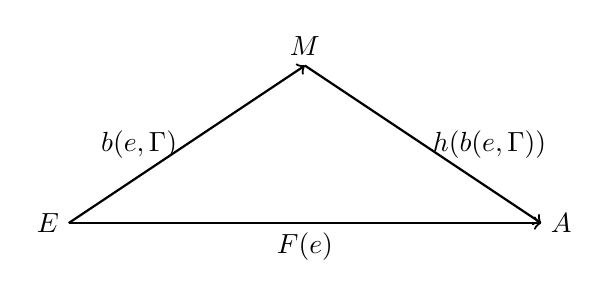
\begin{tikzpicture}
\draw [->] [thick] (1,0) --  (7,0);
\node [below] at (4,0) {$F(e)$};
\draw [->] [thick] (1,0)--(4,2);
\node [left] at (2.5,1) {$b(e, \Gamma)$};
\draw [->][thick] (4,2)--(7,0);
\node [right] at (5.5,1) {$h(b(e,\Gamma))$};

\node [above] at (4,2) {$M$};
\node [left] at (1,0) {$E$};
\node [right] at (7,0) {$A$};

\end{tikzpicture}

\end{center}

In the above graph, $e \in E$ is the economic environment, $A$ is the
possible allocation set. Social criteria $F$ choose what is desirable
allocation for the society. The social planner need to design a
mechanism to implement the criteria. Under such a mechanism,  the
strategic interaction of agents should result in an outcome in the
equilibrium set $b(e, \Gamma)$ mapped by $h$, i.e.,
$h(b(e,\Gamma))$. If $h(b(e,\Gamma))$ is in the set $F(e)$,  then the
social criteria have been implemented. Formally, we have the following
definition

\begin{definition}
A mechanism $\Gamma=\langle M,h\rangle$ is said to have implemented the social
criteria $F$ in the economic environments space $E$ under the
equilibrium $b$, if for all $e \in E$, we have $h(b(e,\Gamma)) \subset F(e)$.
\end{definition}

Our implementation concept in this paper is weak compared to most in
the literature.  And what we call social criteria $F$ is usually
called social choice, by choosing the wording ``criteria''  we want to convey the idea that not
every  point  in $F(e)$ must be implemented.  However, we still
distinguish between two forms of weak implementation. 

Here is the weaker implementation concept definition that we call
partial 
implementation.

 \begin{definition}
A mechanism $\Gamma=\langle M,h\rangle$ is said to have partially implemented the social
criteria  $F$ in the economic environments space $E$ under the
equilibrium $b$, if for all $e \in E$, we have $h(b(e,\Gamma)) \cap
F(e) \not = \emptyset$.
\end{definition}


Below is the strongest implementation concept that we call full
implementation.

 \begin{definition}
A mechanism $\Gamma=\langle M,h\rangle$ is said to have fully implemented the social
choice rule  $F$ in the economic environments space $E$ under the
equilibrium $b$, if for all $e \in E$, we have $h(b(e,\Gamma)) = F(e)$.
\end{definition}



The above five-component framework covers both the literature review of chapter 2 as well as the messaging
mechanisms of auction and matching we will later discussed in-depth in
Chapter3 and Chapter4.

For these kind of mesaging mechanism, there is a very famous
theorem called revelation principle. I will give here its definition
and the proof is given in Appendix \ref{Appendix_A}.

\begin{thm*}
revelation principle:

if a Mechanism $\langle M, h\rangle$ implements the social criteria 
$F$ in dominant strategy
equilibrium. Then there is a direct revelation mechanism which
implements $F$ truthfully in dominant strategy equilibrium(truth
telling is a dominant strategy equilibrium). 

\end{thm*}

The importance of revelation principle lies in the fact that it narrowes the search space for an implementation mechanism to a special kind of mechanism. This makes the finding of a mechanism implementing some social goal more easily or give a method of proving the nonexistence of such mechanism in general by just proving the unavailability of such mechanism for the revelation games.

\section{Some examples of  mechanisms}

The previous introduction of general model is abstract. The following subsections will give two examples of mechanism design in more concrete situations. These exemplifies the usefulness of mechanism design. They can be safely skipped without hindering reading of later chapters.

\subsection{Assets Inheritance problem}
\label{assets_inheritance}
\begin{example}
An old man has lots of  houses and three sons. When he is about to die, he
want to give the houses to his sons, but he is not familiar with the
market prices for these houses. He does not want to make the sons
share any house, so he would like to  give every  house as a whole to some son. All  sons know the prices of these
houses well. all  sons like more values from the
inherited houses. How can he achieve his goal of dividing the houses as
fairly\footnote{The fairness here means that to make the least valued group of assets as valuable as possible.} as possible, and if it can not be perfect fair, he prefers to
give his younger sons more. 



\end{example} 

For the example situation, can a mechanism be designed so that the old
man's goal be implemented? The best mechanism should be let the oldest son to devide the assets or houses into 3 groups, then let the youngest son chooses first, and the middle son chooses second, and the oldest
son gets what is left. This is the simple but effective way of implementing the choice rule.

Another implementing  mechanism that constitutes a revelation game is that let the three sons report the values of the assets
. and then devide the assets as fairly as possible according to what the oldest son has reported(he divides the houses to let the least valued group of houses as valuable as possible). The social planner picks the most valuable group of assets according to the youngest son's report and 
give it to him, 
then picks the more valuable group from the remaining assets according to the middle son's value report, and finally gives the last group of goods to  the oldest son. 

\begin{comment}
In fact, the existence of the second mechanism is implied by the existence of the first mechanism by a simple application of revelation principle.If due to some reason for implementation, a revelation mechanism is more preferred, whenever we have chanced upon a mechanism implementing some social goal, we can convert it to a revelation mechanism which is called the equivalent direct mechanism of the original mechanism. You can see Chapter \ref{Chapter4} for a conversion of some Chinese college admission mechanisms into equivalent direct mechanism forms.
\end{comment}


\subsection{An example of Auction Design}
In the last part of the chapter, we would like to design a mechanism for selling goods with  uncertain values.  Here a distribution assumption is used. Auctions are one of the most successful areas where the development of economics
theory and practice help each other. I will try to investigate this area from
a mechanism design perspective in this section. The material is put here as an example of what can be implemented for some special market. 

Here we focus on revenue maximization for the seller of an indivisible experience
good under a situation in which buyers are all ex-ante identical. The only information they all have is an identical
value distribution of the experience good. In our
setting, the seller can freely give any buyer access to get his true private value, which process we call experiencing the good. If the seller is
unable to charge experience fee, she may maximize her revenue by excluding just one buyer from experiencing, which is in conflict with the social efficiency. If
the seller is able to charge experience fee, she will maximize her revenue through setting
the price at a level such that every potential buyer will buy the experience, 
resulting in the maximal trading surplus which is fully extracted by the seller.

Of course, the equilibrium of implementation in such a mechanism is ex ante,  the following chapter will be concerned with ex post implementation.

Now the details are as follows. A seller(she) has a single indivisible good, and wants to sell the good to a group of $N$ buyers indexed by $i=1, 2, . . . , N$(buyers and
bidders are used interchangeably in this paper, and are assumed to be
male). All parties are risk neutral. 
 The value of retaining the good to the seller
is publicly known as $\underline{v}(\geq 0)$ in this paper. Bidder i's valuation of the object
is $v_{i}$, and $v_{i}$ has independent identical distribution $F(x)$ with support $[\underline{v}, \overline{v}]$, 
where $\overline{v}>\underline{v}$, and $\overline{v}=+\infty$ is allowed. 
In the beginning, no one can directly observe the $v_{i}$. Only the distribution is common knowledge among all the parties. However, if the seller gives a chance of experiencing the good to a buyer, the buyer can learn of his $v_{i}$ after experiencing. 
 

The seller designs a sales mechanism to sell the
good. The sales mechanism consists of two stages, the experience stage, and the auction stage. 
After the experience stage, the seller will allow those who
have experienced the good to
participate the auction. By Revenue Equivalence Principle, we analyze the case that the seller chooses the second-price
sealed-bid auction in the auction stage without loss of generality. In the auction stage, if no bidder bids a value exceeding a reserve price
, then the good is sold to the unexperienced buyer at the
price $\mu$(the expectation of v) when there is an unexperienced buyer. Here we assume that the buyer will choose to buy the good if he is indifferent between buying and not buying the good. 
The timeline is shown in the Figure 1. 
\begin{figure}
\begin{center}
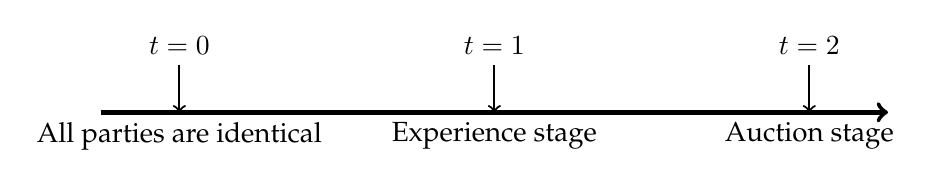
\begin{tikzpicture}
 \draw[->, ultra thick] (5, 0) -- (15, 0);
 \draw[->, thick](6, 0. 6)node[above]{$t = 0$} -> (6, 0)node[below]{All parties are identical } ;
 \draw[->, thick](10, 0. 6)node[above]{$t = 1$} -> (10, 0)node[below]{Experience stage};
 \draw[->, thick](14, 0. 6)node[above]{$t = 2$} -> (14, 0)node[below]{Auction stage} ;
 \end{tikzpicture}
\end{center}
 \caption{Timing of experience good auction }
\end{figure}

\subsubsection{Setting Reserve price to extract trade surplus}
In the situation that the seller cannot charge fee for experiencing the good, 
the seller will set a reserve price in the auction stage to maximize the
revenue in a second-price sealed-bid auction. 
\begin{lemma}\label{lem}
 The hazard rate function associated with the distribution F is
defined as $\lambda(x) = f(x) / (1 - F(x))$. The optimal reserve price $r$ satisfies $r - 1/\lambda(r)= v^*$. The $v^*$ denotes the seller's reserve revenue/valuation. 
\end{lemma}
\begin{proof}
Let $R(r, m)$ denote the revenue of the seller when the reserve price is $r$ and the number of buyers experiencing the good is $m$. 

Obviously, $r$ should be higher than $v^*$ to have an effect of enhancing the price. 
Then the expected value of seller revenue can be calculated as the sum of three parts, the revenue from the auction when the second highest bid is above the reserve price $r$, the revenue from the auction when the highest bid is above the reserve price but the second highest price is below the reserve price $r$, and the reserve revenue/valuation$v^*$ when the highest bid is below the reserve price $r$. 
\begin{equation}\label{equ}
R(r , m) =\int_{r}^{\overline{v}}x\mathrm{d}G_{(2)}^{m}(x) + rmF^{m-1}(r)[1 - F(r)] + v^* F^{m}(r)
\end{equation}
where $G_{(2)}^{m}(x) = F^{m}(x) + mF^{m-1}(x)[1 - F(x)]$. 


Differentiating this with respect to $r$ and simplify, we obtain
$$-rmF^{m-1}f(r)+mF^{m-1}(r)(1-F(r))+v^* mF^{m-1}(r)f(r)$$

The first order condition is 
$$r^* - \frac{1 - F(r^*)}{f(r^*)} = v^*$$
\end{proof}
\begin{remark}
 Under regularity conditions, the first order condition is also sufficient for optimality. 
\end{remark}
 If the seller gives a buyer the chance to experience the good, no buyer will refuse since experiencing the good means some chance
of gain. Thus the number of buyers who can experience the good is at her control. Intuitively, she 
wants to obtain a high revenue from the auction by letting more buyers to experience as long as there is still an unexperienced buyer, for the seller can sell the good to him
at price $\mu$ when no bidder bids over the
reserve price. This is summarized in the following proposition. 
\begin{prop}
 As the number m of buyers experiencing the good increases, the expected value of seller revenue increases as long as $m\leq n-1$. 
\end{prop}
\begin{proof}
When the reserve revenue $v^*$ is obtained by selling the good to a 
unexperienced buyer, $v^*=\mu$. Then by equation~\ref{equ} in the proof of Lemma~\ref{lem}, 
\begin{equation}
R(r, m) = \int_{r}^{\overline{v}}x\mathrm{d}G_{(2)}^{m}(x) +
rF^{m-1}(r)[1 - F(r)] + \mu F^{m}(r)
\end{equation}
where $G_{(2)}^{m}(x) = F^{m}(x) + mF^{m-1}(x)[1 - F(x)]$. 

When $m\leq N-1$, the best reserve price is $r=r^*$ which is the solution to $r^*-1/\lambda(r^*)=\mu$. The revenue is $R(r^*, m)$. 
 By the first order stochastic dominance, it is straightforward to show $R(r^*, m) > R(r^*, m')$ for any $N-1\geq m>m'$. 
\end{proof}
However, letting $N$ potential buyers to all experience the good may
not be better than just letting $N-1$ buyers to experience. Because the former may let go the
safe option of selling the good at $\mu$. Indeed, it depends on the
distribution F(x). A careful research of us has led to the following conclusion. 
\begin{thm}
 The seller does not always want all buyers to experience the good under the setting here. 
 \end{thm}
 \begin{proof}
 When every buyer has experienced the good, then by lemma~\ref{lem}, 
 the reserve price should now be set to $\hat{r}$, which is the solution to $\hat{r}-1/\lambda(\hat{r})=\underline{v}$, since the reserve
valuation is $\underline{v}$ and the revenue 
is $R(\hat{r}, N)$ using equation~\ref{equ}. 
Generally speaking, 
 $R(\hat{r}, N)<R(r^*, N-1)$ for many distributions and the potential buyers' number N. 
 \end{proof}
Figure 2 shows the values of $R(r^*, N-1)-R(\hat{r}, N)$ for different
values of parameters in Beta distribution(with the horizontal axis denoting N). 
\begin{figure}
\centering
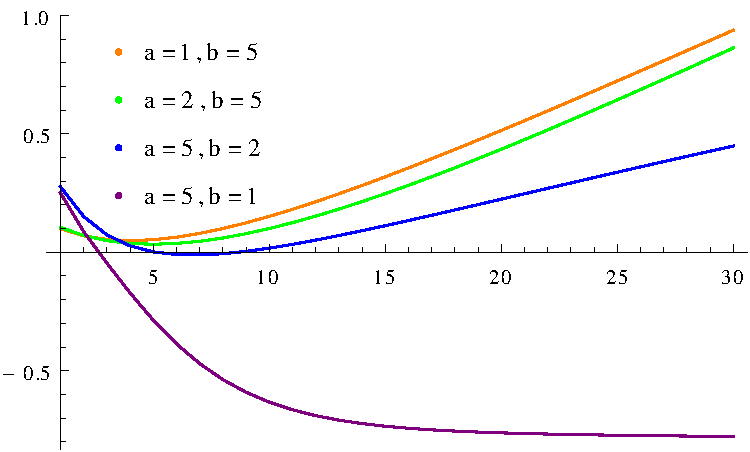
\includegraphics[width = 11cm]{betaGraph.pdf}
\caption{Difference in revenue: $R(r^*, N-1)-R(\hat{r}, N)$} \label{fig:graph}
\end{figure}

\begin{remark}
 Specially for the uniform distribution, we have, when $N\leq 7$, $R(\hat{r}, N)<R(r^*, N-1)$. 
\end{remark}

\subsubsection{Charging Experience fee to extract trade surplus}
 We then consider the case where the seller can charge experience fee. For the seller, at the experience-stage, how to optimally set price of exprience? 
If a certain number of buyers are permitted to experience the good, each of those buyers is supposed to get a nonnegative ex ante expected payoff from participating the
subsequent second-price auction. Suppose that buyers will buy the experience when they are indifferent between remaining
uninformed and buying the experience to be informed. 
 Then the seller should set the price equal to a buyer's ex ante expected payoff of participating the auction to extract all the expected trade surplus. Intuitively, the ex ante expected payoff of experiencing buyers depends on the number of auction partipants. 
%First, we set the prespecified price as $\mu$ for the auction. Then the expected result of the auction can be calculated. \end{comment}



Next, we will offer the formula for the experience fee in the following lemma. 
\begin{lemma}
 The experience fee $P(m)$ can be formulated as 
\begin{equation}
 P(m) = \begin{cases}\int_{\mu}^{\overline{v}}\int_{\mu}^vF^{m-1}(t)\mathrm{d}tf(v) \mathrm{d} v, &\textrm{if}\quad m \leq N-1\\
\int_{\underline{v}}^{\overline{v}}\int_{\underline{v}}^v F^{N-1}(t)\mathrm{d}tf(v) \mathrm{d} v, &\textrm{if}\quad m = N
\end{cases}
\end{equation}


\end{lemma}
\begin{proof}
 When there are $m(\leq n-1)$ buyers knowing one's own value information, the value of the information is
\begin{align*}
P(m)&= \int_{\mu}^{\overline{v}}(\int_{\mu}^v (v-t)\mathrm{d}F^{m-1}(t)+(v-\mu)F^{m-1}(\mu))f(v)\mathrm{d}v \\
&= \int_{\mu}^{\overline{v}}\int_{\mu}^vF^{m-1}(t)\mathrm{d}tf(v)\mathrm{d}v
\end{align*}

$P(N)$ can be formulated as, 
 \begin{align*}
P(N) &= \int_{\underline{v}}^{\overline{v}}\int_{\underline{v}}^v(v-t)\mathrm{d}F^{N-1}(t)\mathrm{d}tf(v)\mathrm{d}v \\
 &= \int_{\underline{v}}^{\overline{v}}\int_{\underline{v}}^v F^{N-1}(t)\mathrm{d}tf(v)\mathrm{d}v
\end{align*}
\end{proof}

\begin{lemma}
As the number of buyers knowing one's own value information increases, the expected value of knowing one's own value information decreases. 
\end{lemma}
Notice that for many distributions and potential buyers' number n, $P(N) < P(N-1)$. In such cases, the seller set price at $P(N)$, and 
the buyers' domininant stratey is to buy the experience. 
Since every buyer knows the true value in the auction and expected gain of every buyer is zero now, the seller can extract full surplus through setting appropriate experience fee. the 
social surplus is maximized and fully extracted by the seller. 



The above reasoning leads to the following conclusion

\begin{thm}

 If the seller can charge fee for letting one buyer know his true value, then the seller will set the price
 $ \int_{\underline{v}}^{\overline{v}}\int_{\underline{v}}^v F^{n-1}(t)\mathrm{d}tf(v)\mathrm{d}v$ to fully extract all the surplus of trade, and the revenue she get is 
 \begin{equation}
 E(V_{(1)}^N)=\int_{\underline{v}}^{\overline{v}} x\mathrm{d}F^N(x) 
 \end{equation}
where $V_{(1)}^N$ denotes the highest bid. 
\end{thm}
 This is the best possible result for the seller, maximizing the trade surplus and minimizing all the buyers' share. 


The example is supposed to shed light on a seller's optimal
sales mechamism design when buyers have identical value distribution about the
experience good, but do not know the private value before the experience. The seller controls the number of buyers to experience. 

When the seller is not able to charge experience fee, her optimal sales mechanism might be to exclude a buyer from experiencing the good, which harms social
 efficiency. When the seller is allowed to charge fee, the result is efficient. However, the defect is that
 all the trade surplus is extracted by the seller. 




 

 

\section{Mechanisms we will discuss}

In this section, I would like to talk about the scope of my
thesis. The main focus will be around mechanisms for dealing with
decentralized information problem. The last chapter is a diversion to
some
mechanisms that are designed for special purpose and under special requirements.4 chapters follow this introductory one.

 Chapter 2 is a review of important results in the literatures of mechanism design and Nash implementation, especially those
impossibility results. These results establish the impossibility of implementability with most general conditions. And this lead us to put effort in the consideration of more specific environments and conditions. The body of theory on Perfect Information Nash implementation exemplify the method mostly employed in the search. They proposed conditions and then through method of construction proved that under the conditions certain social goal can be Nash implemented.

Chapter 3 is a whole chapter devoted to the study of ex post implementation of socially efficient allocation goal through money transfer under the interdependent value environment. The material in this chapter employ the condition-proposing and constructive-proving method frequently found in mechanism design literature. Both continuous and discrete cases are considered. A sufficient condition called Condtion $\rho$ for ex post implementation with interdependent values via money transfer is given for the multiple goods assignment problem as an attempt to contribute to the field. 

Chapter 4 is devoted to a discussion of matching mechanisms design. The attention is later focused on an application of the theory to the Chinese college admission mechanism. A few derived propositions show that the score-dictating mechanism is perhaps the best choice among three popular mechanisms.

Chapter 5 is a chapter reflecting upon a special class of mechanisms in which the implementation goal is to let the side with more skills etc to win. It is up to the agents to show their techniques to compete in these mechanism to win . Focus is put upon finite dynamic games with perfect information with chess as a model for the convenience of discussion.






% Chapter 2

\chapter{Implementation theory and Nash Implementation  }  % Main chapter title

\label{Chapter2} % For referencing the chapter elsewhere, use \ref{Chapter2} 

%----------------------------------------------------------------------------------------

% Define some commands to keep the formatting separated from the content 
%\newcommand{\keyword}[1]{\textbf{#1}}
%\newcommand{\tabhead}[1]{\textbf{#1}}
%\newcommand{\code}[1]{\texttt{#1}}
%\newcommand{\file}[1]{\texttt{\bfseries#1}}
%\newcommand{\option}[1]{\texttt{\itshape#1}}


\section{Introduction}
For dominant strategy implementation, we have mentioned the important
contributions of Hurwicz, Gibbard, Satterthwaite. In the first section
of this chapter, their results will be listed. These are
important impossibility theorems about which we can not design. Like
in physics, we know that we can not produce perpetual motion machine,
then we put our efforts on resource consuming machines which are
everywhere in use today. Likely, we should understand these proved
negative theorems well first, then we can begin our search on
mechanisms that can be designed and of some good qualities while
avoiding time waste on mechanism design that has been proved impossible.


As we have mentioned in \ref{Chapter1}, the agents may have perfect
information regarding the economic environment $e$. In this case, Nash
Implementation is the solution concept most used.
If every agent $i$ knows his own $e_i$ and
knows the distribution of $e$, then this is the imperfect information
case which can be dealt with using Bayesian method.  This is not in the scope of this paper.

The economic environment $e$ in the following part and most economic literature is mostly the preference profile or utility profile, usually denoted $R$ or $u$.
\section{Important impossibility results}

A few important important impossibility results from the literature of mechanism design are listed in this section.

\begin{thm*}(Gibbard-Satterthwaite)
  \label{gibbard-satterthwaite}
If the outcome set $A$ has at least 3 alterna-
tives, a social choice rule which is strongly individually incentive compatible and
defined on a unrestricted preference domain is dictatorial.
\end{thm*}

\parencite{Gibbard1973} and \parencite{Satterthwaite1975} first proposed this important theorem for implementation theory. It is generally known as 
Gibbard Satterthwaite Impossibility theorem. This impossibility result is very important. It has led our research to restricted preference domain, like in matching where the outcome is assumed to be ranked only by a player's self matched object. For its proof, the original paper is recommended for reference.

Pareto efficiency is often a basic requirement of economic
mechanisms. However, in \parencite{Hurwicz1972}
Hurwics  shows that  the Pareto efficiency and the truthful revelation is
fundamentally inconsistent even for the class of neoclassical economic
environments.
\begin{thm*}
(Hurwicz Impossibility Theorem) For the neoclassical pri-
vate goods economies, there is no mechanism < M, h > that implements Pareto efficient
and individually rational allocations in dominant strategy. Consequently, any revelation
mechanism < M, h > that yields Pareto efficient and individually rational allocations is
not strongly individually incentive compatible. (Truth-telling about their preferences is not
Nash Equilibrium).
\end{thm*}
Since the proof is not too long. We provide
an adapted proof in Appendix \ref{Appendix_B}.


\section{Nash implementation}
\parencite{Maskin1999} proposed a monotonicity concept that is later
called Maskin monotonicity, which is a necessary condition for Nash implementation. This condition along with no veto power
constitutes a simple set of  sufficient conditions 
for full Nash Implementation. 

Now, let us see the definintion of Maskin monotonicity.

\begin{definition*}(Maskin)
A social choice rule $f: \mathscr{R} \rightarrow A$ satisfies Maskin
monotonicity provided that

$\forall a \in A, \forall R\ R' \in \mathscr{R},$, if $a \in f(R)$ and [
$\forall i \in \{1, \dots, n\} \forall b \in A  ,\  aR_i b \Rightarrow
aR'_i b$ ], then $ a \in f(R')$.
\end{definition*}

Quoting \parencite{Maskin1999}, ``In words, monotonicity requires that if alternative $a$ is $f$ optimal with respect to some
profile of preferences and the profile is then altered so that, in each individual’s ordering,
$a$ does not fall below any alternative that it was not below before, then $a$ remains $f$ 
optimal with respect to the new profile.'' The $f$ optimal in the above quotation means that the alternative is chosen by the social choice rule $f$.

To illustrate the concept, \parencite{Maskin1999} provided some examples of
mechanisms satisfying Maskin Monotonicity. As a first example, he considered the Pareto optimal correspondence $f^{PO}$. 
If $a$ is (weakly) Pareto optimal with respect to $R$, then for all $b$,  $\forall i \ a R_i b$. Now if we replace $R$ by $R'$ such that, for all $i$, $a R_i b \Rightarrow  a R'_i b$, we conclude that
for all $b$, $\forall i \ a R'_i b$. Hence, $a$ is also (weakly) Pareto optimal with respect to $R'$,  establishing the monotonicity of $f^{PO}$.

The Condorcet correspondence $f^{CON}$ is also Maskin monotonic. If $a$ is a majority winner
for a strict profile (a profile consisting of strict orderings) $R$, then, for any other alternative
$b$, the number of individuals preferring $a$ to $b$ is no less than the number preferring $b$ to
$a$. Formally, 
$ |\{i|a R_i b\}| \geq |\{i|b R_i a\}| $ where the $|$s deliminating a set stands for the number of elements in the set.
Now if $R'$ is a profile such that, for all $i$, $a R_i b \Rightarrow a R'_i b$, then the left-hand side of the inequality cannot
fall when we replace $R$ by $R'$. Furthermore, if the right-hand side of the inequality rises, then a contradiction happens since for strict relation 
$R\ R'$ $|\{i|a R_i b\}| + |\{i|b R_i a\}|= |\{i|a R'_i b\}| + |\{i|b R'_i a\}|= n $. Therefore we conclude that the inequality continues to hold when $R'$ replaces $R$, and
so $a$ is still a majority winner with respect to the profile $R'$, establishing the monotonicity of $f^{CON}$.


The following  is an important theorem proposed by \parencite{Maskin1999}.

\begin{thm*}
If $f: \mathscr{R} \rightarrow A$ is an SCR that is fully implementable in
Nash equilibrium, then it is Maskin monotonic.
\end{thm*}
The proof is provided in Appendix \ref{Appendix_B}.

\parencite{Maskin1999} proposes a No Veto Power(NVP) concept, together with
Maskin monotonicity will be sufficient to guarantee full Nash
implementability. Here is its definition.

\begin{definition*}(Maskin)
An social choice rule SCR $f:\mathscr{R} \rightarrow A$ satisfies NVP
if,
$\forall R \in \mathscr{R}$,$\forall a \in A$, and $\forall i \in
\{1,\dots, n\}$, 
($\forall j \not = i$ and $\forall b \in A$, $a R_j
b$) $\Rightarrow a \in f(R)$.
\end{definition*}

Now the famous theorem of Maskin:
\begin{thm*}
If $n\geq 3$ and $f: \mathscr{R}$ is a  n-person SCR satisfying Maskin
monotonicity and No Veto Power,  then it is implementable in Nash equilibrium.
\end{thm*}
For the proof,\parencite{Maskin1999} is recommended for reference.

The proof of it is illustrative of how to prove implementability. It
is constructive in nature. This proof method has been
in \parencite{Repullo90}.  \parencite{Maskin1999} adopted the same
approach. 


Now we have a sufficient condition. However, it is not a necessary
condition. Two examples here.

\begin{example*}(constant social choice rule)
A constant social choice rule . A social choice rule SCR is called
a constant  social choice rule if  there is a $ C \subset A$ such that
$ \forall R \in \mathscr{R}, f(R) = C$. For a constant social choice
function, a Nash implementation mechanism can be given by letting  people
report their preference, and then choose the constant social choice
$C$ regardless of what they report.  Obviously, what ever the report
is, there is not profitable deviation. Therefore, every report profile
constitutes a Nash equilibrium whose result is the $C$, i.e., $h(m)=f(R)=C$.
\end{example*}

\begin{example*}(dictatorial social choice rule)
A  dictatorial  choice  rule. A social choice rule SCR is called a
dictatorial choice rule if $\exists i \in \{1,\dots,n\} $such that
$\forall R \in \mathscr{R}\  f(R) = top(R_i)$(here $top(R_i)$ means
the highest ranked $a \in A$ according to $R_i$). For a dictatorial
social choice function, a Nash implementation mechanism can be given by letting  people
report their preference, and then choose the dictator's top ranked
choice according to his or her reported preference regardless of what
others report. Obviously, what ever the others report, if the dictator
report his or her true preference, the result is a Nash equilibrium
profile. Therefore, every report profile
constitutes a Nash equilibrium whose result is the $top(R_i)$, i.e., $h(m)=f(R)=top(R_i)$.
\end{example*}

The questions  are then:  what happens  in  the  grey  area  between
these  necessary and sufficient conditions of Nash implementation; and
what  happens  in the case  of two  agents? 


Actually, \parencite{Repullo90} has answered these questions.
\parencite{Danilov1992} provides another essentially monotone condition
that is  necessary and sufficient. \parencite{Yamato1992} extended the
\parencite{Danilov1992}  conditions for Nash implementation to weak
preferences over an arbitrary set of alternatives. Anyway,
these necessary  and sufficient  condition was not easy to identify,
and  \parencite{Maskin1999} proposed the easier to identify
sufficient condition and a separate necessary condition that are
well-known as Maskin monotonicity. \footnote{ Actually,  \parencite{Maskin1999} has been
widely known since 1977 as a working paper,  all the later papers
 had been written under the influence of it and all the search endeavor for necessary and
sufficient conditions have been in part motivated by Maskin's work.} In this retrospective
chapter, we also list these conditions below. They showed how important constructive proof method is
for mechanism design theory and are also listed here for the completeness of this line of literature. The direct results are not used in
the following chapters, so they can be safely skipped without hindering reading of the following chapters.

\subsection{Condition $\mu$}

First, let us take a look at the necessary and sufficient condition
in \parencite{Repullo90} which is the most general form of condition
. It is called condition $\mu$ which contains three parts.
\begin{definition*}(Moor and Repullo)
  Condition $\mu$: There is a set $B \subset A$, and $\forall i \in I,
  R\in\mathscr{R}, a \in f(R)$, there is a set $C_{i}(a, R) \subset
  B$, with $a \in M_{i}(C_{i}(a,R),R)$ such that $\forall R^* \in
  \mathscr{R}$, the following (i), (ii) and (iii) are satisfied.

(i) if $a \in \cap_{i \in I} M_i(C_i(a, R),R^*)$, then $ a \in f(R^*)$.

(ii)if $c \in M_i(C_i(a, R), R^*) \cap [ \cap_{j \not = i} M_j(B, R^*)]$, then $c \in f(R^*)$.

(iii)if $d \in \cap_{i\in I} M_i(B, R^*)$, then $d \in f(R*)$. 

\end{definition*}
In the above definition, $I= \{1,\dots,n\}$, and the $M_{i}$ has the following meaning. For
any $i \in I, R \in \mathscr{R}, C \subset A$, $M_{i}(C, R)$ denote
the set  of maximal  elements  in $C$ for  agent  $i$  under  preference $R_{i}$.

Now, the theorem in \parencite{Repullo90} is cited here.

\begin{thm*}(Moor and Repullo)
\label{mu}
  Suppose there are three or more agents. Then a choice rule $f$ is Nash implementable if and only if it satisfies Condition $\mu$.
\end{thm*}

A explanation of the condition $\mu$ is needed here. It is not as complex as one may feel at a quick glance. In fact, 
condition $\mu$ (i) is an equivalent of Maskin monotonicity.  To see
this, let $C_i(a,R)= L_i(a,R)$, then Maskin's monotonicity
$\Rightarrow$ condition $\mu$ (i). The other direction,  condition
$\mu$ (i) $\Rightarrow$ Maskin's monotonicity , is shown as follows.
Choose any  $R, R' \in \mathscr{R}$ and $a \in f(R)$ such that $L_i(a, R)
\subset L_i(a, R')$ for all $i \in I$. From  Condition $\mu$ we know
that  for  each $i \in I$ and $R \in \mathscr{R}$ there  exists  a set
$C_i(a, R)$ such  that  $a \in  M_i(Ci(a,  R),  R)$  implying  that
$C_i(a, R) \subset  L_i(a,R)$.   Hence $C_i(a, R) \subset  L_i(a,R')$,
which is equivalent to $a \in \cap_{i \in I}M_i(C_i(a,R),
R')$. Therefore by condition $\mu$ (i) we conclude that $a \in
f(R')$.  $f$ is thus shown to be monotonic.

Condition $\mu$ (ii) (iii) are implied by No Veto Power. Let $B=A$, and 
we can see this easily.

To see the usage of such a necessary and sufficient condition, a proof
of a proposition is provided in \parencite{Repullo90}.

First, they introduce a concept called neutral social choice rule.
\begin{definition*}(Moor and Repullo)   
Formally,  a choice rule  f  is  said  to  be neutral  if  for  all  permutations  $\pi:  A \rightarrow A$  and  $R \in \mathscr{R}$
  we have an $R^\pi \in \mathscr{R}$ such that $f(R^\pi) = \pi \circ f(R) $  and  $\forall i \in I: a R^\pi_i b \Longleftrightarrow \pi^{-1}(a) R_i \pi^{-1}(b)$.  
  \end{definition*}

That is, a neutral social choice function does not care about what the
allocation really is, it only cares about what the agents has ranked
these allocations and then decides. Apparently, a constant social
choice rule  is not neutral. However, a dictatorial social choice
rule is neutral as you can check according to the definition.


\begin{prop*}(Moor and Repullo)
  Suppose there are three or more agents. Then a choice rule f is
Nash implementable if it is monotonic and neutral.
  
\end{prop*}

\begin{proof}

  Now we will prove it by condition $\mu$ and theorem \ref{mu}. The proof is adapted from
  \parencite{Repullo90}.  

Monotonicity is equivalent to condition $\mu$ (i). Now we need to show
monotonicity and neutral imply
condition $\mu$ (ii)(iii).

For the implication of condition $\mu$ (ii). $\forall R, R' \in
\mathscr{R}, a \in f(R), i \in I$, if $c \in M_i(C_i(a, R), R') \cap [ \cap_{j
  \not = i} M_j(B, R')]$, we need to show $c \in f(R')$. Choose $R''
\in \mathscr{R}$ such that it is the same as $R$ except that outcomes
$a$ and $c$ are switched. By neutrality, $a \in f(R) \Rightarrow c \in
f(R'')$. By monotonicity, $c \in f(R'')  \Rightarrow c \in f(R')$ as
required.

For the implication of condition $\mu$ (iii). $\forall R' \in
\mathscr{R}$, if $ d \in \cap_{i \in I}M_i(B, R')$, we need to show $d
\in f(R')$. Choose $h \in f(R')$. If $h = d$, then the proof is done. 
If $h \not = d$, choose $\hat{R}
\in \mathscr{R}$ such that it is the same as $R'$ except that outcomes
$d$ and $h$ are switched. By neutrality, $h \in f(R') \Rightarrow d
\in f(\hat{R})$. By monotonicity, $d \in f(\hat{R}) \Rightarrow d \in
f(R')$ as required.
\end{proof}

%Formally,  a choice rule  f  is  said  to  be neutral  if  for  all  permutations  π :  A → A  and  θ ∈ Θ  we have θπ ∈ Θ and π·  f(θ)  %=f(θπ)-where  the  profile θπ is  such that  for  all  i ∈ I: aRi(θπ)b if and  only  if π -1(a)Ri(θ)π -1(b).  

%Condition $\mu$: There  is  a  set  B ⊂A,  and  for each  i ∈ I, θ ∈ Θ, and a∈f(θ), there  is  a set Ci(a,  θ) ⊂B, with 
 %    a∈Mi(Ci(a,  θ), θ )  such  that  for  all θ*∈ Θ,  the following (i),  (ii) and  (iii)  are satisfied. 
 % (i)if a∈∩ i ∈ IMi(Ci(a,  θ), θ* ) , then a∈f(θ*).
  %(ii)if c∈Mi(Ci(a,  θ), θ* ) ∩(∩j≠iMj(B, θ* )), then c∈f(θ*).
  %(iii)if d∈∩ i ∈ IMi(B, θ* ), then d∈f(θ*).
%For  any i∈I ,  θ∈Θ, and  C⊂A,  let  Mi (C, θ)  denote the set
%of maximal  elements  in C for  agent  i  under  θ.

\subsection{Essentially monotonic}
\parencite{Danilov1992}  proposed an essentially monotone concept
and \parencite{Yamato1992} extended its application conditions and
called it strongly monotonic. We will call it essentially  monotonic in this
paper. 

Some definitions are needed. First, the notion of essential element
for a participant in a particular set of outcomes.

\begin{definition*}
For any $i \in I$ and $X \subset A$, an alternative $x \in X$ is
essential for $i$ in set $X$ if $\exists R \in \mathscr{R}$ such that
$x \in f(R)$ and $ L_i(x, R) \subset X$.
\end{definition*}

The set of all essential elements for $i$ in $X$ under a social choice
rule $f$ is denoted as $Ess_i(X, f)$.

We can now define the notion of essential monotonicity.

\begin{definition*}
A social choice rule $f$ is essentially monotonic if $\forall R, R' \in
\mathscr{R}, a \in f(R)$,  $Ess_i(L_i(a, R), f)
\subset L_i(a, R') for all  i \in I$ implies $a \in f(R')$. 
\end{definition*}

A useful rewrite of this essentially monotonic condition is provided
in \parencite{Yamato1992}. That is, a social choice rule satisfies essential
monotonicity if :  $\forall R, R' \in \mathscr{R}, a \in f(R), a \not
\in f(R')$,  there exists $i \in I, b \in A$ such that (i) $a R_i b$
and $b P_i a$; (ii) $\exists \hat{R} \in \mathscr{R}$, $b \in
f(\hat{R})$ and $L_i(b, \hat{R}) \in L_i(b, R)$.
This rewrite has done a contrapositive to the definition and
insert in the definition of essential elements $Ess$. 

\begin{remark}
Some properties of essential elements and essential monotonicity are
listed here. 

For any $ B \subset C \subset A$,  $Ess_i(B,f) \subset Ess_i(C,f)
\subset Ess_i(C,f) \subset Ess_i(A,f) = Im(f)$. Essential monotonicity
implies Maskin monotonicity, because $Ess_i(L_i(a, R), f) \subset L_i(a,R)$.
\end{remark}


\parencite{Yamato1992} proposed a requirement of Condition $D$ on the preference
domain $\mathscr{R}$.

\begin{definition*}
The preference domain $\mathscr{R}$ satisfies Condition $D$ if
$\forall a \in A, r \in R, i \in I, b \in L_i(a, R)$, there exists $R'
\in \mathscr{R}$ such that $L_i(a,R) = L_i(b, R')$ and $\forall j \not
= i  L_j(b,R')=A$
\end{definition*}

Condition $D$ can be thought as a requirement that the preference
domain $\mathscr{R}$ should contain sufficiently many
preferences. For example, unrestricted domain therefore easily
satisfies condition $D$.

The following necessity theorem of Nash implementation is
from \parencite{Yamato1992}.

\begin{thm*}
If the preference domain $\mathscr{R}$ satisfies Condition $D$, and
a social choice rule $f :\mathscr{R} \rightarrow A$ is fully Nash
implementable, then $f$ is essentially monotonic.

\end{thm*}

\begin{proof}
Suppose mechanism $\Gamma=(S,g)$ Nash implements a  social choice rule
$f$, $R, R' \in \mathscr{R}$. Due to full implementation, $f(R)=
g(NE(R))$ and $f(R')= g(NE(R'))$. We then use  the contrapositive rewrite of
the essential monotonicity definition mentioned above to show that $f$
is essentially monotonic. For any $a \in f(R)$ and $a \not \in f(R')$,
there is a $ s \in NE(R)$ such that $a =g(s)$ ; there is a $i \in I, b
= g(s'_i, s_{-i})$ such that  $ b P'_i a$. Obviously  $b \in L_i(a,
R)$ by Nash equilibrium concept, so the (i) of the rewrite
of essential monotonicity is fulfilled. From condition $D$, $\exists
\tilde{R} \in \mathscr{R}$ such that $L_i(b, \tilde{R})=L_i(a,R)$
and $\forall j \not = i, L_j(b, \tilde{R})=A$. Since $g(S_i, s_{-i})
\subset L_i(a,R) $ and $\forall j\not = i, g(S_j, s_{-j}) \subset A$, therefore $g(S_i, s_{-i})
\subset L_i(b, \tilde{R}) $ and $\forall j \not = i, g(S_j, s_{-j})
\subset L_j(b, \tilde{R})$. $b \in NE(\tilde{R}) = f(\tilde{R})$.
\end{proof}

The sufficiency theorem of Nash implementation for more than 3
participants are proposed and proved in both \parencite{Danilov1992}
and \parencite{Yamato1992}. The following is the theorem.

\begin{thm*}(Danilov,Yamato)
If there are more than 3 participants, then an essentially monotonic
social choice rule  is fully Nash implementable.
\end{thm*}
The proof method is still by construction. Concrete steps are provided in \parencite{Danilov1992}
and \parencite{Yamato1992}.  An application of this essential monotonicity concept is provided
in \parencite{SonmezJet1996}.

 
%Chapter 3

\chapter{Expost implementation with  interdependent values}  % Main chapter title

\label{Chapter3} % For referencing the chapter elsewhere, use \ref{Chapter2} 

%----------------------------------------------------------------------------------------

% Define some commands to keep the formatting separated from the content 
%\newcommand{\keyword}[1]{\textbf{#1}}
%\newcommand{\tabhead}[1]{\textbf{#1}}
%\newcommand{\code}[1]{\texttt{#1}}
%\newcommand{\file}[1]{\texttt{\bfseries#1}}
%\newcommand{\option}[1]{\texttt{\itshape#1}}


\section{Introduction}
 We try to characterize truthful implementation in ex post equilibrium in this Chapter.  Ex post equilibrium 
 is a good equilibrium in implementation theory for its distribution free property. A large body of literature has been devoted to 
 many aspects of ex post implementation. 

 

 As is pointed out in \parencite{Postlewaite2014}, it is often the case that truthful revelation is not ex post incentive compatible, that is, for a given 
 agent, there are some profiles of the other agents' types for which the agent may be better off by misreporting his type than by 
 truthfully revealing it. However, with the help of money transfer, the authors in \parencite{Maskin00} devised an complicated yet ingenious 
 auction mechanism to Nash implement a class of allocation problems in interdependent value context. It is obvious 
 that money transfer is one key for implementation. 
VCG mechanisms and its extensions are successful mechanisms for dominant strategy implementation in private value context. For interdependent value framework, however
 Here, for a certain but not rare kind of setting, we propose a simple Generalized Vickery mechanism which can easily make the buyers
 reveal their private information truthfully through the help of money transfer. Of course, the Generalized Vickery mechanism is not 
 balanced scheme. Nevertheless, the ability of the mechanism to make people tell truthfully about their private information is a sign of 
 its power.   

  We would like to show the subtlety of those ingenious mechanisms in 
 implementing social goal within our paper's model framework, and how their implemented social goals have satisfied the sufficient and 
 necessary condition.

  
 
 In private value settings, ex post equilibrium is equivalent to dominant strategy
 equilibrium. Thus the well-known VCG mechanism is the ideal mechanism for ex post implementation in private value case. What we care
 most in this chapter is the interdependent value setting. We also assume quasilinear utility for the agents, which is a common 
 assumption. 
 In \parencite{BergemannM08}, the authors focus on identifying conditions for full implementation
 of a social choice set in ex post equilibrium. They stressed that a conceptual advantage of ex post equilibrium is its 
 robustness to the informational assumptions about the environment. \parencite{Maskin00} proposed an indirect bidding mechanism which
 give ex post partial implementation of the socially efficient outcome.
   Another important contribution of \parencite{Maskin00} is that a mechanism for allocating  multiple heterogeneous goods is 
 provided. \parencite{Perry2002} devised another clever mechanism for this case. Their methods consists of a collection of second-price 
 auctions between each pair of bidders conducted over at most two rounds of bidding. Unlike them, in this paper we do not consider 
 full implementation, and for partial implementation we focus on direct revelation mechanism. we use the direct mechanism and manage 
 to cover some more situations that are not implementable using the indirect bidding mechanism in \parencite{Maskin00}.
 We restrict out attention to the conditions garanteeing that truthful revelation of one's own private signal constitutes an ex post 
 equilibrium in some carefully designed direct revelation mechanism. That is, we focus on incentive compatibility of truthful
 information revelation in direct mechanism. Partial implementation is emploed in this paper and henceforth just called implementation.
 In such direct mechanisms,
 a well devised payment rule is of key importance. \parencite{Ausubel99} provides a payment scheme in its generalized Vickery Auction
 mechanism, which under some conditions achieves the task of implementing social efficiency in ex post equilibrium. 
 \parencite{Jehiel2001} considered efficient, Bayes-Nash incentive compatible mechanisms in a social choice setting that allows for informational and allocative externalities(i.e. interdependence exists). They then apply the results to the study of multi-object auctions. We also consider a multi-goods case, but different from their settings in that, each buyer wants one good at most, which are better known as assignment problem in matching theory literature\parencite{Roth1990}. We are also quite different from the matching literature in that we are considering implementation with interdependent values for this problem.

 \parencite{Ely2006} is a work about ex post implementation. However, we provide different formulations which is easier to grasp and applied to different problems.
 
 we first investigate the continuous
 cases of interdependent value,  including allocation of continuous resources and efficient provision of continuous public goods. 
 For example, in a room of dancers, a volume must be chosen for the music so that it can provide the best social efficiency. Each person
 has a valuation function of the form 
 $$u_i= v_i(volume) + \alpha_i\sum_{j\neq i}v_j(volume)$$
 Here, the $\alpha_i$ is the altruist coefficient of agent $i$ , which are known by social planner, only each $v_i()$ is private information. This is a typical interdependent value situation.

 
 %We will see how to implement social efficiency in  later in the paper. 
 


 
 %Our intuition is mainly taken from \parencite{Maskin00} Vickery Mechanism and auction theory. 
Simpleness often means less mistakes. Also, a simple mechanism is  easy to supervise. For an outsider, it is not easy to judge who should win the goods in a very complicated mechanism
, so a corrupted social planner might manipulate the result. That is one motivation for us to construct a direct revelation mechanism.

% In interdependent value settings, a winner often suffers from winners' curse.
%In the following, we first introduce the notion and model
%of interdependent value goods, then for some kind of setting, we find a unique expost Implementation of 
%the socially efficient results. Finally, we find an application of the model in the mineral rights assignment problem by aggregating
%signals in the designed market.




\section{Key concepts and notations}
First, we give some description of the notations used in this chapter. It's similar to the general framework described in the first chapter. In the meantime of depicting the notations here, we give out the settings for this 
chapter in more detail.
The economic environment consists of
$A$: the set of choice possibilities.

$Z=Z_1\times \dots\times Z_n$:the outcome space. For this chapter, implementation with money transfer means that the 
outcome $z$ has the form $(a, t_1,\cdots,t_n)$ where $a$ is from the set of choice possibilities $A$, $t_i$ is 
the payment agent $i$ has to make.

$U=U_1\times \cdots\times U_n$: the set of all admissible utility functions  $u = \{u_i(\cdot, \cdot)\}_{i=1}^n$ whose 
domain is $Z\times S$. In this paper, quasilinearity is assumed, that is , $u_i((a,t), s)$ takes the form $v_i(a,s)-t_i$. 
$v=\{v_i(\cdot, \cdot)\}_{i=1}^n$ is in a space $V=R^+\times R^+$.

$S=S_1\times \cdots\times S_n$: the set of all admissible signals $s=(s_1,\cdots,s_n)\in S$ that determine types of 
parametric utility functions $u_i(\cdot, s)$, and so it is called the space of signals or called the state of the world. 
In many papers, notation $\theta$ is used in stead of $s$. We adopt the notation $s$ of \parencite{Maskin00} in this paper.
Here, apparently both independent value and interdependent value models are both incorporated in this framework.

$E$: a set of  environments(states of the economy) $e=(\{u_i(\cdot, \cdot)\}_{i=1}^n,s)$. In this paper, 
$e=(\{v_i(\cdot, \cdot)\}_{i=1}^n,s)$ since $v_i$ can identify $u_i$. Moreover,
as will be discussed in the information structure part, the $v$ can be elicit out easily by the social
planner, we simply let $e=s=(s_1,\cdots,s_n)$, which is the decentralized information part of the model that need 
mechanism design to tackle.

The information structure of the paper is specified by

(1)$s_i$is privately observed by agent $i$.

(2)$v=\{v_i(\cdot, \cdot)\}_{i=1}^n$ is common knowledge among the agents.To elicit the common
knowledge part of their information, the social planner can adopt methods similar to those \parencite{Repullo90} propose for Nash
implementation of social choice rules. If very agent reports the same, then the result is believed to be the truth. Otherwise,
some kind of punishment is given to everyone.  

Given economic environments, each agent participates economic activities, makes deci-
sions, receives benefits and pays costs on economic activities.The designer wants to reach
some desired goal that is considered to be socially optimal by some criterion. Let

$F:E\rightarrow Z$: the social goal or called social choice correspondence in which
$F(e)$ is the set of socially desired outcomes at a certain state of the economy under some
criterion of social optimality. For this paper, the social goal is denoted
$$F(s)=\{(a^*,t_1,\cdots,t_n)|a^*\ is\ a \ solution\ to \ \max_a \sum_{i=1}^n v_i(a,s)\}$$
We call this the social goal of efficiency in the paper. Since money transfer is not the concerned part.  we can use 
transfers freely to implement the goal.




 

A mechanism consists of a message space and an outcome function. 

$M_i$: the message space of agent i. 

$M=M_1\times \cdots\times M_n$: the message space in which communications take place.

$m_i \in M_i$: a message reported by agent $i$.

$m=(m_1, \cdots,m_n)\in M$: a profile of Messages.

$h:M\rightarrow Z$: outcome functions that translate messages into an outcome.

$\Gamma=\langle M, h\rangle$: a mechanism.

A very important class of mechanisms is the direct revelation mechanism in which $M_i$ is just the possible world state information 
that agent $i$ has. In this paper, the direct revelation mechanism has a message space $M_i=\{(v, s_i)|v\in V, s \in S \}$. The most
important case of $m$ is where all reported $v$ is the same, and for this case the outcome function can be written as 
$h(m)=(a(v,s),t(v,s))$.

Let $b(e, \Gamma)$ be the set of equilibrium messaging strategies that describes the self-interested behavior of individuals.
For instance, Nash equilibrium $N(e,\Gamma)$ is the most frequently adopted equilibrium concept.

A Mechanism $\langle M, h\rangle$ is said to implement a social choice correspondence $F$ in equilibrium strategy 
$b(e, \Gamma)$ on Environment space $E$ if for every $e\in E$, $h(b(e,\Gamma))\in F(e)$.
Incentive compatibility is another way of saying implementation. A Mechanism is said to be incentive-compatible with a social choice
correspondence $F$ on $E$ if it implements $F$ in some kind of equilibrium on $E$. 

\subsection{Ex post equilibrium}

An ex post equilibrium is a Nash equilibrium when every information and strategy choices have been revealed. In an ex post equilibrium, no body will regret the strategy choice he or she has made. In contrast to this, ex ante equilibrium is a Nash equilibrium when not many information has been known by the players. Later on, after everything is known, the participants in an ex ante equilibrium may regret his strategy choice because ex ante equilibrium may not be ex post equilibrium. In this sense, an ex post equilibrium is more robust than an ex ante equilibrium.

We focus on ex post equilibrium $b(\cdot)$ for implementation. According to revelation principle for ex post implementation, if a Mechanism $\langle M, h\rangle$ implements the social choice rule $F$ in ex post equilibrium, then there is a direct revelation mechanism which implements $F$ truthfully in ex post equilibrium(truth telling is an ex post equilibrium) \footnote{This is similar to the revelation principle for dominant strategy implementation. For proofs, see Appendix \ref{Appendix_A}}. This principle narrowes the search space for an ex post implementation mechanism to the space of direct revelation mechanisms, which are the mechanisms we consider in this chapter and the next chapter.

In the analysis of existing mechanisms, the ex post implementable outcomes are sometimes called achievable with perfect manipulation in this paper, because no participant will regret his or her strategical choice in such ex post equilibrium strategy profiles from ex post point of view. The outcomes achievable with perfect manipulation for some CCA(Chinese college admission) mechanisms are discussed in the next chapter on matching. For this chapter, we focus on devising new direct mechanisms to truthfully implement socially efficient choices.







\section{General conditions for implementation with money transfer}



Obviously, for a direct revelation mechanism to implement the social efficiency, every agent must tell truth. 


%We assume outside choice is $a_0$, and $v_i(a_0,s)=v_i(a_0,s_{-i})$, that is, the agent $i$'s value of the outside choice does not
%depend on $s_i$.
\begin{thm} \label{necessary-sufficient}
The social goal of maximizing $\Sigma v_i(a, s)$ can be partially implemented in ex post equilibrium with money transfer if and only if there is a transfer scheme $t(s)$(taken as a tax from agent to the social planner), such that for 
the chosen $a(s)$ maximizing $\Sigma v_i(a, s)$ the following formula holds for all $i$ , $s$ and $s'_i$

\[v_i(a(s), s) - t(s) \geq v_i(a(s'_i, s_{-i}), s) - t(s'_i, s_{-i}) \]
\end{thm}
\begin{proof}
Just use the $t(s)$ as a taxation and according to the definition of ex post equilibrium,  tell truth about one's private signal is an ex post equilibrium.

\end{proof}
The following single crossing condition is a necessary condition of ex post implementation.
It is roughly saying that the value sum of your current type pretending another type(who have different value when truth telling)
and that type pretending your current type is less than the value sum of 
you truthfully report your current type and that other type.

\begin{prop}[single crossing condition]\label{prop}
A social goal of efficiency $G$ can be ex post implememted on $E$  by some mechanism only if $\forall s, \forall v, \forall i$, when 
$v_i(a(v,s), s)\neq v_i(a(v,s'),s')$ where  $s=(s_i, s_{-i})$ and 
$s'=(s'_i, s_{-i})$ (i.e., they only differ in agent's private signal), then

\begin{equation*}\label{equ}
v_i(a(s'),s)-v_i(a(s), s)<v_i(a(s'),s')-v_i(a(s), s')
\end{equation*}

\end{prop}

\begin{proof}
By the necessary and sufficient condition \ref{thm}, there must be a $t(\cdot)$ such that

\[v_i(a(s), s) - t(s) \geq v_i(a(s'), s) - t(s') \]

and

\[v_i(a(s'), s') - t(s') \geq v_i(a(s), s') - t(s) \]

Add the above two inequality together and exchange some terms from both sides, then you get the single crossing condition.


\end{proof}


\section{Continuous social goals}

\subsection{Ex post implementation via VCG}

For two special forms of interdependent value problems, the VCG(Vickery-Clark-Groves) mechanisms can be used to elicit players' truthful reporting of private signal or value in ex post equilibrium. In \parencite{Vickery61},Vickery first proposed the famous second-price sealed bid auction mechanism, which is also called Vickery auction due to his contribution. Later in \parencite{Clark71}, \parencite{Groves73}, taxation scheme in other public choice problems are proposed. The taxation scheme shares similar structures and are later known as VCG mechanisms. However, the VCG mechanism is recognized as a way of eliciting truthtelling in dominant strategy under independent value environment. In the auction theory monograph \parencite{Kris10}, an detailed description of VCG can be found.  In this part, we consider a case that VCG mechanism or adapted VCG mechanism can be used to truthfully implement efficient public choice in ex post equilibrium.

\subsubsection{Value interdependency is through social goal}

Let us discuss with some examples
\begin{example}
 Consider there are two chess players living $L$ miles apart from each other along a road in a city. They drive their cars to meet
 each other every sunday to play chess face to face, and then go back home. Suppose that they can choose anywhere on the road to meet. Let
 $c_i(\cdot)$ be the gasoline cost function for $i$'s one time travelled distance. 
The city governer tries to assign a meeting place minimizing the pollution of their car causing to the city, so he wants to
chose a meeting spot to minimize $c_i(l_i)+c_j(l_j)$. The two chess players all care about the 
pollution but they also care about their oil expenditure, player $i$ feels the disutility $d_i= c_i(l_i)+ \phi_i(c_i(l_i)+c_j(l_j))$, where $\phi_i(\cdot)$ is the polution effect function for $i$, which is monotonically increasing. What
 is the transfer scheme that can make the two players telling truth about their private $c_i$ an ex post equilibrium.
\end{example}
Though it is artificially made, it is indeed interesting to see that there is a tax scheme to accomplish truthful revelation in ex post equilibrium.
That taxation method is to tax agent $t_i= \hat{c}_j(l_j^*)$ and tax agent $t_j=\hat{c}_i(l_i^*)$, where $\hat{c_i(\cdot)},\hat{c_j(cdot)}$ are the reported gasoline cost functions and $l_i^*,l_j^*$ is the social choice, which is a solution to $\min\sum \hat{c}_i(l_i)+\hat{c}_j(l_j)$.

 The total disutility for $i$ is $ t_i+ d_i = c_i(l_i)+\hat{c_j}(l_j)+\phi_i(c_i(l_i)+c_j(l_j))$. If the other player $j$ has told truth about $c_j(\cdot)$, then $ t_i+ d_i = c_i(l_i)+c_j(l_j)+\phi_i(c_i(l_i)+c_j(l_j))$.  Player $i$ wants the total disutility as small as possible, and therefore hopes to get a pair of $l_i,l_j$ to minimize $c_i(l_i)+c_j(l_j)$. However, we know that the social planner chooses $l_i^*,l_j^*$ to minimize $\hat{c_i}(l_i)+\hat{c_j}(l_j)$. Given the other player reported truthfully, i.e.,  $\hat{c}_j=c_j$, player $i$ can let the social planner choose $l_i,l_j$ to minimize $c_i(l_i)+c_j(l_j)$ by just telling truth (let $\hat{c}_i=c_i$).

when extending the two player game of chess to four player game like mahjong, let the four people report their gasoline cost function, the governor choose their play site,
it is also easy to let them tell truth in ex post equilibrium with a well designed taxation. As you can verify, one possible taxation scheme is
$$t_i= \sum_{j\not=i}\hat{c}_j(l_j^*)- \min_{l_j,j\not =i}\sum_{j\not=i}\hat{c}_j(l_j)$$
where $(l_1^*,l_2^*,l_3^*,l_4^*) \text{ is a solution to } \min_{l_k,k\in \{1,2,3,4\}}\sum_{k\in \{1,2,3,4\}}c_k(l_k)$.

\begin{example}
 $n$($n \geq 3$) vegetable firms at $n$ corners of a regular n polygon area transporting their produced goods to a city for sale.
The city planner tries to build the city in a place such that it can minimize the pollution caused by transportation of the goods, 
and the firms cares about its own transportation cost as well as the total pollution\footnote{the reason why a firm care about pollution
may be that the goods are vegetables and pollution can hurt the production}. The oil consumption and thus pollution caused 
by a given amount of goods transportation for each firm is a private value . Each day the goods will be transported to the city once.
What is the taxation scheme that can make each firm report their true private information so that the city 
planner can choose the best place to build the city in order to reduce transporation pollution. Here the meaning of the taxation is not
to reduce pollution directly, but to lead the firms to tell truth about their private information such that the planner can choose a
pollution minimizing choice for building the city.
\end{example}

This is a more realistic economic problem than the previous chess and mahjong problems, and the taxation scheme to let the vegetable firms to report
the true $c_i()$ is
$$ t_i = \sum_{j\not=i}\hat{c}_j(l_j^*)- \min_{l_j,j\not =i}\sum_{j\not=i}\hat{c}_j(l_j) $$

where $(l_1^*,\cdots,l_n^*) \text{ is a solution to }\min_{l_k,k\in \{1,...,n\}}\sum_{k\in \{1,...,n\}}c_k(l_k)$

%The proof of this taxation scheme being able to elicit truthful reports is similar to the reasoning in the above example.
%and is relegated to the Appendix \ref{Appendix_C}.




\begin{remark}
A feature of VCG taxation scheme is retained in the above problems. The scheme taxes player $i$ the aggravation of gasoline consumption that the participation of him or her causes to the other players.
  
\end{remark}


\subsubsection{Value interdependency is through a known altruistic inclination}

In the beginning of this chapter, we have given a dancers example. Let us revisit it. In a room of dancers, a volume must be chosen for the music so that it can provide the best social efficiency. Each person
 has a valuation function of the form 
 $$u_i= v_i(volume) + \alpha\sum_{j\neq i}v_j(volume)$$
 Here, the $\alpha$ is the altruist coefficient of all the agents , which is known by the social planner, only each $v_i()$ is private information. This problem is an interdependent value problem. Suppose the social planner aims to choose a music volume to maximize $\sum_{i\in \{1,\cdots,n\}} u_i(volume)$.

 An adapted VCG mechanism can be devised to elicit every dancer's true report of $v_i()$. After receiving the reports $\hat{v_1},\cdots,\hat{v_n}$, the social planner find a solution $volume^*$ to $\max_{volume}\sum_{i\in \{1,\cdots,n\}}\hat{v}_i(volume)$ because $\sum_{i\in \{1,\cdots,n\}} \hat{u}_i(volume)=(1+(n-1)\alpha)\sum_{i\in \{1,\cdots,n\}} \hat{v}_i(volume)$. The taxation is
 $$t_i=(1-\alpha)(\max_{volume}\sum_{j\not=i}\hat{v}_j(volume)-\sum_{j\not=i}\hat{v}_j(volume^*))$$

 The total welfare for $i$ is $ u_i-t_i= v_i(volume^*) + \alpha\sum_{j\neq i}v_j(volume^*)+ (1-\alpha)\sum_{j\not=i}\hat{v}_j(volume^*)- (1-\alpha)\max_{volume}\sum_{j\not=i}\hat{v}_j(volume)$. If the other player $j$ has told truth about $v_j(\cdot)$, then $  u_i-t_i = \sum_{i\in \{1,\cdots,n\}} v_i(volume^*)-(1-\alpha)\max_{volume}\sum_{j\not=i}v_j(volume)$, the term after $-$ is independent with $\hat{v}_i$.   However, we know that the social planner chooses $volume^*$ to maximize $\sum_{i\in \{1,\cdots,n\}}\hat{v}_i(volume)$. Given the other player reported truthfully, i.e.,  $\hat{v}_j=v_j, j \not = i$, player $i$ can let the social planner choose $volume^*$ to maximize $\sum_{i\in \{1,\cdots,n\}} v_i(volume)$ by just telling truth (let $\hat{v}_i=v_i$).

 \begin{remark}
   Truthful implementation in ex post equilibrium under this kind of interdependent altruistic utility function is very demanding. It needs the altruist parameter $alpha$ being the same across the agents. Only with this requirement fulfilled, can the problem be implemented by the above adapted VCG mechanism.This same $alpha$ can be interpreted as a general altrustic inclination among a group of similar people. 
 \end{remark}

 
 \subsection{Uniqueness of transfer scheme for continuously differentiable cases}

First, an economical problem is provided. 
\begin{example}
A country has N oligopoly firms producing the same goods ,say oil. They face an exogenous demand function. Competition among them hurt
aggregate profits of the firms. 
The country want to devise a taxation scheme such that every firm reveal their true production cost so that the country can plan
the production quantity for each firms to maximize total profit of the country. This is the private value case that can be implemented
using classical VCG mechanism. 

Now change the scenario to another case where the firms' CEOs know the private cost informations of their own firms. They are all 
shareholders, and all have a large percent of their own firm's stock and a different amount of share on other firms, and these shares
are common knowledge.  Now the valuation of each firm's CEO on the country's production assignment plan are dependent upon all
the cost information and each firm's final production quantity as specified by the country.
\end{example}
 
The taxation scheme is a new challenge. We try to face this kind of challenge by designing mechanisms to implement a social goal in ex post equilibrium with money transfer(suitable taxation). For those that can be implemented with money transfer, we give the taxation scheme that can be used to implement the socially efficient choice.

One interesting finding is that the money transfer scheme is unique up to a shifting constant if the functions involved are
continuously differentiable as to the private signal.

\begin{lemma}
  \label{l1}
Assuming all the partial derivatives exists and are continuous, then solve the following 
differential equations
 $$\frac{\partial t_i}{\partial s_i} = \frac{\partial v_i(a(s_i,s_{-i}),s_i,s_{-i})}{\partial a } \frac{\partial a}{\partial s_i}$$
 $i=1,\cdots,n$ 
 
 gives us a transfer scheme $t(\cdot)$.
A sufficient and necessary condition for implementation with money transfer in such continuous case is that, for all $i$,$s$
by shifting up or down the $t(\cdot,s_{-i})$ to let it be tangent with $ v_i(a(\cdot,s_{-i}),s_i,s_{-i})$ at $s_i$, the curve
$t_i(\cdot,s_{-i})$ is below $ v_i(a(\cdot,s_{-i}),s_i,s_{-i})$, namely, $v_i(a(\cdot,s_{-i}),s_i,s_{-i})-t(\cdot,s_{-i})$ is
maximized at $s_i$. 
\end{lemma}
\begin{proof}
 If truth telling is a ex post equilbrium, it must be the case that $s_i$ is the solution to
 $$\max_{s'_i} \{v_i(a(s'_i,s_{-i}),s_i,s_{-i})-t(s'_i,s_{-i})\}$$
 solving it, we get the conclusions in the theorem.
\end{proof}

Thus for any two $t_i,t_i'$ which can lead to truthful implementation in ex post equilibrium, $\frac{\partial(t_i-t_i')}{\partial s_i}=0$, and we have the uniqueness of transfer.

From Lemma \ref{l1}, the uniqueness theorem followes.
  \begin{thm}(Uniqueness)
    If a mechanism with money transfer exists which truthfully implements the social efficiency in  ex post equilibrium, then given any $s_{-i}$,  the transfer tax scheme $tax(x)=t_i^*(x,s_{-i})$ for agent $i$ is essentially the tangent curve of $i$'s profit function family  $f(x,s_i)=v_i(a(x,s_{-i}),s_i,s_{-i}) $ where $s_i, x \in S_i$, that is, $tax(x)$ has the same slope as $f(x,s_i)$ at $s_i$. Moreover, any other implementing scheme is an upward or downward shift of it, ie., $tax(x)=t_i^*(x,s_{-i}) + c(s_{-i})$.
  \end{thm}

The theorem is simple, but it contains much information. One thing is that not every continuously differentiable
social goal $a(s)$ is implementable in ex post equilibrium with money transfer. It must satisfy the conditions in the theorem 
to be implemented with money transfer, that is, there must be an upper envelope curve for a family of function curves. The second thing is that even if it can be implemented with money transfer, the scheme for 
implementing it is unique in essence. They only differ by a constant\footnote{the solution to the differential equations are some specific
  function plus something of the form $c(s_{-i})$ that is not changing with $s_i$}. The model here does not include
the previous VCG mechanism case as $c_i$ or $v_i$ are functions there, not a $s_i$. The idea to convey is that $i$'s transfer difference of any two mechanisms truthfully implementing an efficient social goal must be a function which is not changing with the reported value of $i$. 

Now let us consider the oil producers example again. We should give a mathematical structure to it in order to show how the process of mechanism
design is done in this case. Market demand function is $q(p)$, inverse demand function is $p(q)$. The cost function 
facing firm i is $c(q_i,s_i)$, the parameter $s_i$ is privately known. The share of firm $j$
that the leader of firm  $i$ holds is $m_{ij}$, and  the leader $i$ cares the overall profit 
$v_i(q,s)=\sum_{j=1}^{n} m_{ij}(q_jp(q)-c(q_j,s_j))$. The country's goal is 
$$\max_{\{q_1,\cdots,q_n\}}\sum_{j=1}^{n} (q_jp(q)-c(q_j,s_j)) $$
The solution to this maximization problem must satisfy the first order conditions
$$q_j \frac {\partial p(q)}{\partial q}+p(q)=\frac {\partial c(q_j,s_j)}{\partial q_j}$$
$$j=1,\cdots,n$$

For many function forms, the above conditions are also sufficient, and we calculate out ${q_1(s),\cdots,q_n(s)}$ from the above 
equations. Next, by using the conditions in the above theorem, we get 
$$\frac{\partial t}{\partial s_i} = \sum_{j=1}^{n} m_{ij}\{q_j\frac {\partial p(q)}{q}(\frac{\partial q_1}{s_i}+\cdots+\frac{\partial q_n}{s_i})-\frac {\partial c(q_j,s_j)}{\partial q_j}\frac{\partial q_j}{s_i}\}$$
Now that the transfer scheme is calculated, we only need to verify whether it satisfies the requirement that for all $i$,$s$,  $s_i$ maximizes  
$$\sum_{j=1}^{n} m_{ij}\{q_j(\cdot,s_{-i})p(q(\cdot,s_{-i}))-c(q_j(\cdot,s_{-i}),s_j)\}-t_i(\cdot,s_{-i})$$
When the requirement holds, then $t$ is the money transfer scheme.

To have an intuitionistic idea about the above discussion, we will give a numerical illustration. Let $n=2,p(q)=5-q, m_{11}=2/3,m_{12}=1/3$, $c(q,s_i)=qs_i$ for $i=1,2$. Suppose that the agent 2 has reported the real $s_2=1$. Now what is $tax(x)$ for agent 1 which can make him or her tell truth?

A possible tax scheme for player 1 is $tax(x)=x^2/9 - 2x/9 + 1$, which can be deduced from the just sketched method.\footnote{We use the software Maxima to calculate the functions and draw the graph. A detailed guide for doing such jobs is obtained from \parencite{Maxima}.
  See the Appendix \ref{Appendix_B} for the code of producing the graph.}

In the graph, we depict the tax curve $tax(x)$ together with the family of $f(x,s_1)$s that is parallel to it\footnote{Tangent after an appropriate downward shift.} at five $x$s  $(0.1,1.0,1.2,1.8,3)$. If $S_i= (0,3]$, then the $tax(x)=x^2/9 - 2x/9 + 1$ is individual rational for the agent 1. We can also see that only $tax(x)$ is convex while all the family of $f(x,s_1)$s with $s_1$ changing from $0$ to $3$ are concave. Therefore it is a tax scheme which can make the agent 1 tell truth as shifting any curve $f(x,s_1)$ downward such that it is tangent to $tax(x)$ at $s_1$ will make the curve  $f(x,s_1)$ lie under $tax(x)$. As for the agent 2, the taxation is similarly calculated given any $s_1, m_{21},m_{22}$ and we omit it here.



%\begin{figure}[htb]
%     \centering
%     \includegraphics[scale=0.5,bb=0 0 385 567]{picture.png}
%     \caption{Some description about the picture}
%     \label{picture-label}
%     \end{figure}

 \begin{figure}
\centering
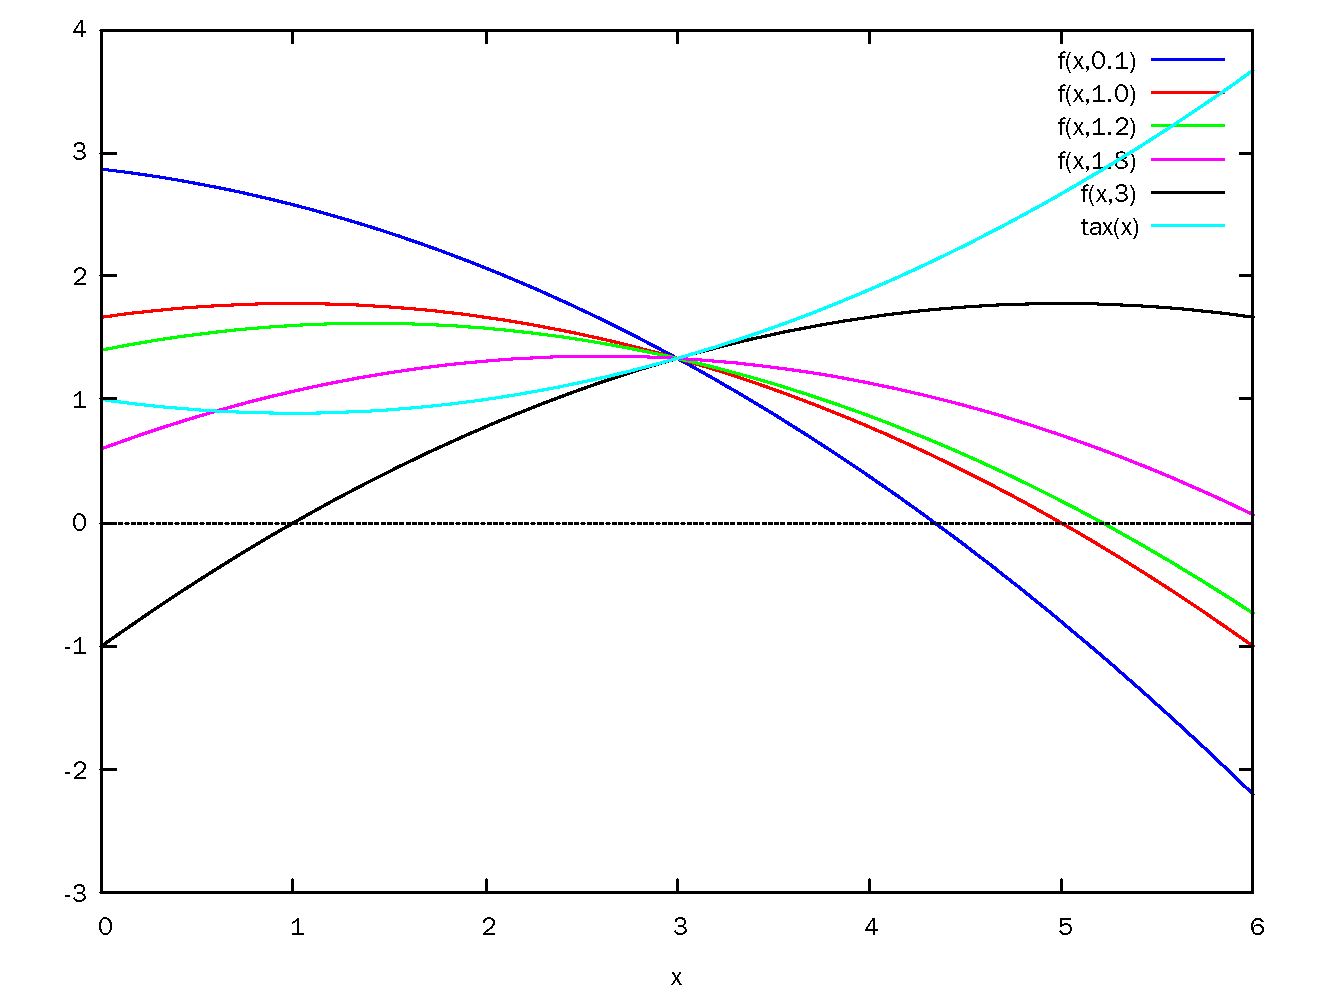
\includegraphics[width = 11cm]{tax.pdf}
\caption{tax scheme $tax(x)$ etc.} \label{fig:tax}
\end{figure}

For this continuously differentiable situation, the private value case of the problem always has the unique solution, the uniqueness
has been shown by the above more general result. And the unique mechanism is the well-known VCG mechanism. This has been shown by
Laffont and Maskin(Econometrica, 1980). 

%And for private value case, 
%ex post implementation is indeed dominant strategy implementation. A specialness of the private value situation is that the calculated
%VCG money transfer mechanism can always satisfy the additional requirement for implementability. We will show why now. 
\section{Discrete social goal}
The discrete social choice possibility set $A$ does not allow differential analysis like we do above in the continuous social choice
possibility set case. However, the allocation of discrete social resources, or the determination of whether a project should be carried
are important social choice problem we have to face. We are also interested at whether we can implement such social choices with money
transfer. We start from allocation of one good.

\subsection{Allocation of one good  }

Imagine the following scenario : there is a group of agents who are familiar with each other, and the social planner has
one good to allocate to one of them. The socially efficient outcome is to give it to the one who 
values it the most. Suppose each agent can only detects one of the qualities of the good, and the total value of the 
good for any agent is only determined by all the qualities of the good and the importance of each quality to the agent 
himself. This is a situation completely covered by our model framework in the previous section. The social choice possibility
set $A=\{(1,0,\cdots,0),\cdots,(0,\cdots,0,1)\}$. Every body only cares about getting the object, and when one does not get it his or
her utility gain is 0 from the allocation. Now what the social planner want is a mechanism to implement the socially efficient outcome. 

\parencite{Maskin00} has partly solved the problem and give us an auction mechanism to implement a rather large economic 
environment set $E$ in this one good allocation environment. However, as the authors pointed out in the footnote 26 of 
their paper, some utility forms can not be implemented by their auction mechanism. In this section, through combining the 
insights of the two authors with the power of revelation mechanism, we try and find a direct revelation mechanism  which
enlarge the $E$ on which the social goal of efficiency $G$ is implementble, for example, the economic environment in footnote
26 of their paper.
In Theorem~\ref{necessary-sufficient}, we have shown what is the sufficient and necessary condition for implementation with money 
transfer. In this simple case, we give some simple assumptions parallel to the sufficient and necessary condition
so that we can implement the social efficiency.

In this one good allocation problem,let $v_i(s)=v_i(\epsilon_i,s)$ where $\epsilon_i$ is the allocation of the good to i. Then we
have the following sufficient condition for ex post implementation of efficient result in an auction.
\begin{prop}
The efficient allocation of one good can be implemented  as an ex post equilibrium
if  
 $$\forall i,\forall s_{-i}, \exists s_i^* \in S_i, such\ that $$
 $$(a) v_i(s_i^*, s_{-i}) = max_{j\not = i} v_j(s_i^*, s_{-i}); $$
 $$(b) When\ v_i(s_i, s_{-i}) > v_i(s_i^*, s_{-i}), $$
  $$\forall j \not = i, v_i(s_i, s_{-i}) - v_i(s_i^*, s_{-i}) > v_j(s_i, s_{-i}) - v_j(s_i^*, s_{-i});$$
  $$When\ v_i(s_i, s_{-i}) < v_i(s_i^*, s_{-i}), $$
  $$\forall j \not = i, v_i(s_i, s_{-i}) - v_i(s_i^*, s_{-i}) < v_j(s_i, s_{-i}) - v_j(s_i^*, s_{-i});  $$
 
\end{prop}
\begin{proof}
The proof is through  constructing the needed mechanism and then examining how the mechanism works in all possible situations.
We only need to find an appropriate mechanism to implement it. Now we give it as follows and then prove it can indeed
 implement the social goal of efficiency.
 
 Step 1. Every agent reports a $(v,s_i)$ from the set $V\times S_i$;
 
 Step 2. If the $v$ reported by every agent has some disagreement, then the result is that no body gets the good.
 
 Step 3. If the $v$ reported by every agent is the same, then solve the maximization problem 
 $$\max_{i \in \{1,\cdots,n\}}v_i(s)$$
 and give the good to the solution agent. The winner pays $v_i(s_i^*, s_{-i})$ 
 which $s_i^*$ is the solution to the following minimization problem
 \begin{equation}
 \min_{s_i^*\in S_i} v_i(s_i^*, s_{-i})\quad
 s.t.\quad  v_i(s_i^*, s_{-i})\geqslant \max_{j\neq i, j \in \{1,\cdots,n\}} v_j(s_i^*, s_{-i})
 \end{equation}\label{pay}
Explanation of this mechanism being able to induce truthful revelation of every agent's private signal is not
difficult with the help of case analysis for all possibilities.

Devide the actually received signal $s_i^*$ into three cases:

(i)When $v_i(s_i, s_{-i})> v_i(s_i^*, s_{-i})$, given others truthfully revealing their private signals $s_{-i}$, the agent i
wishes to win the auction. Truthful revelation of $i$'s private signal is enough to insure the win, since the $s_i^*$
is enough to guarantee a tied first according to assumption (a), further by the first part of assumption (b), the true $s_i$ gives
agent $i$ the clear first. Therefore truthful revelation of the signal $s_i$ in this case is incentive compatible.

(ii)When $v_i(s_i, s_{-i})< v_i(s_i^*, s_{-i})$, given others truthfully revealing their private signals $s_{-i}$, the agent i's best choice is to lose the auction.
Truthful revelation of $i$'s private signal is sure to make him lose the auction, since  the $s_i^*$ only gives him a tied first according to assumption (a), 
further by the second part of assumption (b), the true $s_i$ will not make him the first. Therefore truthful revelation of the signal $s_i$ in this case is also incentive compatible.

(iii)When $v_i(s_i, s_{-i}) = v_i(s_i^*, s_{-i})$, given others truthfully revealing their private signals $s_{-i}$, winning or losing the auction has the same net value of 0. 
Therefore truthful revelation of the signal $s_i$ in this case is incentive compatible trivially.

\end{proof}




The improvement of our mechanism on \parencite{Maskin00} is that they have four assumptions for implementation, but we only need two 
assumptions which are essentially parallel to their first three assumptions and less demanding. 

Their three assumptions are listed below.

(i)$\frac{\partial v_i}{\partial s_i} > 0$;

(ii) $\forall i, j \not = i, \frac{\partial v_i}{\partial s_i}(s_1,...,s_n)
> \frac{\partial v_j}{\partial s_i}(s_1,...,s_n)$,

at any point where $v_i(s_1,...,s_n) = v_j(s_1,...,s_n)= max_k v_k(s_1,...,s_n)$;

(iii)$ \forall s_{-i} \in S_{-i}, \exists s_i' \in S_i, such\ that\ v_i(s_i', s_{-i}) > max_{j\not=i}v_j(s_i', s_{-i})$.


Therefore, we can implement social
 goal of efficiency on all the economic  environments $E$ that their auction mechanism can implement and can implement beyond their
 scope. As a demonstration of the power of our direct revelation mechanism as shown in the proof, we now implement the efficiency 
 goal for \parencite{Maskin00} footnote 26.
 
\begin{example}[Footnote 26 of the paper Efficient Auctions]
$$v_1(s_1,s_2)=s_1-2s_2+5$$
$$v_2(s_1,s_2)=s_2-\frac{1}{2}s_1+5$$
The $v$ clearly satisfy Assumption 1 and 2, therefore it is implementable using our direct revalation mechanism described above. By
using the minimization value in Formula~\ref{pay}, we get the pay that the winner has to make,  which is a constant $5$. It is easy to verify that truthful report is a Nash Equilibrium.
 
\end{example}
For the above example, the reason why the auction in \parencite{Maskin00} cannot implement social goal of efficiency, is perhaps that 
their contingent biding function loses the information revelation role in this case, since 
$b_1(v_2)=15-2v_2,\quad b_2(v_1)=\frac{15-v_1}{2}$.

The next section will be with multiple goods, and there we will provide a sufficient condition for ex post implementation. When that condition is applied to the one object case($1$ is a special case of $n$), we will have a further relaxed condition than the one we proposed in this part.
\subsection{Assignment of multiple goods}
\label{sec:assignment_of_multiple_goods}

For allocation of multiple goods under interdependent value environment, not much has been done to our knowledge. \parencite{Che2015} involve assigning indivisible objects to individuals without monetary transfer under interdependent values setting. Now in this subsection we extend the previous result to the allocation of multiple goods with money transfer under interdependent value environment.  The problem we'll consider is actually the assignment model with a special kind of interdependency. \footnote{For the private value assignment problem, the knowledge of which may help the understanding of this section, see Chapter 8 \parencite{Roth1990}for reference.} 

Suppose that there are $m$ agents and $n$ goods such that $m > n$. Each agent can get at most one object.   Agent $i$'s valuations of the n goods is given by $(v_{i1}(s),v_{i2}(s),...,v_{in}(s))$ respectively, where $s=(s_1,s_2,...,s_m)$ is a vector of signals held privately by agent $1$,agent $2$,..., agent $m$ respectively. Allocation result is a $m \times n$ matrix $X$ where $\sum_{i\in\{1,...,m\}}x_{ij} \leq 1 \text{ for all } j$ and  $\sum_{j\in\{1,...,n\}}x_{ij} \leq 1 \text{ for all } i$. The social goal is to allocate the goods to maximize the social efficiency $\sum_{ij}x_{ij}v_{ij}(s)$.

This problem is generally not ex post implementable. However, we find under the following condition, we can design a mechanism to implement the socically efficient goal in ex post equilibrium.

Condition $\rho$:

$\forall i,\forall s_{-i}, \exists s_i^*$,for all $k \in \{1,\cdots,n\}$, such that :

from the maximizing solution $x$s to  $\sum_{ij}x_{ij}v_{ij}(s)$, one can designate an allocation scheme, such that

%if $s_i = s_i^*$, agent $i$ will be given the certain good $k$ or have no good allocated in a value maximizing allocation schemes.

if $v_{ik}(s_i) < v_{ik}(s_i^*)$, agent $i$ will have no probability to be allocated the good $k$. %in all the maximizing allocation schemes.

if $v_{ik}(s_i) > v_{ik}(s_i^*)$, agent $i$ will have a probability to be allocated the certain good $k$ and charged $ v_{ik}(s_i^*)$. However, the probability does not depend on $s_i$. % in all the maximizing allocation schemes.


\begin{proof}
  The proof is through  constructing the needed mechanism and then examining how the mechanism works in all possible situations.
  
We first need to find an appropriate mechanism. Now we give it as follows and then prove it can indeed implement the social goal of efficiency.
 
 Step 1. Every agent reports a $(v,s_i)$ from the set $V\times S_i$.\footnote{Here $v$ is the matrix
   \begin{matrix}
     v_{11}& \cdots & v_{1n}\\
     \vdots& \ddots & \vdots\\
     v_{m1}& \cdots & v_{mn}
   \end{matrix}
   , where $v_{ij}$ is the value function of agent $i$ getting good $j$.
 }
 
 Step 2. If the $v$ reported by every agent has some disagreement, then the result is that no body gets any good.
 
 Step 3. If the $v$ reported by every agent is the same, then to allocate the goods, choose the social value maximizing allocation scheme designated in Condition $\rho$ which satisfy the additional two assumptions in it.
 
 
 
 
Explanation of this mechanism being able to induce truthful revelation of every agent's private signal is not
difficult with the help of case analysis for all possibilities.

For any $k$, devide the actually received signal $s_i$ into three cases:

(i)When $v_{ik}(s_i, s_{-i})> v_{ik}(s_i^*, s_{-i})$, given others
truthfully revealing their private signals $s_{-i}$, the agent i
wishes to be assigned good $k$ to gain $v_{ik}(s_i, s_{-i})- v_{ik}(s_i^*, s_{-i})$ surplus. Truthful revelation of $i$'s private signal gives $i$ a probability of the assignment of $k$ to $i$, since $s_i$ will not influence this probability,
truthful revelation of the signal $s_i$ in this case is incentive
compatible.\footnote{Not influencing probability is important, because if not, agent $i$ would have incentive to manipulate the probability by report a false $s_i$.}

(ii)When $v_{ik}(s_i, s_{-i})< v_{ik}(s_i^*, s_{-i})$, given others
truthfully revealing their private signals $s_{-i}$, the agent i wishes not to be allocated the good and being charged
$v_{ik}(s_i, s_{-i})< v_{ik}(s_i^*, s_{-i})$. Truthful
revelation of $i$'s private signal $s_i$ is enough to insure that he
is not allocated good $k$ by Condition $\rho$.  truthful revelation
of the signal $s_i$ in this case is also incentive compatible.

(iii)When $v_{ik}(s_i, s_{-i}) = v_{ik}(s_i^*, s_{-i})$, given others
truthfully revealing their private signals $s_{-i}$, winning or losing
the assignment of good $k$ has the same net value of 0. Therefore
truthful revelation of the signal $s_i$ in this case is incentive
compatible trivially.

Therefore, truthful revelation is incentive compatible overall for this mechanism.

\end{proof}

Condition $\rho$ does not seem to be easy to satisfy. Nevertheless, in
the following we give a more concrete $v$ which satisfy Condition
$\rho$ to show that it is indeed satisfiable in some situations so
that we can ex post implement the socially efficient goal.
\begin{prop}
  \label{rho}
  The social efficient goal of $\max_{x}x_{ij}v_{ij}(s)$ can be ex post implemented if:
For all $i$ and $j$,
$$v_{ij}=b_{ij} + o_i(s_i) + \sum_{l \not = i} r_l(s_l) $$
where $b_{ij}>0$ is the base value, $s_i \in [0, + \infty)$, $\forall i,o_i(0)=r_i(0)=0$

Assumptions are listed below.

(i)For all $i$, $\frac{\partial o_i}{\partial s_i} > 0$, $\frac{\partial r_i}{\partial s_i} > 0$;

(ii) $\forall i, \frac{\partial o_i}{\partial s_i}
> \frac{\partial r_i}{\partial s_i}$;

%(iii)Faced with a $s_{-i}$, as the $s_i$ increases, agent $i$ will finally get some good allocated in the solution of the assignment problem.
\end{prop}


The intuition of these assumptions implying Condition $\rho$ is that
the own effect of a signal $s_i$ is larger than its effect to the rest
of the agents. And therefore there exists a threshold $s_i^*$ as
required by Condition $\rho$ for agent $i$ to get into the group of
good winners. As for the fixedness of the good winning probability by agent $i$,
it's in part due to the fact that as $s_i$ increases, the increasing
rate of $v_{ik}$ is at least as large as any other $v_{ab}$, where
$ab$ stands for arbitrary agent and good combination not equal to
$ik$. The formal proof can be seen in Appendix \ref{Appendix_C}.







\section{Conclusion}

We have focused on designing mechanisms implementing social goals truthfully in ex post equilibrium. The one caveat is that there may be collusions among the players. The way to deter this is to form laws against such behaviors globally or to negotiate on contracts against such behaviour locally. Why not just form laws against lying and save all the efforts of designing incentive compatible mechanisms ? The answer is that lying by a person is much harder to detect than collusion by a groups of people, and we can hardly penalize lying with law due to lackness of concrete evidence.

The whole chapter builds on the assumption of quasilinearity of agents' value function. Under such preference,  money can be utilized 
as a tool to help elicit true information about the world that are scattered among the agents.
When the mechanism designer cares more on efficiency than fairness, our mechanism is ideal. Since the redistributional effect of money 
transfer has no influence on the aggregate social value.

%----------------------------------------------------------------------------------------




%----------------------------------------------------------------------------------------


% Chapter 4

\chapter{Matching}  % Main chapter title

\label{Chapter4} % For referencing the chapter elsewhere, use \ref{Chapter4} 

%----------------------------------------------------------------------------------------

% Define some commands to keep the formatting separated from the content 
%\newcommand{\keyword}[1]{\textbf{#1}}
%\newcommand{\tabhead}[1]{\textbf{#1}}
%\newcommand{\code}[1]{\texttt{#1}}
%\newcommand{\file}[1]{\texttt{\bfseries#1}}
%\newcommand{\option}[1]{\texttt{\itshape#1}}


\section{Introduction to the basic concepts}



%I would like to introduce Coq Proof Assistant for this purpose, 
% for there are many theorems in matching theory which can be proved
% more strictly and without errors with its help. My motivation comes
% from the fact that proof error is easy to creep into human proofs 

% and most proofs can only be best understood and checked by the original author when the body of theorems and propositions in matching theory become more and more abstract in quality and large in
% quantity. 
 
% The adoption of Coq for this subject is an idea inspired by the 2002 Fields Medal Winner Vladimir Voevodsky's recent project Univalent foundations for mathematics. He uses Coq to formalize the proofs of theorems
% in homotopy theory and try to build another foundation of mathematics which can be viewed as equal to the set theory but is much easier for the computer to check the correctness of proofs. 
 
% first, we consider the easy one. Man woman marriage market as defined in the classical work of (Alvin Roth and SotoMayor). 
% We define these markets as a type with m men and n woman as follows
% Inductive Market (m n: nat) :=
% |mkt: Men n -> Women m -> Market m n
We consider two-sided matching in this chapter. There was a monograph dedicated to it, see \parencite{Roth1990}. However, we will focus on application of the theory to Chinese college admission mechanism, and use some notions that have recently developed. In this section, some of the most important theoretical concepts and results are introduced. 

In two sided matching, the two
distinguishable sides of matching are assumed to be men and women,
students and schools, workers and employers, tenants and houses,
etc. Here, students and colleges are chosen as the economic
background. For this specific topic, there
is \parencite{Sonmez2003}  which give a description of the literatures
in this field till that time. 

Now A description of the model and relevant notations that will be used in this chapter. There is a finite set of students and a finite set of colleges denoted by  $S = \{1,...,n\}$ and $C = \{1,...,m\}$, respectively. For any $j \in C$, college $j$ has $q_j$ quota, which is college $j$'s seats for students. Students wish to enter at most one college and have an option not to enter any college at all. This outside option is formally represented by a null college, denoted by $0$. This null college has unlimited quota, ie, $q_0 = + \infty$. 

A matching(sometimes also called assignment or allocation) is a
mapping $\mu : S \rightarrow C\cup\{0\}$ such that for any $j \in C$,
$|\mu^{-1}(j)| \leq q_j$. Denote by $\mu(0)$ the set of colleges with
seats that is not assigned to any student at matching $\mu$. The null
college is always included in this set, as its seat supply is
unlimited. Hence:
\[ \mu(0) = \{j \in C : |\mu^{-1}(j)| < q_j\}\cup \{0\}\]


We assume that students have preferences on colleges.  Denote by $R_i$ student $i$'s preference on the set of colleges $C \cup \{0\}$. The corresponding strict preference and indifference relations are denoted by $P_i$ and $I_i$, respectively. The meaning of the notation is as follows: if $c,c'\in C \cup \{0\}$ and $c R_i c'$, then student $i \in S$ weakly prefers college $c$ to college $c'$. Change ``weakly prefers'' to ``strictly prefer'' we get the meaning for the strict $P_i$. Change ``weakly prefers'' to ``are indifferent'' we get the meaning for the indifferent $I_i$. Preferences are assumed to be rational in the sense that for all $i \in S$, $R_i$ is complete, reflexive and transitive. A preference profile is a list $ R = (R_1,...,R_n)$ of the students' preferences. All the discussions here and after are based on the strict preference assumption. That is , if $c I_i c'$, then $c=c'$.\footnote{Because the students have strict preference, a college can only be indifferent to itself in any student's preference. No two things are exactly the same, and indifference are usually the result of inadequate information, so here we assume aspects of the university are known to the extent that the colleges can be ranked by a student.}

 Here, a priority structure $\pi$ is assumed for the colleges, that is, for each college $j \in C$, there is an exogenously given strict priority-order $\pi_j$. Formally, $\pi_j: S \rightarrow \{1,\cdots,n\}$ is a bijection where the highest-ranked student  is the student $i\in S$ with $\pi_j(i)=1$, the second highest ranked student $i' \in S$ has $\pi_j(i')=2$, and so on. When $\pi_j$ is the same for all $j\in C$, we get the serial dictator matching mechanism. A priority structure is a list $ \pi = (\pi_1,...,\pi_m)$ of the colleges' priority-order. For the concept of pairwise stable, this priority structure is enough. \footnote{For group stable or core, further definition of college preference on groups of students should be provided. And for substitutable college preferences which is an implied assumption of this chapter, the two concepts coincide. See Proposition 6.4 in \parencite{Roth1990} for more details.}

 A matching $\mu$ is pairwise stable(or called priority respecting as in \parencite{Svensson2014}) if there is no student $i \in S$ who strictly prefers some college $j$ to $\mu(i)$ and $\mu^{-1}(j)$ contains some other student $i' \in S$ who has lower priority for college $j$ than student $i$(i.e., $\pi_j(i')>\pi_j(i)$), and furthermore, all students weakly prefer their assigned college seats to any unassigned seats in $\mu(0)$(seats from the same college are obviously equal). We'll simply use stable to mean pairwise stable later in the chapter.

 Formally ,the definition of stableness is as follows.

\begin{definition*}(stableness)
A matching $\mu$ is stable for a given preference profile $R$ and a given priority structure $\pi$, if :

(i) for all $i,i' \in S$, $\mu(i')P_i \mu(i)$ only if $\pi_{\mu(i')}(i') < \pi_{\mu(i')}(i)$;

(ii)for all $i \in S$, $\mu(i)R_i j$ if $j \in \mu(0)$, where $\mu(0) = \{j \in C : |\mu^{-1}(j)| < q_j\}\cup \{0\}$.

\end{definition*}

Condition (i) is called fairness condition, with the meaning that
there is no justified envy\footnote{justified envy means that you envy somebody
else's college and according to your priority in that school, you
should be admitted prior to that person}. Condition (ii) is the combination of
individual rationality and non-wastefulness. Rationality means that
the current assignment of college for a student must be weakly better than the outside
option of null college 0. Non-wastefulness means that the current
assignment of college for a student  must be weakly better than any
unocuppied college seat. For more detailed discussion of these concepts
, see also \parencite{Sonmez1999}. 

The next important concept is Pareto efficiency for students or simply
efficiency. A matching is pareto efficient if no other matching can
make at least one student get a strictly more preferred college while
no student get a strictly less preferred college. 

Formally, we have the following definition.
\begin{definition}
A matching $\mu$ is efficient for a given preference profile $R$, if
for all $\mu'$ such that there exists $i \in S$ satisfying $\mu'(i)
P_i \mu(i)$, then there must be some other $i' in S$ satisfying
$\mu(i') P_{i'} \mu'(i')$
\end{definition}

It is clear that efficiency for students does not take into account of college priority while stableness does need it. Stableness is priority respecting and includes a flavor of fairness in it. Now that we have some idea about matching, we begin to investigate mechanism that can lead to stable and efficient matching. An important difference between matching mechanism design and other mechanism design such as auction is that efficiency is usually not the only requirement, stableness or priority respecting is at least of equal importance. We will illustrate this later in examples.

Why do we care about priority? In the previous chapter, we only care about efficiency. which means to maximize the sum of all participants' utilities. However, there is a well known saying that the whole is more than the parts put together. Priority should belong to the more-than part of the whole. suppose that only students entering their most preferred college will study hard, and any student would feel the same level of happiness when they enter their most preferred college but those with high scores will contribute more to the society, so high scored students should have priority. However just by the limited maximizing sum efficiency criterion we would send arbitrary student to their most preferred college, while from the society as a whole giving the high scored students high priority is a better choice.\footnote{I never believe this myself, so it is only a possible reason coined to show that priority may matter to the social welfare; other possibility of it may be fairness itself is an component of social happiness.}

When it comes to mechanism design, the usual problem of unilaterally misreporting one's private information(here is one's preference) emerges. In the literature, a mechanism that is immune to such problem is often called strategyproof. Viewing the reporting of one's preference under a mechanism as a game among the students, strategyproofness  means that it is a dominant strategy to report one's true preference. 

There is also a related concept called group-strategyproof. What is the connotation of this concept? It means that no group can get a pareto improvement by unilaterally changing the reports of students in this group under the mechanism. Viewing the reporting of one's preference under a mechanism as a game among the students, group-strategyproofness means that it is a core equilibrium for everyone to report the private true preference.



\section{Popular matching mechanisms}
\label{equivalent direct mechanisms}
There are many matching mechanisms. Three kinds are
most studied. They are the Deferred Acceptance Mechanism(DA), the Top
Trading Cycle Mechanism(TTC), and the serial dictatorship mechanism(SD).
These three mechanism are all related to the later analyzed Chinese
student-college matching mechanism, especial the DA mechanism. Why are they most popular? 
One reason is that all of these mechanisms are
strategyproof. Therefore the reported preference profile are true preferences
for rational agents.

Among these, DA mechanism is what will be of key importance in the later modelling and discussion of Chinese college admission
mechanisms. Thus an indepth investigation is provided in the following subsection.



\subsection{Deferred Acceptance Mechanism}
In the seminal work \parencite{Gale1962}, DA mechanism is first
proposed. This mechanism is the first and probably the most studied
mechanism in modern matching theory. 

In the setting of student-college matching, it is also called
student-optimal stable mechanism (SOSM) for it always finds the stable
matching that is most favorable to each student. Its outcome can be
calculated via the following Deferred
Acceptance (DA) algorithm for a given problem:

 Step 1: Each student applies to his or her favorite school. For each
college $j$, up to $q_j$  applicants who have
the highest college $j$ priority are tentatively assigned to college $j$. The remaining applicants are
rejected.

Step k ($ k \geq 2$ ): Each student rejected from a college at step k -1 applies to her next favorite college.
For each college $j$, up to $q_j$  students who have the highest college
$j$ priority among the new applicants and those tentatively on hold from an earlier step, are
tentatively assigned to college $j$. 
The remaining applicants are rejected.

The algorithm terminates when no student applies to any new college in
some step. That is, every  student is either tentatively placed to a college
or has been rejected by every college that is better than null college
in his or her preference list. 

We list important properties concerning the DA mechanism here.

Under strict priority( that is, no two colleges have  the same utility
level for a student.), the following properties
hold. \parencite{Gale1962} first proposed the two theorems and proved
them. The proofs for the theorems are short and elegant, and therefore
provided in Appendix \ref{Appendix_D}.

\begin{thm*}(Gale-Shapley)
The matching given by DA mechanism is stable.
\end{thm*}

\begin{thm*}(Gale-Shapley)
Every student is at least as well off under the assignment given by
the DA mechanism as he would be under any other stable assignment.
\end{thm*}

These two theorems can be combined into one concise statement. The SOSM
matching produced by the DA mechanism is the optimal stable matching.
An alternative way to express this is that if you want to find a
matching that is stable, the SOSM matching selected by the DA  mechanism is the most
efficient matching(constrained efficiency).

\begin{thm*}
\label{thm1}
The DA mechanism is strategy-proof for the students.
\end{thm*}

The proof of it is complex and need more notions, please see \parencite{Roth1982a} or \parencite{Roth1990}for proof.
However, the DA mechanism is not pareto efficient.  This fact can be shown by an example.

\begin{example}
There are two colleges $A$ and $B$, each with 1 seat for students. A null college $0$ with unlimited seats and accepts who ever applies for it. There are
3 students 1,2,3. The preferences of the students are
as follows.

    \begin{center}
      \begin{tabular}{|c|c|c|}
        \hline
        $1$ & $2$ & $3$ \\
        \hline
        $A$ & $B$ & $A$ \\
        
        $B$ & $A$ & $B$ \\

        $0$ & $0$ & $0$ \\

        \hline
        
      \end{tabular}
    \end{center}

The two colleges' base priority structure is the same as in the following
table

 \begin{center}
      \begin{tabular}{|c|c|}
        \hline
         $A$ & $B$ \\
        \hline
        $2$ & $1$\\
        
        $3$ & $3$ \\

        $1$ & $2$ \\
       
        \hline
        
      \end{tabular}
    \end{center}
 
The DA mechanism is run round by round as in the table below.

 \begin{center}
      \begin{tabular}{|c|c|c|c|}
        \hline
        &$1$ & $2$ & $3$\\
        \hline
       round1&   & $B$ & $A$ \\
        
        round2&$B$ &  & $A$ \\

        round3&$B$ & $A$  & \\

        round4&$B$ & $A$ & $0$\\
        \hline
        
      \end{tabular}
    \end{center}

Because 3 is the only student not tentatively accepted after 3 rounds,
and 3 has been rejected by both A and B, the DA algorithm with quota
terminates with student 1 entering B, 2 entering A, and 3 entering null college $0$.

Now consider the following alternative preference profile.
\begin{center}
  \begin{tabular}{|c|c|c|}
    \hline
    $1$ & $2$ & $3$ \\
    \hline
    $A$ & $B$ & $0$ \\
    
    $B$ & $A$ & $A$ \\

    $0$ & $0$ & $B$ \\

    \hline
    
  \end{tabular}
\end{center}

With this profile, the DA mechanism is run as below.

\begin{center}
  \begin{tabular}{|c|c|c|c|}
    \hline
    &$1$ & $2$ & $3$\\
    \hline
    round1& $A$  & $B$ & $0$ \\
    
    \hline
    
  \end{tabular}
\end{center}

Just 1 round, and the DA process is terminated.





\end{example} 

\begin{remark}
 If a mechanism is able to produce every possible matching results, then not pareto efficient obviously means that the mechanism is not group-strategyproof, since reporting the profile that can result in a pareto improvement assignment is a profitable group-deviation.
\end{remark}


%\subsection{Top Trading Cycle Mechanism}
%This mechanism is given in \parencite{shapley1974}. It is also an
%important mechanism and being studied and modified by scholars across
%the matching area since 1974 

%In the student-college matching setting, the TTC matching result is
%determined after the following process.


%\subsection{Serial Dictatorship Mechanism}

\section{Analysis of Chinese college admission mechanisms}

As an application of the matching theory, we will focus
on the Chinese college admission mechanisms in this section.

The Chinese college admission is a centralized matching mechanism with
an entrance exam taken national wide as a means of student-priority
deciding tool for the colleges.
Students from high school in China need to take an entrance exam to
decide the student priority for colleges, and the priority structure
is also influenced by the application form that the students write to
inform authority their own preferences. The college entrance exam, or Gaokao in Chinese Pinyin,  forms the 
foundation of the priority determination process for the current
admission system. However,the stage of priority determination through examimations is not the concern of us. There is a complication in the real system, the colleges are classified into batches, where each batch of colleges share the same enrollment scoreline, that is, the minimum score that a student must have in order to be considered eligible for colleges of that batch. However, Shanghai has first abandoned the classification of colleges into batches with different enrollment scoreline from 2016, and many other provinces have anounced their plan to reduce batches or simply abandon batches since then. This complication is not considered in our analysis.

We are interested in mechanisms about how to match the college and students once the priority has been determined. Starting from the early 1950s,
the mechanisms adopted for the stage of matching has gone
through series of reforms,  and what kind of mechanism should be adopted is
currently still in debate. There are millions of high school seniors compete
for  seats at various colleges and universities in China each
year. The matching of students to these colleges and universities has
profound implications for the education and labor market outcomes for
these students.  The fairness and efficiency of this matching process,
is of great importance to the society.

Many Chinese scholars have writen articles discussing problems related
to Chinese college admission mechanisms. \parencite{Zhong2004} has investigated the effects
of three preference report timings on the efficiency of the final matching, i.e. reporting preference
before the exam, after the exam but not knowing the exact scores,  and
after the scores are known.  This study has focused on the
strategical interaction of students in the games, not on how to induce
the truthful reporting with a suitable matching mechanism later in the match stage.  As to the strategical importance of
preference reporting,  Haifeng Nie has written many articles.  Both \parencite{Nie2007a}
and \parencite{Nie2007b} has stressed the point that a good score may
not be as useful as a good strategy for reporting the preference of
the university. This somewhat strange phenomenon has motivated us
in studying the issue of reducing manipulation and inducing better
and fairer results.

The Chinese  matching mechanisms has also recently caught attention of overseas scholars from
the economic field of matching. \parencite{YanChenJPE} has
done much to analyze theoretically the sutleties of the different
mechanisms adopted, and has gone even further to design experiments
for studying features of these mechanisms,
see \parencite{YanChen2016}. Though much has been investigated by them, we still find something interesting in addition to what they find.



\subsection{A simple characterization of the popular matching mechanisms in CCA}

The mechanisms are hard to analyze with all the real application-rejection procedures mixed in the definition,
so we will deal with the equivalent direct mechanisms of the mechanisms actually in use.

When studying ex post equilibrium results for existing
mechanisms which are not direct revelation mechanism, we will convert it to aa
equivalent direct revelation mechanism with the same matching results for expositional convenience\footnote{We put the
  mechanisms in the same revelation mechanism class. and this make it easier to do
  comparison.}  Also to aid analysis and exposition, a notion of successful
manipulation which means a best report choice given others' reports is
used in later analysis of the strategical interaction of
students in the CCA matching mechanisms. \footnote{ It is
  essentially the best response concept in Nash equilibrium but sounds
  more fluent when used in description of the strategical interactions
  among the students.}

Now, let's introduce three important class of mechanisms: DA mechanism, IA\footnote{Immediate Acceptance mechanism, also known abroad as the Boston Mechanism for its adoption in Boston district, uses the same accept-reject procedure as DA, only the acceptance is not tentative but final.}
mechanism and parallel mechanisms. DA mechanism is what we have investigated in the previous section, but it has never been truely adopted in China
due to the fact that the length of reported preference list is too small a number compared to the hundreds of colleges. The Immediate Acceptance (IA)
mechanism  had been the main mechanism used in Chinese
student assignments both at the high school and college
level \parencite{Nie2007b}. However, this mechanism has a serious
limitation: “a good score in the college entrance exam is often worth less
than a good preference reporting strategy” \parencite{Nie2007a}. In our paper's wording, a successful
manipulation is often more important than your score level. This
problem arises from the special priority structure in the
mechanism. Priority of a student in a college is based on the
reported preference list firstly and based on your scores secondly, a
dictionary order that put too much emphasis on preference
reporting. Given in \parencite{Nie2007b}, and also cited
in \parencite{YanChenJPE}, one parent has the following explanation of
the problem.

``My child has been among the best students in his school and school district. He
achieved a score of 632 in the college entrance exam last year. Unfortunately, he was
not accepted by his first choice. After his first choice rejected him, his second and third
choices were already full. My child had no choice but to repeat his senior year.''

To alleviate this problem of high-scoring students not being accepted by any universities, the
parallel mechanism was proposed. 
In the parallel mechanism, students select several
“parallel” colleges within each choice-band. The priority structure is changed. A detailed description from \parencite{YanChenJPE} is cited here for your full understanding of the mechanism.

``a student’s first choice-band may
contain a set of three colleges, A, B, and C while her second choice-band may contain another set
of three colleges, D, E, and F (in decreasing desirability within each band). Once students submit
their choices, colleges process the student applications, using a mechanism where students gain
priority for colleges they have listed in their first band over other students who have listed the same
college in the second band. Assignments for parallel colleges listed in the same band are considered
temporary until all choices of that band have been considered. Thus, this mechanism lies between
the IA mechanism, where every choice is final, and the DA mechanism, where every choice is
temporary until all seats are filled.''

In 2003, Hunan fisrt implemented the parallel mechanism, allowing 3
parallel colleges in the first choice-band(or called group), 5 in the second choice-band, 5 in the third choice-band, 5 in the fourth choice-band, and so on, see \parencite{YanChenJPE}.  The parallel mechanism is soon to be widely perceived as having improved allocation outcomes for students. Citing a parent from a newpaper report \footnote{Li Li. “Ten More Provinces Switch to Parallel College Admissions Mechanism This Year.” Beijing Evening News,
June 8, 2009.},

``My child really wanted to go to Tsinghua University. However,  in order not to
take any risks, we unwillingly listed a less prestigious university as her first choice.
Had Beijing allowed parallel colleges in the first choice band, we could at least give
Tsinghua a try.''

%However, I would like to describe all the three mechanisms
 %as generalized DA mechanisms with different priority structures.
In the paper \parencite{YanChenJPE}, they have formulated the IA
mechanism, parallel mechanisms, and DA mechanism as a parametric family
of application-rejection mechanisms. In this chapter, they are all
converted to their equivalent direct mechanisms. The following are the definitions.

\begin{definition*}direct revelation DA mechanism:
  
Each student reports his or her preference list, each college reports its priority criteria(usually scores plus some tie-breaking rules),then after collecting all these preference lists and priority criteria, the social planner runs the DA procedure
to produce a final matching result.
\end{definition*}

\begin{definition*}direct revelation IA mechanism:

Each students reports his or her preference list, each college reports its priority
criteria(usually scores plus some tie-breaking rules),then after
collecting all these preference lists and priority criteria, the
social planner adjusts the priority rule such that the reported
priority criterion of a college is made only a tie-breaking rule, and the rank of a college in a student's reported preference list is
the main priority criterion. Finally,
the social planner runs the DA procedure
to produce a final matching result.
\end{definition*}

The parallel mechanisms are a wide group of mechanisms. Therefore we need to devise a group of equivalent direct mechanism for them all. However,
parallel mechanisms only differ in the choice-band sizes, so different list of choice-band sizes characterizes a different parallel mechanism.

\begin{definition*} characteristic list of a parallel mechanism:
  
  An infinite list of integers greater than zero $(e_1,e_2,\cdots)$ is the characteristic list of a parallel mechanism if the $e_1,e_2,\cdots$
  define the choice-band sizes for the 1st ranked, 2nd ranked, $\cdots$  choice-bands.
\end{definition*}

Henceforth, a parallel mechanism with a characteristic list $(e_1,e_2,\cdots)$ will just be called mechanism $(e_1,e_2,\cdots)$.


\begin{definition*}direct revelation parallel mechanism $(e_1,e_2,\cdots)$:

  Each student reports his or her preference list, each college reports its priority
  criteria(usually scores plus some tie-breaking rules). After
  collecting all these preference lists and priority criteria, the
  social planner uses the preference list to produce a list of college
  choice-bands according to the characteristic list $(e_1,e_2,\cdots)$
  such that the 1st ranked choice-band
  includes the top $e_1$ colleges in the preference list, the 2nd
  ranked choice-band includes the top $e_2$ of the remaining colleges in the preference list, and so on. Then the social planner adjusts the
  priority rule such that the reported priority criteria of a college
  is made only a tie-breaking rule, and the rank of the choice-band
  which a college belongs to in a student's reported preference list
  is the main priority criterion. Finally, the social planner runs the
  DA procedure to produce a final matching result.
\end{definition*}

These three direct mechanisms are henceforth just called DA, IA and parallel mechanisms.
From the definition of parallel mechanisms, we can see that DA and IA mechanisms are two special forms of parallel mechanisms with characteristic
list $(+\infty,0,0,\cdots)$ and $(1,1,1,\cdots)$. Therefore they can also be called mechanism $(+\infty,0,0,\cdots)$ and mechanism $(1,1,1,\cdots)$.





The IA mechanism and parallel mechanism are qualitatively different from DA. Their
priority structure are closely related with the reported preference
while the priority structure of DA has no connection with the reported
preference. The underlying idea for the IA mechanism or parallel mechanisms is
``Colleges should like those who like them''.  This is exactly where manipulations creep
in.  

Formally, under the setting of student-college matching, we have the following definition.

\begin{definition}
A mechanism of matching is non-manipulable, if given any preference
$R$, and priority structure $\pi$, $\mu = h(R, \pi(R))$ and for any $i
\in S$, denote $h(R_i',R_{-i}, \pi(R_i',R_{-i}))$ by $\mu'$, then we have $\mu(i)R_i \mu'(i)$.
\end{definition}

We have the following claim.
IA and parallel mechanisms are manipulable. DA is non-manipulable.
Its proof can been found in \parencite{YanChenJPE}.
 
\begin{remark}
The efficiency and stableness concept is apparently not very useful when
the reported $R$ is not true. What we should be concerned is the status of the matching
result in the perspective of true $R$. So we have investigated the manipulability first.
\end{remark}

Because manipulation exists, investigating the matching result to the reported preference is of little meaning for the true social welfare. Therefore matching theory about the property of matching results to the reported preference is not applied in investigating Chinese college admission mechanisms. Without strategyproofness, we have to find another equilibrium solution concept other than dominant strategy equilibrium to study the likely matching results.

In this section we would like to view the mechanisms from a perspective of ex post Nash equilibrium.
Here, the ex post should not be taken 
literally, it does not mean that 
evaluating the action after some particular time. Actually, it means that assuming that every action and information of the other players have been known, the player still insists on his choice due to its optimality with respect
to the others' actual action or choice. In fact, it may happen that the player will never know all the actions of the other players and therefore there is not a time point after which all information is revealed. 
The important thing is that the action or manipulation can be called successful when all information and actions are known.
Formally, we give the following definition in the college admission setting. 
\begin{definition}
A student i has a successful report 
if let $R$ denote the true preference, $R'$ the reported preference, $\mu' = h(R')$, then for any $R_i''$, let $\mu''= h(R_i'',R_{-i}')$, we have  $\mu'(i) R_i \mu''(i)$
\end{definition}

We extract this concept from the definition of ex post Nash equilibrium. It is in fact a component of ex post Nash Equilibrium. An ex post Nash equilibrium is just where all agents have successful reports simutaneously. 


In this chapter, We consider deterministic game forms and only consider pure strategies. Our ``ex post'' concept requires that the strategies to be considered must be pure because you cannot report this preference and that preference at the same time when every thing is known\footnote{Only scholars who study quantum games may have disagreement. However,we do not consider quantum games here.}.

From the social point of view, the ex post equilibrium with every player successfully reports is in a sense the fairest result that a mechanism can have. In an ex post equilibrium, no body has done worse because of lack of information\footnote{Disparity of information acquisition is a very important source of unfairness}.


We will show that in the Chinese style college admission, the IA mechanism, the parallel mechanisms and the DA mechanism have the same matching result in their expost equilibrium. However, it is not 
easy to achieve the expost equilibrium for the IA mechanism and the parellel mechanism because they need lots of information to achieve it but the informtion is not easily acquired. On the contrary, the DA's ex post equilibrium can be achieved just by every player reporting the true preference, and it is indeed a dominant strategy equilibrium, stronger than merely an ex post equilibrium.

Now a definition that is useful in formally expressing the ideas in the previous paragraphs.
\begin{definition}
under a preference reporting direct mechanism $h(.)$, students report some preference profile $R$, then the matching result is $\mu=h(R)$.
If all students have successful reports in this case, then the matching result $\mu$ is an ex post equilibrium outcome, and called achievable with perfect manipulation under the mechanism $h(.)$.
\end{definition}

There is a difficulty in analysing the true welfare property of a matching outcome achievable with perfect manipulation under a mechanism. The difficulty is that  even if you know that in the ex post equilibrium the matching result
is successfully manipulated by everyone, you do not know if it
satisfies a social goal $f(R)$, because you do not know the true preference $R$ in the economic
environment because of manipulation of preference reporting!


In \parencite{YanChenJPE}, they started analysis of parallel mechanisms with the symmetric parameter setting, i.e., $e =e_1=e_2=\cdots$ before studying the general case where $e_1, e_2,\cdots$ might be unequal parameters. In the general case, they proved a nested manipulability structure for parallel mechanisms, and then they paid attention to stability comparisons between parallel mechanisms with an additive decomposition relationship. However, for ex post equilibrium outcomes, they only give the Proposition 4 in the symmetric parameter setting. As a new contribution, we find a nested structure of the ex post equilibrium outcomes in parallel mechanisms, and have proved that the set of ex post equilibrium outcomes is only related to $e_1$ but not influenced by $e_2,e_3,\cdots$.   





 Before diving into the case of general priority structure, we first
focus our attention on a very important kind of priority structure,
the score-based priority structure and discuss what kind of matching
results can be achieved with perfect manipulation under such uniformly
score-based priority. This interest comes from reality. In CCA, the priority criteria is basically the scores with some similar tie-breaking rules across colleges, and the examination paper is usually the same nationwide\footnote{Only Beijing, Shanghai, and a few provinces choose to devise an exam paper of their own} .

DA mechanism just use the score high-low comparison to determine
priority of students for every college. The more score you get, the
high priority you get.

As to the adjusted priority structure in IA and parallel mechanisms, it is described as following.
To determine a student $i$'s priority in college $j$, parallel
mechanism fisrt group the colleges according to $i$'s reported
preference list. For example, in Tibetan's parallel mechanism, every
group has 10 colleges, then you group the first 10 together and label
every college in this Group 1, group the second 10 together and label
every college in this Group 2, and so on. A student's priority in a
college is determined in a dictionary order. First, compare the group
number of the college for the student. For instance, if Beijing
University is in the first 10 college group for a tibetan student, 
then this student has a higher priority in Beijing Unversity than
tthose who has not put  Beijing University in the first 10 college
group. If two students put the college in the same Group $n$, then
comes the second procedure of comparison. The student with higher
score(or high original priority) has higher priority. IA mechanism is
just a parallel mechanism with every group size equal to $1$.

In fact, the important thing is not that the priority structure is score-based nationwide, but that it is the same across colleges.
We have the following important theorem.

% and only modify the priority structure as described for the IA and parallel mechanism,
\begin{thm}\label{same}
If every college has the same base priority for the students, then the matching achievable with perfect
manipulation,that is, the ex post equilibrium matching result,  under the IA and parallel mechanism  is the same with the one under the DA mechanism, which is unique , stable and constrained efficient. 
\end{thm}

%In this section, we would like to show
%that the matching results that can be achieved with perfect
%manipulation is the same with the truthful revelation matching under the corresponding
%DA that results from deleting the adjustment that was done to the colleges' reported priority structure.\footnote{We do not consider college's
% strategic behaviour or preference, that is, we just view the report of colleges' priorities as a given fixed behaviour.}


%We have the following important theorem.

%\begin{thm}\label{same}
%If the colleges report the same priority criteria for the DA,IA and parallel mechanisms, then the matching achievable with perfect
%manipulation under the DA, IA and parallel mechanisms are the same  which is  unique ,  stable and constrained efficient. 
%\end{thm}







To get this result, we first propose a property of the DA mechanism which is convenient for discussion of its matching result.
\begin{definition}
  free-style DA:
  
  Actions includes:
  
  1.some students not tentatively holding by a college apply to their head college in their preference lists, and erase these colleges from the lists.
  
  2.some colleges with more than quota number of students applying rejects some students that are not in their top quota priority.

  Each round, action 1 happens or action 2 happens or action 1 and 2 happens together.
  
  
The termination condition for the free-style DA:

 When there is no college holding more than quota students, and no student is rejected by any college, the free-style DA ends.
 %that is his or her favorite among the colleges having not rejected him.
\end{definition}

The DA mechanism described before is a free-style DA such that each round all students not tentatively holding apply and all colleges with more than quota number of students reject all that are not in the top quota priority. The standard DA mechanism is the most efficient in operation among the free style DA mechanisms, but when the focus is on the final matching result, they are all the same DA mechanism. The following is a proposition for this.
\begin{prop}
  \label{irrelevant}
 The final
 matching result of free-style DA mechanism is  influenced by neither the number and order of applications of the students in each step nor the number and order of the rejection of colleges,  as long as there is some student who applies for a college in the preference list order  or a college rejects some student not in the top quota priority.
 
\end{prop}

\begin{proof}
  During the proof of the optimal stability of ordinary DA mechanism as shown in Appendix \ref{Appendix_D}, no specific order of application is assumed, therefore the order does not influence the final result's property of optimal stability. However, there is only one such result, hence the final matching result is the same.
\end{proof}

Since the order of application does not influence the final result, we can rearrange the DA application orders as we see convenient.
In fact, the DA mechanism produces the same matching result as  SD(Serial Dictatorship) mechanism when the base priority structure is the same. This can be seen easily by rearrange the DA application order by priority. The 1st prioritied student applies to his or her favorite college and is accepted ``finally'' because no later application can be from a student with higher priority. The 2nd prioritied student applies to his or her favorite college in the colleges with unfilled seats because he cannot compete with the previous applied students who have higher priority, and is accepted ``finally''. The 3rd, the 4th,... ,the nth, applies in the same manner.  Therefore, in the following discussion, we take the SD mechanism as equal to the DA mechanism under the environment of same priority structure. And we use terms of the DA matching result and the SD matching result interchangeably since they are the same in the same priority setting.

With this idea in mind, now an informal proof of theorem \ref{same} is given below. The proof is intuitionistic . The perfect manipulation of serial dictatorship mechanism is just non-manipulation, that is, stating the true preference. For the parallel mechanism, we would prove that for everyone to report as his or her favorite  the college he or she is matched to in the SD mechanism forms an ex post equilibrium. We only need to show that every student has got a successful manipulation by doing so. Using induction on the students' priority list(Note that we assumes strict priorities in this chapter).

First, the student $i$ with $\pi(i)=1$, anounce his or her true favorite college as his or her favorite, has successfully manipulated. He can obviously get  his or her true favorite this way. Moreover, this top student can only achieve a successful manipulation by reporting this way.

Second, for  an arbitrary student $i$. Suppose every student $i'$ such that $\pi(i')<\pi(i)$, i.e., higher in the priority list has reported as his or her favorite  the college that the SD mechanism assigns when he or she has reported truthfully. Now the student $i$ can only expect the SD resultas the best, and can indeed get it if reporting it as his or her favorite. Therefore reporting  as his or her favorite  the college that the SD mechanism assigns is a successful manipulation for him.

Having showed that the SD matching result is achievable with perfect manipulation, next we prove the uniqueness of the achievable matching result with perfect manipulation.

The proof of unique. Take any other matching result ,we would prove that it is not acheivable with perfect manipulation. Because the SD matching result is pareto-efficient, and the preference is strict, in any other matching result there must be some students who are worse off than in the SD matching result. There must be a student with highest priority among them, then we would like to show that this student has not successfully manipulated. Using case analysis: 

First, if this student is the top prioritied student, then he or she definitely has not successfully manipulated because if he or she report whatever college as his or her first choice, then he or she will get it.

Second, if  this student is not the top scored student, but all the higher prioritied students have successfully manipulated, then they will get the SD matching result, so this student can get the SD  matching result too. If he or she gets a worse college, he or she definitely has not successfully manipulated.

Except for the informal proof, later we will give another proof using the following theorem.
 

For general priority structures, as to matching results that can be
achieved with perfect manipulation under the IA mechanism, \emph{Theorem 1} in \parencite{Ergin2006} is of vital importance\footnote{They called them Nash equilibrium results which we do not think accurate as we have discussed the difference between Nash equilibrium and ex post equilibrium.}; as to matching
results that can be achieved with perfect manipulation under the
parallel mechanism,  \parencite{YanChenJPE} provided many deep insights.

We find the following result which is a new contribution.

\begin{thm}
  \label{expost-equilibrium}
  For two parallel mechanisms $(e_1,e_2,...)$ and $(e_1',e_2',...)$, if $e_1 < e_1'$, then any ex post equilibrium matching result in mechanisms $(e_1,e_2,...)$ can be implemented in ex post equilibrium with a properly chosen preference report in mechanism $(e_1',e_2',...)$.
\end{thm}

The concept of underdemanded school has been crucial in \parencite{Qianfeng2014}.
In the proof of the above proposition, a similar concept of underdesiredness is needed and defined below.
\begin{definition}
  A college $c$ is underdesired at a matching $\mu$ if no student $i$ strictly prefers $c$ to $\mu(i)$ relative to the student's true preference.
\end{definition}

Note that there is a difference between the underdesired concept here and the underdemanded concept in  \parencite{Qianfeng2014}. We say ``relative to the student's true preference'' while they mean ``relative to the reported preference''.

\begin{lemma}
  \label{yan}
  For the DA mechanism, a preference reporting profile $(R_1,...,R_n)$ gets the matching result $\mu$. For any student $i$, if he or she
  changes the preference report to just $\{\mu(i),...\}$,i.e.,put $\mu(i)$ at the first place, the resulting matching result under the
  new reported preference is $\mu'$. It must be
  the case that  $\mu'(i)=\mu(i)$.
\end{lemma}
\begin{proof}
  If we can show that deleting the report of the college before $\mu(i)$ in $R_i$ does not change $i$'s final matching result, then by repeated deleting the college before $\mu(i)$, we will move $\mu(i)$ to the first place while maintaining its final matching result unchanged.

  Suppose $R_i'$ is the preference which results from deleting the college $c$ before $\mu(i)$ in $R_i$ . Arrange the DA so that the student $i$ does not start the report of preference until the DA with all other students reporting has finalized. Then $i$ enters and report his preference list one by one. For $\mu(i)$ to be the final matching for $i$, all the college reports before it will fail\footnote{Downright rejection or first accepted then a rejection cycle is induced so that finally being rejected.}. There are two cases:
  
  First, if applying to the $c$ before $\mu(i)$ results in downright rejection, then deleting the application of it or not does not change the final matching of $i$.
  
  Second, if applying to  the $c$ before $\mu(i)$ results in a rejection circle, then: if the $\mu{i}$ is not involved in the circle, the final matching to $\mu{i}$ is not changed;if the $\mu(i)$ is a college in the circle, then $i$ can get in $\mu(i)$ after the circle has rotated means that before the circle rotates, it will initiate it and when it rotates back, make $\mu(i)$ reject the student that without $i$ would be tentatively accepted.
\end{proof}

Now is the formal proof of Theorem \ref{expost-equilibrium}.


\begin{proof}
  Suppose $R$ is an ex post equilibrium preference report in mechanism $(e_1,e_2,...)$, and produces the matching result $\mu$. At equilibrium, if a college $c$ has admitted $k$ students who have put it in any of the choice-band $e_2,...$, $c$ is an underdesired college. Also, $c$ must have more than $k$ seats unfilled after running  DA for the truncated preference lists where we only retain the first $e_1$ items in every student's preference list.
  %after the DA procedure of applications in the first choice-band $e_1$ of every student.
  Modify the preference report of $R$ to $R'$ as follows. If a student $i$ is matched to his or her first choice-band $e_1$, then $R_i'=R_i$. Otherwise, insert $\mu(i)$ to the end of choice-band $e_1$.

  First we claim that in mechanism $(e_1',e_2',...)$ this $R'$ produce the same matching result $\mu$. First, run  DA for the truncated preference lists where we only retain the first $e_1$ items in every student's preference list. This produces the same matching results for the students in the set $\{i| \mu(i) \text{ is in the first } e_1 \text{ colleges of } R\}$ since the $e_1$ items are in the $e_1'$ items of the $(e_1',e_2',...)$ due to $e_1<e_1'$. For any other student $i$, since they all insert $\mu(i)$ to the end of choice-band $e_1$, they are just matched to $\mu(i)$ too since $\mu(i)$ have enough seats unfilled. 

  Second we claim that $R'$ is an ex post equilibrium in mechanism $(e_1',e_2',...)$. Note that with the reported preference $R'$ each student is matched to a college in their first choice-band $e_1'$ in mechanism $(e_1',e_2',...)$, thus the running of the mechanism is equal to the DA. Suppose a student $i$ can become matched to a $\mu'(i)$ that is strictly preferred to $\mu(i)$ by $i$ relative to the student's true preference. Then by Lemma \ref{yan}, by moving $\mu(i)$ to the first of reported preference list, $i$ still gets $\mu'(i)$. Now consider $i$ report $\mu'(i)$ as 1st place under mechanism $(e_1,e_2,...)$, the preference reports of other students there can be viewed as essentially shorter than under mechanism $(e_1',e_2',...)$, so $i$ can get a matching result at least as good as $\mu'(i)$ under mechanism $(e_1,e_2,...)$ by \emph{Theorem 5.34} in \parencite{Roth1990}\footnote{ here it means that $i$ is matched to $\mu'(i)$ since $\mu'(i)$ is already the first in the reported list.}. This is contradictory to $R$ being an ex post equilibrium under mechanism $(e_1,e_2,...)$.


 
  
\end{proof}

An alternative proof of theorem \ref{same} is as follows.
\begin{proof}
  \emph{Theorem 1} in  \parencite{Ergin2006} tells that the ex post(or Nash) equilibrium results for IA(or Boston) mechanism are the same with stable matchings. The only ex post equilibrium matching result  in DA with same priority is just the optimal stable matching. Theorem \ref{expost-equilibrium} says that the ex post equilibrium results set is a subset of DA, but a superset of IA, and therefore contains only the unique stable matching in this priority structure.
\end{proof}  




For two parallel mechanism with the same first choice-band size, we have the following theorem.

\begin{thm}
  \label{first-equal}  
 For two parallel mechanisms $(e_1,e_2,...)$ and $(e_1',e_2',...)$, if $e_1 = e_1'$,then the set of all matching results from  ex post equilibriums  in mechanisms $(e_1,e_2,...)$ is the same with the set of all matching results from  ex post equilibriums in mechanisms $(e_1',e_2',...)$.
\end{thm}

The proof is similar but slightly different.
\begin{proof}
  We only need to show that if $R$ is an ex post equilibrium of mechanism $(e_1,e_2,...)$ and produces the matching result $\mu$, then we can find a $R'$ such that $R'$ under mechanism $(e_1',e_2',...)$ produces the same matching result $\mu$ and reporting $R'$ is an ex post equilibrium under mechanism $(e_1',e_2',...)$.

  At equilibrium $R$, if a college $c$ has admitted $k$ students who have put it in any of the choice-band $e_2,...$, $c$ is an underdesired college. Also, $c$ must have more than $k$ seats unfilled after running  DA for the truncated preference lists where we only retain the first $e_1$ items in every student's preference list.

  Modify the preference report of $R$ to $R'$ as follows. If a student $i$ is matched to his or her first choice-band $e_1$, then $R_i'=R_i$. Otherwise, insert $\mu(i)$ to the end of choice-band $e_1$.

  First we claim that in mechanism $(e_1',e_2',...)$ this $R'$ produce the same matching result $\mu$. First, run  DA for the truncated preference lists where we only retain the first $e_1$ items in every student's preference list. This produces the same matching results for the students in the set $\{i| \mu(i) \text{ is in the first } e_1 \text{ colleges of } R\}$.  For any other student $i$, since they all insert $\mu(i)$ to the end of choice-band $e_1$, they are just matched to $\mu(i)$ too since $\mu(i)$ have enough seats unfilled.

  Second we claim that $R'$ is an ex post equilibrium in mechanism $(e_1',e_2',...)$.  Suppose through reporting $R_i''$ a student $i$ can become matched to a $\mu'(i)$ that is strictly preferred to $\mu(i)$ by $i$ relative to the student's true preference.  This $\mu'(i)$ must not be underdesired college. By Lemma \ref{yan}, by moving $\mu(i)$ to the first of reported preference list, $i$ still gets $\mu'(i)$. Now consider $i$ reports $\mu'(i)$ as 1st place under mechanism $(e_1,e_2,...)$, due to $e_1=e_1'$, the preference reports $R_i$ of other students can be viewed as essentially the same as under mechanism $(e_1',e_2',...)$(2nd,3rd and ...  choice-bands preference do not matter due to low priority ), so $i$ can get the same matching result  $\mu'(i)$ under mechanism $(e_1,e_2,...)$. This is contradictory to $R$ being an ex post equilibrium under mechanism $(e_1,e_2,...)$.
\end{proof}

The above two theorems together is equivalent to the following one.

\begin{thm}(Nested theorem)
  
For two parallel mechanisms $(e_1,e_2,...)$ and $(e_1',e_2',...)$, if $e_1 \leq e_1'$, then any ex post equilibrium matching result in mechanisms $(e_1,e_2,...)$ can be implemented in ex post equilibrium with a properly chosen preference report in mechanism $(e_1',e_2',...)$.
\end{thm}

We call it nested theorem because it shows  the nested structure of the sets of ex post equilibrium outcomes in parallel mechanisms.  

Now let us go to the next subsection where we put some more details on.

\subsection{Student-college matching with affirmative actions}

In this subsection, we would like to consider extending the previous
model to cover affirmative actions.
When there are bonus-score given to some student, if the bonus-score
is accepted in every college, then we can just take his or her total score as
original-score + bonus-score. The rest is the same as the serial
dictatorship case analyzed in the previous subsection. However, if
there is difference between the accepted bonus-score
among colleges, then the priority structure goes into the
general priority model.

In the following parts, we will focus on affirmative action of quota and reserve. Quota is 
a prevalent affirmative action policy in school choice limits the number of
admitted majority students to give minority students higher chances to attend their
desired schools. To circumvent the inefficiency caused by majority
quotas, \parencite{Hafalir2013} offered a different interpretation of the affirmative action policies based on
minority reserves. With minority reserves, schools give higher priority to
minority students up to the point that the minorities fill the reserves.
we would like to adopt the minority reserve definition
in \parencite{Hafalir2013} with a little extension. we will give every group(including the majority group) a reserve that gives a student of this group priority
over other groups whenever the reserve number has not been reached. This model can cover the CCA province reserves policy widely in use.
Using this definition of reserve, we give the following
example to compare DA and IA.

\begin{example}
There are two colleges $A$ and $B$, each with two seats for students. There are
two students groups $a$ and $b$. Students $1,2,3$ are in group $a$ and
students $4,5$ are in group $b$. The preferences of the students are
as follows.

\begin{center}
  \begin{tabular}{|c|c|c|c|c|}
    \hline
    $1$ & $2$ & $3$ & $4$ & $5$\\
    \hline
    $A$ & $A$ & $A$ & $B$ & $B$ \\
    
    $B$ & $B$ & $B$ & $A$ & $A$ \\
    \hline
    
  \end{tabular}
\end{center}

As can be seen, the students in group $a$ all prefer college $A$ while
the students in group $b$ all prefer college $B$. 

The two colleges' base priority structure is the same as in the following
table

\begin{center}
  \begin{tabular}{|c|c|}
    \hline
    $A$ & $B$ \\
    \hline
    $1$ & $1$\\
    
    $2$ & $2$ \\

    $3$ & $3$ \\

    $4$ & $4$ \\

    $5$ & $5$ \\
    \hline
    
  \end{tabular}
\end{center}
The quota structure
of A and B are both 1 seat for group $a$, 1 seat for group $b$. Now
the DA mechanism is run round by round as in the table below.

\begin{center}
  \begin{tabular}{|c|c|c|c|c|c|}
    \hline
    &$1$ & $2$ & $3$ & $4$ & $5$\\
    \hline
    round1& $A$ & $A$ &  & $B$ & $B$ \\
    
    round2&$A$ & $A$ & $B$ & $B$ &  \\

    round3&$A$ &   & $B$ & $B$ &  $A$\\

    round4&$A$ & $B$ &  & $B$ &  $A$ \\
    \hline
    
  \end{tabular}
\end{center}

Because 3 is the only student not tentatively accepted after 4 rounds,
and 3 has been rejected by both A and B, the DA algorithm with quota
terminates.

Now consider the IA mechanism. If the quota priority is first compared
and considered, then the result is the same as DA. This fact can be
easily verified and we omit it here.  If the reported preference
order is first considered, as the name of Instant Accept is
indicating, then the result is as the table below.

\begin{center}
      \begin{tabular}{|c|c|c|c|c|c|}
        \hline
        &$1$ & $2$ & $3$ & $4$ & $5$\\
        \hline
       round1& $A$ & $A$ &  & $B$ & $B$ \\
        
        \hline
        
      \end{tabular}
    \end{center}

\end{example}

From the above example, we see that the matching result of DA mechanism with quota is not pareto efficient for the students. In fact, the comparison of the tables' 
matching results shows that IA 
mechanism's result is a pareto improvement. Student $2$ and $5$ gets strictly better result in IA mechanism than in DA mechanism. Why the efficiency result of the score-based DA is lost. The reason is that the efficiency in previous subsection comes from the serial dictatorship nature of DA with score as the same priority among colleges. Now with quota included, the priority structure is changed and that property is lost in the process. However, the resulted matching for DA is still priority-respecting(as \parencite{Svensson2014} call ``stable''), and constrained efficient(pareto efficient among the priority-respecting matchings) . Meanwhile, there is not a way for the student to manipulate to get a better result in DA with quota.

Despite the truth-reporting result of IA weakly pareto dominates the DA result, we should notice that the truthful reporting strategy as in the example does not constitutes an ex post equilibrium. The student $3$ has not manipulated successfully, if he or she has reported college $B$ as favorite, $3$ will not ended with matching no college. What are the relationships of ex post equilibrium matching results among DA with reserve or quota, IA with reserve or quota and parallel mechanism with reserve or quota in general? That is one of the important issues we will deal with in the following parts.

We start the investigation from DA with quota. For the DA mechanism with majority quota, we have the following proposition.

\begin{prop}
A DA mechanism with majority quota is priority-respecting, constrained efficient and non-manipulable.
\end{prop}
\begin{proof}
  A DA mechanism with majority quota can be  converted into an equivalent DA as follows.

  Break each college into two colleges, one is the majority college with quota seats, the other is the minority college with remaining seats. The majority college with quota seats inherit the same priority structure, and the minority college with the remaining seats only accept minority students and preserve the priority of them. The preference list for minority is adjusted such that each original college is divided into two college with the minority college put before the majority college.  The preference list for majority is adjusted such that each original college is divided into two college with the majority college put before the minority college. Then run DA with these divided colleges and adjusted preferences, one get exactly the same result as running DA with majority quota as described in \parencite{Kojima2012}.

  From the above perspective, a DA mechanism with quota is just a DA mechanism essentially, and retains all the feature of a DA mechanism. Therefore it is priority-respecting, constrained efficient and non-manipulable.
\end{proof}

For the DA mechanism with minority reserve, the same assertion holds.

\begin{prop*}(Hafalir-Yenmez-Yildirim)
  A DA mechanism with minority reserve is priority-respecting, constrained efficient(optimal stable) and non-manipulable.
\end{prop*}

This is equivalent to the proposition 1 in \parencite{Hafalir2013}. 
In their proof, they also show that an equivalent way to implement the deferred acceptance
algorithm with minority reserves is first to create a new matching problem with no af-
firmative action and then to apply the original deferred acceptance algorithm to this
market.

A DA mechanism with minority reserve can be converted into an equivalent DA as follows.

  Break each college into two colleges, one is the majority college with quota seats, the other is the minority college with remaining seats. The majority college with quota seats inherit the same priority structure, and the minority college with the remaining seats raise the priority of minority students  to the front of the majority students while keeping the priority relationship in the group unchanged. The preference list for minority is adjusted such that each original college is divided into two college with the minority college put before the majority college.  The preference list for majority is adjusted such that each original college is divided into two college with the majority college put before the minority college. Then run DA with these divided colleges and adjusted preferences, one get exactly the same result as running DA with minority reserve as described in \parencite{Hafalir2013}.




Quota and reserve are quite distinct measures. Quota is to restrict a group such that it won't occupy more than  a number $q$ seats. Reserve is  to help a group such that as long as the $r$ seats for a college are not occupied fully by the group, then a member of the group only need to compete with members in the same group to enter the college.

From the previous description of quota and reserve, we see that quota does not help any group directly while reserve does help the first $r$ number of the protected students in each college directly because some of them may not be admitted to their college without the reserve help. Majority quota $q^M$ puts a natural reserve $r^m$ on minority because no majority will get into the reserve, and besides that, it is more demanding since even if $r^m$ is not full, majority can not be filled.


As is pointed out in \parencite{Hafalir2013}, the Pareto domination relationship in Theorem 1 of \parencite{Hafalir2013} holds if and only if it holds for the student-optimal stable matchings under the corresponding policies. To see this, note that for each affirmative action policy, the
student-optimal stable matching Pareto dominates any other stable matching. However, we think the equivalent one is more concise, and give it
here as a theorem.
\begin{thm*}(Hafalir-Yenmez-Yildirim)
  
the student-proposing de-
ferred acceptance algorithm with minority reserves Pareto dominates the algorithm
with majority quotas when $q^M + r^m= q$.
\end{thm*}
Here we would like to provide another informal proof of it, which is much shorter and may provide some insight.
\begin{proof}
Consider the equivalent DAs for the DA with majority quota $q^M$, and DA with minority reserve $r^m$.
  
By proposition \ref{irrelevant}, we can run the equivalent DA for the DA with minority reserve first to get its final result. Then let the minority colleges ejecting all majority students  and continue running the equivalent DA for the DA with majority quota $q^M$ until a termination reach.

The result of this free style DA is the same as the equivalent DA for DA with majority quota $q^M$, only it postpone the rejection of some majority students in the minority colleges until a matching result of the equivalent DA for the DA with minority reserve is reached.

The continuing of DA is bad for students as they are heading to colleges lower in the preference list. Therefore the student-proposing de-
ferred acceptance algorithm with minority reserves Pareto dominates the algorithm
with majority quotas when $q^M + r^m= q$.


\end{proof}


Though minority reserve was first proposed explicitly in theory in \parencite{Hafalir2013}. However, the reserve method was practically in use in China for years. In CCA, a college often reserves a fixed number of students seats for a particular province. Through the years, students in the provinces with reserves have mostly benefited from such policy. \footnote{ The author of this thesis himself has enjoyed the benefit of such reserves in CCA, though there is a minimum-score requirement for enjoying the reserve which is called the enrollment scoreline for the first batch of schools.  } 
  
When considering reserves for provinces, the nested structure of ex post equilibrium results for DA, IA and parallel mechanisms still hold. We have the following theorem. 

\begin{thm}
  \label{expost-equilibrium-with-reserve}
  For two parallel mechanisms $(e_1,e_2,...)$ and $(e_1',e_2',...)$ with reserves for  provinces, if $e_1 \leq e_1'$, then any ex post equilibrium matching result in mechanisms $(e_1,e_2,...)$ can be implemented in ex post equilibrium with a properly chosen preference report in mechanism $(e_1',e_2',...)$.
\end{thm}

\begin{proof}
  We only need to convert the parallel mechanisms with the same reserve into equivalent parallel mechanisms with no reserve, and show that the converted mechanisms produce the same results and their first choice-band size still have the same comparative relationship.
  After receiving the preferrence report of the students and the priority report of the colleges, break each college into the subcolleges each with the reserved number of seats and raise the priority of the target group of students\footnote{For example, students from shanghai.}  to the front of the other students while keeping the priority relationship in this group unchanged. The preference list for a student in each reserve group is adjusted such that each original college is replaced by the list of subcolleges with the reserve subcollege for the student being raised to the head. Then multiply the characteristic list of the original parallel mechanism by the number of subcolleges, we get the new characteristic list.

  After all the above conversions, run the converted parallel mechanism, we can get a matching result. Combine the subcolleges back into the original college with all the admitted students, we get a matching result for the students and colleges. It is obvious that this matching result is the same with the matching result from  original parallel mechanism. For any two converted mechanisms, their first choice-band size still have the same comparative relationship because they are multiplied by the same number.
  
\end{proof}

Quota also does not influence the nested structure of ex post equilibrium results for parallel mechanisms with similar reason. The style of proof in this section is intuitional and informal, but the ideas are hopefully conveyed. All in all, we find that the nested structure of ex post equilibrium matching results is not influence by the added details of quota or reserve.

 






\subsection{Policy suggestions}

For student-college matching mechanisms, when no affirmative actions are taken, and the scores in the nationwide college entrance examination is the base priority criterion, then the achievable result under perfect
manipulation is the same, which is efficient, stable and
unique. However, for the DA or score-based serial dictatorship,
the perfect manipulation is easily fulfilled in reality, since the
perfect manipulation is just non-manipulation, i.e., reporting the
true preference. Therefore, it's very easy to teach how to do a
successful manipulation in a score-based serial dictatorship, and even
a researcher cannot tell how to do a successful manipulation in
any other mechanism such as IA mechanism and parallel mechanism. As a
result, a kind of unfairness caused by manipulation occurs. We do not
want to judge students by manipulation, but these IA and parallel
mechanism allow students' matching results to be influenced by a large
extent to such undesired manipulation abilities, especially for the
majority of students
who are not the top students. 

Where there is manipulation, there is
corruption. A successful manipulation(reporting of preference) in IA
and parallel mechanism needs information about other students'
preference reporting. So there might be buying and selling of such
information. Even without corruption of relevant institutions, some
other unnecessary  businesses, like strategy
consulting of preference  reporting  for  the college admission
mechanisms will arise.  These things  burden the family
of senior high school students unnecessarily both economically and
spiritually.

After adding policies of reserves or quotas, the same priority is broken, but the set of possible ex post equilibria outcomes of all the IA and parallel mechanisms are included in the set of  possible ex post equilibria outcomes of the DA mechanism. Therefore IA and parallel mechanisms cannot produce any better matching results in ex post equilibria. Favor is still towards DA as long as ex post equilibria results are concerned.

All in all, we support DA as the best mechanism among DA, IA and parallel mechanisms.




  
% Chapter 5

\chapter{A popular mechanism for mental competition--- finite dynamic games with perfect information}  % Main chapter title

\label{Chapter5} % For referencing the chapter elsewhere, use \ref{Chapter5} 

%----------------------------------------------------------------------------------------

% Define some commands to keep the formatting separated from the content 
%\newcommand{\keyword}[1]{\textbf{#1}}
%\newcommand{\tabhead}[1]{\textbf{#1}}
%\newcommand{\code}[1]{\texttt{#1}}
%\newcommand{\file}[1]{\texttt{\bfseries#1}}
%\newcommand{\option}[1]{\texttt{\itshape#1}}

\section{Introduction}
 Go, chess, Chinese chess, draughts etc occupy a lot of leisure time of many people around the world, and all kinds of match and tournaments are held everywhere around the world. 
 These game forms share many things in common as mechanism for determining win,lose,or draw between two players.
 Many books, articles and manuals are published about them. However, most centered around how to win with concrete moves in certain positions, how to devise traps for the opponents and how to 
 play certain popular openings. In this chapter, we analyze these finite games with perfect information through a typical and popular game,chess. 
 As a mechanism for mental competition, chess is analyzed from game theoretic point of view and the propositions and theorems can be applied to general finite games with perfect information easily.

 Let us begin with a comparison of chess with student-college matching mechanism. That mechanism is to collect true preference from students and allocate student according to the reported preference 
 and their priority(often determined by score in the entrance examination). It
 aims at making the truth telling dominant strategy and tries to
 garentee that the game has no manipulation or less. Chess is different, it determines the result of win, loss, or draw just by how well two players can manipulate under the rules of the mechanism. 
 To make it a real mental competition, it is deliberately designed with a strategy space that seems infinite to human beings or even computers.
 Therefore the implementation theory employed to analyse student-college matching mechanism is not suitable here. Incentive is usually not the problem, the players all want to win.
 The problem is how strong the desire to win is and mental efforts put in. Usually, the expected results are also not  as the previous chapter.
 We do not expect a Nash equilibrium for such game forms. We expect a result of win,loss,or draw based on the extent of successfulness of manipulation  from both sides in chess.
 While in student-college matching we try to design mechanism that avoid the manipulation factor, in chess we encourage manipulation skill of the game and that is where the enjoyment lies.

Zermelo first analyzed the game of chess in 1913 in German. \parencite{walker2001} give a survey of the early studies which are mostly based on Zermelo's seminal article  and translated Zermelo's article into English in the appendix 
of that paper. 






\section{Finite games with perfect information: chess as a simple model}

In this model, we do not consider time factor, do not consider the moves limit factor, and agreed draw or resign.

First, the definition of position

\begin{definition}
A position $q$ on a chess board, is a certain placement of pieces on the board along with the information that it is who's turn to move.
\end{definition}

Here, the only relevant thing is which piece is placed in which square, and who is to move. 

Let us then consider the ending position which should be first analysed in backward induction method. An ending position is a position that the referee must be called to register the result,i.e.,the game is finished according to chess rule.

 Let $A$, $B$ denote the opposing sides. Let $q$ denote the ending position that is $B$'s turn to move. There are only the following cases:

1. $A$ has checkmated $B$, then A win.

2. $A$ has stalemated $B$, then draw.

3. Both sides have insufficient material(pieces) to give the opponent checkmate, then draw.

4. Three repetition of the same position, that is, the same position $q$ has been reached twice before, then draw.

Now, in order to analyze the game of chess, we need the concept of a winning position for a side. Similar concept can be found in \parencite{walker2001}, but ours here is for all positions, 
not just positions that is due to move for that side.

\begin{definition} 


A position $q$ is a winning position for side $A$ if and only if one of the
following case is true:

1. It is an ending position that $A$ win($A$ has checkmated $B$).

2. When it is $B$'s turn to move, $B$ can make a legal move, but for
every move he can produce according to chess rule, it leads to a position that
is a winning position for side $A$.

 3.When it is $A$'s turn to move, $A$ has a legal
move that leads to a winning position for $A$.

\end{definition}

Here, we take it for granted that this definition is well
defined. Later on , we will prove it.

The definition of a winning position for $B$ is just the above definition with $A$ and $B$ interchanged.
With the concept of a winning position, we can define the concept of a losing
position.

\begin{definition}
A position $q$ is a losing position for $A$ if and only if it is a winning position for $B$.
\end{definition}

The definition of a losing position for $B$ is just the above definition with $A$ and $B$ interchanged.

Now the only possible other positions is defined as following:
\begin{definition}
A position that is neither a winning position nor a losing position for any side is called a drawing position.
\end{definition}

Now there is a lemma for chess.
\begin{lemma}
every chess game end in finite moves
\end{lemma}

\begin{proof}
Suppose not. Then there is a game with infinite moves.
According to chess rule, three repetition of a same position makes the game end in draw, therefore there must be infinite positions.
However, with limited squares to place limited kinds of pieces for the two sides, the positions of chess is finite. A contradiction. 
\end{proof}

Chess as a mechanism to assign win, loss, and draw is not used to elicit preferences from both sides.  We assume all the players of chess has the preference $win\succ draw \succ loss$. 
It is rationality and mental abilities that decides the choice of moves. Now we propose the following important theorem. 

\begin{thm}

For two players with perfect rationality and immense mental power, a winning position for a player will end in win of the player, a losing position for a player will end in loss of the player, and a draw position of a player will end in a draw.

\end{thm}

\begin{proof}
For two players(you and an opponent) with perfect rationality and immense mental power, classifying a given position into three clear defined category is easy. Then:

In the winning position, when it is your turn to move, you just chooses the move that lead to another winning position that has not been on board before in the game( avoiding cycle)
, then since the potential positions are finite, an ending winning position(checkmate) can be reached finally; when it is the opponent's turn to move, any legal move will lead to a winning position for you. 

In the losing position , when it is your turn to move, any legal move will lead to a losing position: when it is the opponent's turn to move,
the opponent player just chooses the move that lead to another losing position that has not been on board before in the game( avoiding cycle), then since the potential positions are finite, an ending losing position (be checkmated)can be reached finally. 

In the drawing position, since no winning position for the side that is to move, and the side is not losing position, so he or she must be able to find a move leading to another drawing position, a cycle is emerging and three repetitions reached (draw acording to the rule) or
 a drawing ending is reached(insufficient material).  
\end{proof}

All the arguments so far relied on the well-definedness of our winning position concept. Apparently, it is a recursively defined term. First, an edge case, the checkmate, this is easily found 
according to chess rules. Then, after finding all the checkmate position, we can produce all the position that can reach this position according to the chess rule.

Now,when all the positions that can produce the checkmate position is found. We now need to produce all the position that can lead to all the position that can produce the checkmate. 
Here, another step is needed since these position is the opponent's turn to move. We still need to check these positions against another criterion. 
All the position that can be produced must belong to those that is already found in the winning positions... and so on. The process continued until no new winning positions can be found.
After these informal description, I would like to formalize these with mathematical notations below. A proposition regarding a winning position is as follows.


\begin{prop}
The winning position concept is well defined, that is, for every position that can arise on the chessboard according to chess rule, it has a deterministic answer whether it is a winning position or not.
\end{prop}

First, an explanation. Why do we ask the question of well definedness? Russell's Paradox is the reason, not every recursively defined set is consistent. In naive set Theory, the following definition is possible.
let $R=\{x|x \not\in x\}$, that is $R$ is a set of sets that does not contain itself. It is a definition on the space of all sets. Do we have a deterministic answer whether $R$ is a set in $R$ or not.
Unfortunately it cannot be determined, since $R \in R \iff R \not \in R$ which is a contradiction.





To prove the recursive definition of a winning position is well defined, we only need to show that every position can be detemined whether it is a winning position or not.

\begin{proof}

Let $X$ denote the set of positions that can possibly be reached from
the start of the game by finite alternative moves from both sides. We
first prove that this set is well defined. Let $f(q)$ stand for the
set of a chess position $q$'s next possible positions. For all
$A\subset X$. let $f(A)=\cup_{x\in A}f(x)$. Then,

Step 0, $X_0={x_o}$, the starting position.

Step 1, $X_1=f(X_0)\cup X_0$, the positions that is reachable in two
moves.

Step 2, $X_2=f(X_1)\cup X_1$, the positions that is reachable in three
moves.

...

Step n, $X_n=f(X_{n-1})\cup X_{n-1}$,


$X=lim_{n\rightarrow \infty}X_n$. This set is decidable, since $X(\cdot)$ is well defined by chess rule, and possible chess placements is finite( therefore for all $n \in N$, $|X_n|<M$).
With the increasing of $n$, whenever $X_n=X_{n-1}$, you can see according to the definition the $X$ is found. And since $X_0,X_1...$ is a sequence of sets with bound for the number of elements.
This $n$ will occur inevitably. So $X$ is well defined.

 For a finite set, you need to be able to identify all the elements
 satisfying a certain definition, or else that definition is not well
 defined. Now we devise an algorithm to find all the positions that is
 a winning position. We search for the winning positions from the
 ending position.

Step 0, filter out all the checkmate positions from $X$, this can be
done by applying chess rule, put these positions into $W_0$.

Step 1, $W_1=\{x|f(x)\cap W_0 \not = \emptyset\}$.

Step 2, $W_2=\{x|f(x)\not=\emptyset and f(x)\subset W_1\}\cup W_0$.

...

Step 2n-1, $W_{2n-1}=\{x|f(x)\cap W_{2n-2} \not = \emptyset\}$.

Step 2n, $W_{2n}=\{x|f(x) \not=\emptyset and f(x)\subset W_{2n-1}\}\cup W_0$.

Obviously,  $W_0 \subset W_2 \subset W_4 \cdots$ and $W_1 \subset W_3
\subset W_5 \cdots$. Since these are increasing sets, and the number
of potential position is finite, there must be somewhere that the
$\subset$ can be replaced with $=$ for the first time, and in fact
after that all the $\subset$ can be replaced with $=$. The set of
winning positions is $W=lim_{n\rightarrow\infty} W_{2n-1}\cup W_{2n}$.

\end{proof} 

Chess is too complicated for us to tell all the winning
positions. A simple finite game with perfect information is provided
in the following example to illustrate the use of the winning
positions concept.

\begin{example}
The game of taking out stones. There is a pile of stones and two
players. Each is required to take 1 or 2 stones out of the pile one
time. They take turns to do it alternatively. The one player who takes
the last stone out is the winner. For a pile of 20 stones, can the
first player to move the stones win?How?

One may feel headless if not having a pattern to do it.  The way of
solving this problem is just the way of finding the winning positions
in the above proof by way of backward induction. In the following we
use the notation $n_o$  to represent positions when there are
$n$ stones left in the pile while it is the opponent to move ; the notation $n_s$  to represent positions when there are
$n$ stones left in the pile while it is self to move .

Step 0, we need to find the ``checkmate'' positions $W_0$.  There is only one
``checkmate'' situation in this game: it is the opponent  to move, but
he or she find that there
is no stone . We denote it with $0_o$ meaning  a position of 0 stones with the
oppenent turn to move. Therefore $W_0={0_o}$.

Step 1, the positions that can directly be led into a position in
$W_0$ after self's well chosen move,   $W_1=\{1_s,2_s\}$.

Step 2,  the positions that the opponent is to move but have  to face a
position in $W_0$ or every move will result in a position in $W_1$,
$W_2=\{0_o, 3_o\}$.

Step 3, the positions that can directly be led into a position in
$W_2$ after self's well chosen move, $W_3=\{1_s, 2_s, 4_s,5_s\}$.

Step 4,  the positions that the opponent is to move but have to face a
position in $W_0$ or every move will result in a position in $W_1$,
$W_4=\{0_o, 3_o, 6_o\}$.

...

We can therefore get $W_{2n}=\{0_o,\dots,3(n-1)_o, 3n_o\}$ 

and
$W_{2n-1}=\{1_s,2_s,4_s,5_s,\dots, 3n-2_s,3n-1_s\}$.

In informal words, the winning positions include the positions with
a pile of stone with a number of multiples of $3$ when it is the
opponent to move, and the positions with a pile of stone with a number
of nonmultiples of  $3$ when it is self to move.

The moving strategy is to move to a winning position whenever is
possible, and it is possible when the starting position is a winning
position. Since $20$ is a nonmultiple of $3$, the first person is to
move will win following the ``from winning to winning'' strategy.


\end{example}


For chess, typical winning position are collected 
as finite move checkmate problems in chess books. These kind
of books can train a player's ability to find winning positions and
identify the move order to transpose to the final checkmate
ending. Besides, even if you cannot find out the path of transition,
you can remember them after seeing the answer, thus enrich your
database of winning positions and the transposing moves.  It is widely
admitted among chess players that when the amount of such positions
are accumulated to some certain degree(different players may have a
different threshold), they feel much easier to detect winning
positions and the transposing moves.  This is an important
phenomenon: the brain can nearly automatically extract patterns from
remembered winning chess positions.


%I would like to introduce Coq Proof Assistant for this purpose, 
% for there are many theorems in matching theory which can be proved more strictly and without errors with its help. My motivation comes from the fac|t that proof error is easy to creep into human proofs 
% and most proofs can only be best understood and checked by the original author when the body of theorems and propositions in matching theory become more and more abstract in quality and large in
% quantity. 
 
% The adoption of Coq for this subject is an idea inspired by the 2002 Fields Medal Winner Vladimir Voevodsky's recent project Univalent foundations for mathematics. He uses Coq to formalize the proofs of theorems
% in homotopy theory and try to build another foundation of mathematics which can be viewed as equal to the set theory but is much easier for the computer to check the correctness of proofs. 
 
% first, we consider the easy one. Man woman marriage market as defined in the classical work of (Alvin Roth and SotoMayor). 
% We define these markets as a type with m men and n woman as follows
% Inductive Market (m n: nat) :=
% |mkt: Men n -> Women m -> Market m n
 
%\include{Chapters/Chapter6}
%----------------------------------------------------------------------------------------
%THESIS CONTENT - APPENDICES
%----------------------------------------------------------------------------------------

\appendix % Cue to tell LaTeX that the following "chapters" are Appendices

% Include the appendices of the thesis as separate files from the Appendices folder
% Uncomment the lines as you write the Appendices

% Appendix A

\chapter{Revelation principles} % Main appendix title

\label{Appendix_A} % For referencing this appendix elsewhere, use \ref{AppendixA}

\begin{thm*}
revelation principle:

if a Mechanism $\langle M, h\rangle$ implements the social criteria 
$F$ in dominant strategy
equilibrium. Then there is a direct revelation mechanism which
implements $F$ truthfully in dominant strategy equilibrium(truth
telling is a dominant strategy equilibrium). 

\end{thm*}
\begin{proof}
  \footnote{The proof is adapted from \parencite{Vohra2011}.}
 Since $F$ can be implemented in dominant strategies by  $\langle M, h\rangle$, there is a profile of strategies $(\sigma^1,\cdots,
 \sigma^n)\in (E_1\mapsto M_1)\times \cdots\times (E_n\mapsto M_n)$
 that forms an dominant strategy  equilibrium in the game induced by $\langle M, h\rangle$. Thus, for
 all $e=(e^1, \cdots,e^n)\in E=E_1\times \cdots\times E_n$, we have
 $$h(\sigma^1(e_1),\cdots,\sigma^n(e_n))\in F(e_1,\cdots,e_n)$$
 Furthermore, implementability in dominant strategies means that  in
 the mechanism $\langle M, h\rangle$, for
 all $i\in N$, $e\in E$, and any  strategy profile
 $\rho=(\rho^1,\cdots,\rho^n) in (E_1\mapsto M_1)\times \cdots\times (E_n\mapsto M_n)$,
 \begin{align}\label{domi}
 h(\rho^1(e_1),\cdots,\sigma^i(e_i),\cdots,\rho^n(e_n)) \succeq_{e_i} h(\rho^1(e_1),\cdots,\rho^i(e_i),\cdots,\rho^n(e_n))
 \end{align}
Consider the following direct mechanism $(E_1\times\cdots\times E_n, g)$ where for all $(e_1,\cdots,e_n)\in E_1\times\cdots\times E_n$,
$$g(e_1,\cdots,e_n)=h(\sigma^1(e_1),\cdots,\sigma^n(e_n))\in F(e_1,\cdots,e_n)$$
It suffices to show that in the game induced by
$(E_1\times\cdots\times E_n, g)$, it is a dominant strategy  for each agent 
$i$ with type $e_i$ to report $e_i$. Suppose not. Then there is a
profile $e=(e_1,\cdots, e'_i, \cdots, e_n)\in E_1\times\cdots \times
E_i \times \cdots \times E_n$ and an
agent $i\in N$ and another type $e'_i$ such that
$$g(e_1, \cdots, e'_i, \cdots, e_n) \succ_{e_i} g(e)$$
$$\Longleftrightarrow$$
$$h(\sigma^1(e_1),\cdots,\sigma^i(e'_i),\cdots,\sigma^n(e_n))\succ_{e_i} h(\sigma^1(e_1),\cdots,\sigma^i(e_i),\cdots,\sigma^n(e_n))$$
Choose  $\rho=(\rho^1,\cdots,\rho^i,\cdots,
 \rho^n)\in (E_1\mapsto M_1)\times \cdots\times (E_i\mapsto M_i)
 \times \cdots\times (E_n\mapsto M_n)$ such that
 $\rho^j(e_j)=\sigma^j(e_j)$ for every $j \in N, j\not = i$ and $\rho^i(e_i)=\sigma^i(e'_i)$. Then, the last inequality can be rewritten as
$$h(\rho^1(e_1),\cdots,\rho^i(e_i),\cdots,\rho^n(e_n))\succ_{e_i}h(\rho^1(e_1),\cdots,\sigma^i(e_i),\cdots,\rho^n(e_n))$$
which contradicts inequality \ref{domi}.
 \end{proof}

\begin{prop*}
revelation principle in an interdependent value environment:

if a Mechanism $\langle M, h\rangle$ implements the social choice rule $F$ in ex post 
equilibrium. Then there is a direct revelation mechanism which implements $F$ truthfully in ex post equilibrium(truth telling is an ex
post equilibrium). 

\end{prop*}
\begin{proof}
 Since $F$ can be implemented in ex post equilibrium strategies by  $\langle M, h\rangle$, there is a profile of strategies $(\sigma^1,\cdots,
 \sigma^n)\in (S_1\mapsto M_1)\times \cdots\times (S_n\mapsto M_n)$ that forms an ex post equilibrium in the game induced by $\langle M, h\rangle$. Thus, for
 all $(s^1, \cdots,s^n)\in S_1\times \cdots\times S_n$, we have
 $$h(\sigma^1(s_1),\cdots,\sigma^n(s_n))\in F(s_1,\cdots,s_n)$$
 Furthermore, implementability in ex post strategies means that for all $i\in N$, $s\in S$, and $\rho^i:S_i\mapsto M_i$,
 \begin{align}\label{expost}
 v_i(h(\sigma^1(s_1),\cdots,\sigma^i(s_i),\cdots,\sigma^n(s_n)),s)\geqslant v_i(h(\sigma^1(s_1),\cdots,\rho^i(s_i),\cdots,\sigma^n(s_n)),s)
 \end{align}
Consider the following direct mechanism $(S_1\times\cdots\times S_n, g)$ where for all $(s_1,\cdots,s_n)\in S_1\times\cdots\times S_n$,
$$g(s_1,\cdots,s_n)=h(\sigma^1(s_1),\cdots,\sigma^n(s_n))\in F(s_1,\cdots,s_n)$$
It suffices to show that in the game induced by $(S_1\times\cdots\times S_n, g)$, it is ex post incentive compatible for each agent 
$i$ with type $s_i$ to report $s_i$. Suppose not. Then there is a profile $(s_1,\cdots,s_n)\in S_1\times\cdots\times S_n$ and an
agent $i\in N$ and a type $q\in S_i$ such that
$$v_i(g(q,s_{-i}),s)>v_i(g(s),s)$$
$$\Longleftrightarrow$$
$$v_i(h(\sigma^1(s_1),\cdots,\sigma^i(q),\cdots,\sigma^n(s_n)),s)>v_i(h(\sigma^1(s_1),\cdots,\sigma^i(s_i),\cdots,\sigma^n(s_n)),s)$$
Choose any $\rho^i:S_i\mapsto M_i$ such that $\rho^i(s_i)=\sigma^i(q)$. Then, the last inequality can be written as
$$v_i(h(\sigma^1(s_1),\cdots,\rho^i(s_i),\cdots,\sigma^n(s_n)),s)>v_i(h(\sigma^1(s_1),\cdots,\sigma^i(s_i),\cdots,\sigma^n(s_n)),s)$$
which contradicts inequality~\ref{expost}.
 \end{proof}
% Appendix B

\chapter{A Simple Proof to Hurwicz Impossibility Theorem} % Main appendix title

\label{Appendix_B} % For referencing this appendix elsewhere, use \ref{Appendix_B}

\begin{thm*}
(Hurwicz Impossibility Theorem) For the neoclassical pri-
vate goods economies, there is no mechanism < M, h > that implements Pareto efficient
and individually rational allocations in dominant strategy. Consequently, any revelation
mechanism < M, h > that yields Pareto efficient and individually rational allocations is
not strongly individually incentive compatible. (Truth-telling about their preferences is not
Nash Equilibrium).
\end{thm*}
The proof is adapted from the original proof.
\begin{proof}

  By the Revelation Principle, we only need to show that any
  revelation mechanism cannot implement Pareto efficient and
  individually rational allocations truthfully in dominant equilibrium
  for a particular pure exchange economy.

Then, it is enough
to show that truth-telling is not a Nash equilibrium for any revelation mechanism that
yields Pareto efficient and individually rational allocations for a particular pure exchange
economy.

Consider a private goods economy with two agents and  two goods. The
endowments are 

$$w_1=(2,0), w_2=(0,2).$$

The utilities are

$$ u_i(x,y) = \begin{cases}
3x_i + y_i & \text{if $x_i\leq y_i$ } \\
x_i + 3y_i & \text{if $x_i>y_i$ }
\end{cases}$$

The above things form the economic environment $e$.

For the pure exchange economy, it has the following
allocation results set 
$$ A =\{( (x_1,y_1), (x_2,y_2))| x_1+x_2 = 2 \ and\ y_1+y_2=2 \}$$

Let $U$ be the set of all neoclassical utility functions, i.e. they are continuous and quasi-
concave, which agent i can report to the designer. Thus, the true utility function
$u_i \in U$.

Then, 
$$ h: U\times U \rightarrow A $$

Suppose that  the true utility function profile
$u_i$ were indeed a Nash Equilibrium, it would then  satisfy

\[ u_i(h(u_i, u_{-i})) \geq u_i(h(u'_i,u_{-i}))\]

\begin{tikzpicture}
\draw (0,0) rectangle (8,8);
\draw (0,0) -- (8,8);
\draw (8,0) -- (2,2)--(0,8);
\draw (8,0) -- (6,6)--(0,8);
\draw (0,8)--(8,0);
\node [below] at (2,2) {$a$};
\node [right] at (6,6) {$b$};
\node [right] at (4, 4) {$f$};
\node [below left] at (0,0) {$O_1$};
\node [above right] at (8,8) {$O_2$};


\end{tikzpicture}

Let us denote the individual rational allocations by $IR(e)$, the
Pareto efficient allocations by $P(e)$, the true report allocation
$d=h(u_i, u_{-i})$.

First thing to note is that the Pareto efficient allocation results is
all 
on the 45 degree line. For any other point, move on to the 45 degree
line along the shortest path( the path that is orthogonal to it) is a
Pareto improvement. $P(e)=O_1O_2$.  
Individual rational means that the final allocation must be at least
as good as the endowment, so $P(e) \cap IR(e) = \overline{ab}$ .

Suppose $d \in P(e) \cap IR(e)$, that is, $d \in \overline{ab}$.

If agent 1 misreports his utility function :

$$ u_1(x,y)=x_1 + y_1$$

Then, with the misreported $u_1$ and thus the misreported $e'$, the new set of individually rational and Pareto efficient allocations is given
by $P(e') \cap IR(e') = \overline{fb}$


If agent 2 misreports his utility function :

$$ u_2(x,y)=x_2 + y_2$$

Then, with the misreported $u_2$ and thus the misreported $e''$, the new set of individually rational and Pareto efficient allocations is given
by $P(e'') \cap IR(e'') = \overline{af}$

 If the $d$ is on $\overline{af}$, agent 1 will choose to
misreport a $u_1(x,y)=x_1 + ky_1$ where $0<k<1$. For any $d$ that is on $\overline{fb}$, agent 2 will choose to
misreport a $u_2(x,y)=x_2 + ky_2$ where $0<k<1$. 

Thus, no mechanism that yields Pareto efficient and individually rational allocations is
incentive compatible for both sides.


\end{proof}




%% Appendix C

\chapter{Proof of proposition \ref{rho}} % Main appendix title

\label{Appendix_C} % For referencing this appendix elsewhere, use \ref{AppendixA}
\begin{prop*}
  The social efficient goal of $\max_{i,j}x_{ij}v_{ij}(s)$ can be ex post implemented if:
  
For all $i$ and $j$,
$$v_{ij}(s)=b_{ij} + o_i(s_i) + \sum_{l \not = i} r_l(s_l) $$
where $b_{ij}>0$ is the base value, $s_i \in [0, + \infty)$, $\forall i,o_i(0)=r_i(0)=0$

Further assumptions are listed below.

(i)For all $i$, $\frac{\partial o_i}{\partial s_i} > 0$, $\frac{\partial r_i}{\partial s_i} > 0$;

(ii) $\forall i, \frac{\partial o_i}{\partial s_i}
> \frac{\partial r_i}{\partial s_i} > 0$;

%(iii)Faced with a $s_{-i}$, as the $s_i$ increases, agent $i$ will finally get some good allocated in the solution of the assignment problem.
\end{prop*}

Before the proof of this proposition,  two lemmas which are useful later is given and proved first.
\begin{lemma*}
  (u)For the $v$, $s$ described in the main proposition, when $s= s'$, a good $k$ will be allocated to agent $i$ in a maximizing scheme, then when $s_i > s_i'$ and $s_{-i}=s_{-i}'$, the good $k$ will also be allocated to agent $i$ in the maximizing schemes. 
\end{lemma*}
\begin{proof}
  Notice that $s_i$ influence $v_{ij}$ only through $o_i(s_i)$ for all $j \in \{1,\cdots,n\}$;for all other agent $l \not = i$, $s_i$ influence $v_{lj}$ only through $r_i(s_i)$.

  Now Suppose when $s= s'$, a good $k$ will be allocated to agent $i$ in the maximizing scheme, but contrary to lemma(u)'s assertion, for some $s_i > s_i'$ and $s_{-i}=s_{-i}'$,  no good is allocated to agent $i$ or a good $q \not= k$ is allocated to agent $i$ in a maximizing scheme. Let $x'$ denote the value maximizing allocation scheme when $s=s'$ and $k$ is allocated to agent $i$, $x$ denote the value maximizing allocation scheme when $s_i>s_i'$, $s_{-i}=s_{-i}$ and a good $q \not= k$ is allocated to agent $i$. We must have $\sum x_{ij}v_{ij}(s_i,s_{-i}) \geq \sum x_{ij}'v_{ij}(s_i,s_{-i})$,  
\end{proof}

\begin{lemma*}
  (d)For the $v$, $s$ described in the main proposition, when $s= s'$, no good will be allocated to agent $i$ in a maximizing scheme, then when $s_i < s_i'$ and $s_{-i}=s_{-i}'$, it is also the case that no good will be allocated to agent $i$ in the maximizing schemes. 
\end{lemma*}



  


\begin{proof}
  We need to show that the assumptions imply Condition $\rho$, that is, from the maximizing solution $x$s to  $\sum_{ij}x_{ij}v_{ij}(s)$, one can designate an allocation scheme satisfying
  if $v_{ik}(s_i) < v_{ik}(s_i^*)$, agent $i$ will have no probability to be allocated the good $k$. %in all the maximizing allocation schemes.

  if $v_{ik}(s_i) > v_{ik}(s_i^*)$, agent $i$ will have a probability to be allocated the certain good $k$ and charged $ v_{ik}(s_i^*)$. However, the probability does not depend on $s_i$.

  The wanted allocation scheme under the propostion's environment: Randomly pick an integer solution matrix $x$ of  the assignment maximization problem \footnote{By Dantzig's linear programming theory, such a solution exists.} 
 $$\max_{i,j}x_{ij}v_{ij}(s)$$
 s.t.
 $$\sum_i x_{ij} \leq 1\ for\ all\ j $$
 $$\sum_j x_{ij} \leq 1\ for\ all\ i $$
 $$x_{ij} \geq 0\ for\ all\ i,j $$

 Then assign the goods according to the matrix $x$ such that if $x_{ij}=1$, agent $i$ is assigned good $j$, and $i$ is
 charged $v_{ij}(s_i^*(s_{-i}), s_{-i})$.


 Now we need to check that this scheme satisfy the two requirements in Condition $\rho$ to complete the proof. Let us show two useful properties.

 First, we assert that whenever agent $i$ is never allocated the good $k$ in any maximizing solution $x$s to  $\sum_{ij}x_{ij}v_{ij}(s)$ under the reported profile $(s_i,s_{-i})$, then agent $i$ is never allocated the good $k$ in any maximizing solution $x'$s to  $\sum_{ij}x_{ij}'v_{ij}(s_i', s_{-i})$ under the reported profile $(s_i',s_{-i})$ if $s_i' < s_i$. Suppose not, then there is an $\hat{x}$ allocating $k$ to $i$ such that $\sum_{ij}\hat{x}_{ij}v_{ij}(s_i', s_{-i}) \geq \sum_{ij}x_{ij}v_{ij}(s_i',s_{-i})$. Notice that $s_i$ influence $v_{ij}$ only through $o_i(s_i)$ for all $j \in \{1,\cdots,n\}$;for all other agent $l \not = i$, $s_i$ influence $v_{lj}$ only through $r_i(s_i)$. Furthermore, $\frac{\partial o_i}{\partial s_i}> \frac{\partial r_i}{\partial s_i} > 0$. Thus $\sum_{ij}\hat{x}_{ij}v_{ij}(s_i, s_{-i}) \geq \sum_{ij}x_{ij}v_{ij}(s_i,s_{-i})$ as the increase from $s_i'$ to $s_i$ add to the left hand side at least as much as the right hand side\footnote{Note that all $n$ goods are allocated in any maximizing scheme}. So $\hat{x}$ is also a maximizing scheme. Contrary to  maximizing solution never allocate $k$ to $i$.

 Second, we assert that whenever agent $i$ is allocated the good $k$ in a integer maximizing solution $x$s to  $\sum_{ij}x_{ij}v_{ij}(s)$ under the reported profile $(s_i,s_{-i})$, then agent $i$ must also be allocated the good $k$ in some maximizing solution $x'$s to  $\sum_{ij}x_{ij}'v_{ij}(s_i', s_{-i})$ under the reported profile $(s_i',s_{-i})$ if $s_i' > s_i$. Suppose not, then there is a $\tilda{x}$ not allocating $k$ to $i$ such that $\sum_{ij}\hat{x}_{ij}v_{ij}(s_i', s_{-i}) > \sum_{ij}x_{ij}v_{ij}(s_i',s_{-i})$. Notice that $s_i$ influence $v_{ij}$ only through $o_i(s_i)$ for all $j \in \{1,\cdots,n\}$;for all other agent $l \not = i$, $s_i$ influence $v_{lj}$ only through $r_i(s_i)$. Furthermore, $\frac{\partial o_i}{\partial s_i}> \frac{\partial r_i}{\partial s_i} > 0$. Thus $\sum_{ij}\hat{x}_{ij}v_{ij}(s_i, s_{-i}) > \sum_{ij}x_{ij}v_{ij}(s_i,s_{-i})$ as the decrease from $s_i'$ to $s_i$ reduce the right hand side at least as much as the right hand side. This is contrary to  that $x$ maximizes $\sum_{ij}x_{ij}v_{ij}(s)$.
 
 From these two properties, we have for each agent good pair $(i,j)$ a particular $s_i=s_i(j)$ such that when $s_i < s_i(j)$, $x_{ij}=1$ never hold for any integer maximizing solution $x$s to  $\sum_{ij}x_{ij}v_{ij}(s)$; when $s_i > s_i(j)$, $x_{ij}=1$ hold for some integer maximizing solution $x$s to  $\sum_{ij}x_{ij}v_{ij}(s)$.\footnote{when $j$ is never allocated to $i$ in a integer maximizing solution, let $s_i(j)=0$; When $j$ is always allocated to $i$ in some integer maximizing solution, let $s_i(j)=+\infty$.}

 Now we claim that for any $i$, $s_i(j)=s_i(j')$ for all $j, j'$ if neither is $+\infty$. Suppose not, then as $s_i$ increases from $0$ to $+\infty$, after we pass the first
 $s_i(j),j \in \{1,\cdots,n\}$, we will meet a second $s_i(j'), j' \in \{1,\cdots,n\}$, the set $\{j \in  \{1,\cdots,n\}| x_{ij}=1\ for\ some\ integer\ solution\ x\ to\ \max_x\sum_{ij}x_{ij}v_{ij}(s_i,s_{-i})\}$ increases. Let $x'$ denote the integer solution to $\max_x\sum_{ij}x_{ij}v_{ij}(s_i,s_{-i})$
 such that $x_{ij'}=1$ when $s_i > s_i(j')$. Then for any other assignment $x$, $x'_{ij}v_{ij}(s_i,s_{-i}) \geq x_{ij}v_{ij}(s_i,s_{-i})$. Consider $s_i$ decreases to  $s_i < s_i(j')$. Since  $s_i$ influence $v_{ij}$ only through $o_i(s_i)$ for all $j \in \{1,\cdots,n\}$,for all other agent $l \not = i$, $s_i$ influence $v_{lj}$ only through $r_i(s_i)$,and $\frac{\partial o_i}{\partial s_i}> \frac{\partial r_i}{\partial s_i} > 0$, it is still the case that $x'_{ij}v_{ij}(s_i,s_{-i}) \geq x_{ij}v_{ij}(s_i,s_{-i})$  as the decrease from $s_i'$ to $s_i$ reduce the right hand side at least as much as the right hand side. But it's contrary to the description of $s_i(j')$ which says that if $s_i < s_j(j')$,  $x_{ij}=1$ never hold for any integer maximizing solution $x$s to  $\sum_{ij}x_{ij}v_{ij}(s)$.

 Let $s_i^*$ be the value that all $s_i(j)$ which is not $\infty$ equal to. Then the sets $\{j \in  \{1,\cdots,n\}| x_{ij}=1 for some integer
 solution x to \max_x\sum_{ij}x_{ij}v_{ij}(s_i,s_{-i})\}$ and $\{x| x\ is\ an\ integer\
 solution\ to \max_x\sum_{ij}x_{ij}v_{ij}(s_i,s_{-i})\}$ stay the same for any $s_i > s_i^*$.\footnote{$\{x| x\ is\ an\ integer\
 solution\ to \max_x\sum_{ij}x_{ij}v_{ij}(s_i,s_{-i})\}$ stays the same for any $s_i > s_i^*$ has not been shown explicitly yet. However, it is easy to show its truthfulness by the method of ``reduction to absurdity'' like the previous paragraphs.}
 We can see that Condition $\rho$ holds,because for any $i$,$k$,
 
 if $v_{ik}(s_i) < v_{ik}(s_i^*)$,  since $s_i$ influences $v_{ik}(s_i)$ only through $o_{i}(s_i)$ and  $\frac{\partial o_i}{\partial s_i} > 0$, $s_i < s_i*$. According to $s_i*$'s definition, agent $i$ will have no probability to be allocated the good $k$. %in all the maximizing allocation schemes.

 if $v_{ik}(s_i) > v_{ik}(s_i^*)$, then $s_i > s_i^*$, agent $i$ will have a probability to be allocated the certain good $k$ and charged $ v_{ik}(s_i^*)$. However, the probability does not depend on $s_i$ since it is $\{x| x_{ij}=1 and x is an integer
 solution to \max_x\sum_{ij}x_{ij}v_{ij}(s_i,s_{-i}) \}|/|\{x| x is an integer
 solution to \max_x\sum_{ij}x_{ij}v_{ij}(s_i,s_{-i}) \}|$ which is the same for all $s_i > s_i^*$.

 

 
 

 

% (iii)implies that $k$, $s_i^*$ exist for every $s_{-i}$
To verify Condition $\rho$, we have to find $s_i^*$, for each $s_{-i}$, $k$.
Case (a):Given $s_{-i}$ , suppose a good $k$ must always be allocated to agent $i$ in the maximizing scheme for any $s_i \in [0,+\infty)$,  then the $s_i^*$ is chosen to be $-\epsilon$, where $epsilon$ is a small positive number.%\footnote{$epsilon$ should be chosen small enough so that $v_{ik}(-\epsilon, s_{-i})

Case (b):Given $s_{-i} $, suppose no good will be allocated to agent $i$ in the maximizing scheme for any $s_i \in [0,+\infty)$, then the $s_i^*$ is chosen to be $+\infty$, and $k$ can be chosen arbitrarily for it is not relevant in this case;
In the above two cases, Condition $\rho$ hold trivially as can be easily verified. The last case is more complex:
Given $s_{-i}$, for some $s_i \in [0,+\infty)$ no good will be allocated to agent $i$ in the maximizing scheme, and for other $s_i \in [0,+\infty)$ some good will be allocated to agent $i$ in the maximizing scheme._

 


\end{proof}

%----------------------------------------------------------------------------------------
%	BIBLIOGRAPHY
%----------------------------------------------------------------------------------------

\printbibliography[heading=bibintoc]

%----------------------------------------------------------------------------------------

\end{document}  
